% !TEX program = pdflatex
% 4.11   2.14  2.11 3.13  lemma 6.8    lemma 6.9 
\documentclass{article}
\DeclareMathAlphabet{\mathpzc}{OT1}{pzc}{m}{it}
\setlength{\parindent}{0pt}
\usepackage[table]{xcolor}
\usepackage{graphicx}
\usepackage{amssymb}
\usepackage{amsmath}
\usepackage{amsthm}
\usepackage{hyperref}
\usepackage{pgfplots}
\usepackage{pst-plot}
% \usepackage{fdsymbol}
\usepackage{empheq}
\usepackage{tikz}
\usepackage[most]{tcolorbox}
\usepackage{enumerate}
\usepackage{scalerel}
\usepackage{relsize}
\usepackage{mdframed}
\usepackage[utf8]{inputenc}
% \usepackage[margin=1.3in]{geometry}
\usetikzlibrary{positioning}


\usetikzlibrary{calc,patterns,angles,quotes}
\definecolor{myblue}{rgb}{2.55, 1.50, 0.20}
% \definecolor{myblue}{RGB}{227, 234, 253}
\newtcbtheorem[number within=subsection]{mytheo}{Sats}%
    {colback=myblue!15,colframe=black!30!black,
     enhanced,
     coltitle=black!75!black, boxrule=0.8pt,
     attach boxed title to top left=
       {xshift=2ex,yshift=-2mm,yshifttext=-1mm},
     boxed title style={colframe=black!30!black, boxrule=0.8pt,
       colback=myblue!60}}{th}

\newtcbtheorem[number within=subsection]{mydef}{Definition}%
    {colback=myblue!15,colframe=black!30!black,
     enhanced,
     coltitle=black!75!black, boxrule=0.8pt,
     attach boxed title to top left=
       {xshift=2ex,yshift=-2mm,yshifttext=-1mm},
     boxed title style={colframe=black!30!black, boxrule=0.8pt,
colback=myblue!60}}{th}

\newtcbtheorem[number within=subsection]{myprop}{Proposition}%
    {colback=myblue!15,colframe=black!30!black,
     enhanced,
     coltitle=black!75!black, boxrule=0.8pt,
     attach boxed title to top left=
       {xshift=2ex,yshift=-2mm,yshifttext=-1mm},
     boxed title style={colframe=black!30!black, boxrule=0.8pt,
colback=myblue!60}}{th}

\newtcbtheorem[number within=subsection]{mykol}{Korollarium}%
    {colback=myblue!15,colframe=black!30!black,
     enhanced,
     coltitle=black!75!black, boxrule=0.8pt,
     attach boxed title to top left=
       {xshift=2ex,yshift=-2mm,yshifttext=-1mm},
     boxed title style={colframe=black!30!black, boxrule=0.8pt,
colback=myblue!60}}{th}

\newtcbtheorem[number within=subsection]{mylemma}{Lemma}%
    {colback=myblue!15,colframe=black!30!black,
     enhanced,
     coltitle=black!75!black, boxrule=0.8pt,
     attach boxed title to top left=
       {xshift=2ex,yshift=-2mm,yshifttext=-1mm},
     boxed title style={colframe=black!30!black, boxrule=0.8pt,
colback=myblue!60}}{th}

% ---------------------------------------------
% ---------------RE-NEW COMMAND----------------
% ---------------------------------------------
\newcommand\mul[1]{\multicolumn{1}{c}{#1}}
\setlength{\parskip}{1em}
\renewcommand{\baselinestretch}{1.2}
\renewcommand*{\proofname}{Bevis}
% \newcommand{\ovning}[1]{\noindent {\bf Övning #1.}}
\renewcommand{\contentsname}{Innehåll}
\newcommand{\orbit}[0]{\mathlarger{\mathlarger{\mathcal{O}}}}
\newcommand{\grad}[0]{\textnormal{deg}}
\newcommand{\im}[0]{\textnormal{im}}
\newcommand{\kar}[0]{\textnormal{char}}
\newcommand{\gal}[0]{\textnormal{Gal}}
\newcommand{\fix}[0]{\textnormal{Fix}}
\newtheorem{definition}{Definition}[section]
\pgfplotsset{compat=1.8}

%Johan Wilds setup
\parindent0mm
\setlength{\parskip}{1ex}
\addtolength{\headheight}{2pt}
\setlength{\textheight}{25cm}

\setlength{\topmargin}{-25mm}

\setlength{\textwidth}{18cm}
\setlength{\hoffset}{0cm}
\setlength{\oddsidemargin}{-5mm}
\setlength{\marginparwidth}{-0mm}
\setlength{\evensidemargin}{-5mm}

\theoremstyle{definition}
\newtheorem{thm}{Theorem}[section]
\newtheorem{ovning}[thm]{Övning}
\newtheorem{exmp}[thm]{Exempel}
\begin{document}

% \begin{figure}

%   % center everything in the figure
%   \centering
%   % horizontal node distance
%   \newcommand{\mydistance}{.6cm}
%   \begin{tikzpicture}[node distance=2cm, scale=1]
%     \draw[fill=myblue!60] (-6,2) rectangle (6,-8);
%   % \title{Untergruppenverband der $A_4$}
%   \node(A4)                           {$A_4$};
%   \node(V4)       [below right=2cm and 2cm of A4] {$V_4$};
%   \node(C31)      [below left=2cm and 0cm of A4]  {$C_3$};
%   \node(C32)      [left=\mydistance of C31]       {$C_3$};
%   \node(C33)      [left=\mydistance of C32]       {$C_3$};
%   \node(C34)      [left=\mydistance of C33]       {$C_3$};
%   \node(C22)      [below=2cm of V4]       {$C_2$};
%   \node(C21)      [left=\mydistance of C22]       {$C_2$};
%   \node(C23)      [right=\mydistance of C22]      {$C_2$};
%   \node(1)            [below=6cm of A4]     {$\left\{1\right\}$};
%   \draw(A4)       -- (V4);
%   \foreach \x\y in {1,2,3,4} {
%       \draw (A4) -- (C3\x);
%       \draw (C3\x) -- (1);
  
%   }
%   \foreach \x\y in {1/2,2/3,3/4} {
%       \draw(V4) -- (C2\x);
%   \draw (C3\x) -- (C3\y);
%   \draw (C2\x) -- (1);
%   }
%   \draw(C21)      -- (C22);
%   \draw(C22)      -- (C23);
%   \end{tikzpicture}
%   % \caption{Untergruppenverband}
%   \end{figure}

\begin{figure}
  % \begin{center}
  %   \newcommand{\mydistance}{.6cm}
  %   \begin{tikzpicture}[node distance=2cm, scale=1]
  %         \draw[fill=myblue!60] (-5,1) rectangle (5,-6);
  %     \node(g) {$\gal(K/\mathbb{Q})$};
  %     \node(s) [below=1cm of g] {$\langle \sigma \rangle$};
  %     \node(s2) [below=1cm of s] {$\langle \sigma^2 \rangle$};
  %     \node(e) [below=1.5cm of s2] {$\{e\}$};
  %     \node(s2ct) [above left=1cm of s2] {$\langle \sigma^2, \tau \rangle$};
  %     \node(s2st) [above right=1cm of s2] {$\langle \sigma^2, \sigma \tau \rangle$};
  %     \node(st) [below=1.5cm of s2st] {$\langle \sigma \tau \rangle$};
  %     \node(t) [below=1.5cm of s2ct] {$\langle \tau \rangle$};
  %     \node(s2t) [left=1cm of t] {$\langle \sigma^2 \tau \rangle$};
  %     \node(s3t) [right=1cm of st] {$\langle \sigma^3 \tau \rangle$};
    
  %     \draw(g) -- (s);
  %     \draw(s) -- (s2);
  %     \draw(s2) -- (e);
  %     \draw(s2) -- (s2ct);
  %     \draw(g) -- (s2ct);
  %     \draw(g) -- (s2st);
  %     \draw(s2) -- (s2st);
  %     \draw(s2st) -- (st);
  %     \draw(s2ct) -- (t);
  %     \draw(t) -- (e);
  %     \draw(st) -- (e);
  %     \draw(s2ct) -- (s2t);
  %     \draw(s2t) -- (e);
  %     \draw(s2st) -- (s3t);
  %     \draw(s3t) -- (e);
  %   \end{tikzpicture}
  % \end{center}  
  % \begin{center}
  %   \newcommand{\mydistance}{.6cm}
  %   \begin{tikzpicture}[node distance=2cm, scale=1]
  %   \draw[fill=myblue!60] (-4,1) rectangle (4,-6);
  %   \node(L) {$L$};
  %   \node(Ka) [below left=1cm of L] {$K(\alpha)$};
  %   \node(Kb) [below right=1cm of L] {$K(\beta)$};
  %   \node(K) [below=2cm of L] {$K$};
  %   \node(F) [below=2cm of K] {$F$};
  %   \node(Fa) [below left=1 of K] {$F(\alpha)$};
  %   \node(Fb)[below right = 1 of K] {$F(\beta)$};  
  
  %   \draw[dashed](Ka) -- (K);
  %   \draw(Kb) -- (K);
  %   \draw(L) -- (Ka);
  %   \draw(L) -- (Kb);
  %   \draw(K) -- (L);
  %   \draw(F) -- (K);
  %   \draw(Ka) -- (Fa);
  %   \draw(Fa) -- (F);
  %   \draw(Fb) -- (F);
  %   \draw(Kb) -- (Fb);
  %   \end{tikzpicture}
  % \end{center}  

  \begin{center}
    \vspace{4cm}
    \newcommand{\mydistance}{.6cm}
      \begin{tikzpicture}[node distance=2cm, scale=1]
      \draw[fill=myblue!60] (-5,1) rectangle (5,-6);
      \node(g) {$\gal(\mathbb{Q}(\sqrt[4]{2}, i)  /\mathbb{Q})$};
      \node(s) [below=1cm of g] {$\langle \sigma \rangle$};
      \node(s2) [below=1cm of s] {$\langle \sigma^2 \rangle$};
      \node(e) [below=1.5cm of s2] {$\{e\}$};
      \node(s2ct) [above left=1cm of s2] {$\langle \sigma^2, \tau \rangle$};
      \node(s2st) [above right=1cm of s2] {$\langle \sigma^2, \sigma \tau \rangle$};
      \node(st) [below=1.5cm of s2st] {$\langle \sigma \tau \rangle$};
      \node(t) [below=1.5cm of s2ct] {$\langle \tau \rangle$};
      \node(s2t) [left=1cm of t] {$\langle \sigma^2 \tau \rangle$};
      \node(s3t) [right=1cm of st] {$\langle \sigma^3 \tau \rangle$};
    
      \draw(g) -- (s);
      \draw(s) -- (s2);
      \draw(s2) -- (e);
      \draw(s2) -- (s2ct);
      \draw(g) -- (s2ct);
      \draw(g) -- (s2st);
      \draw(s2) -- (s2st);
      \draw(s2st) -- (st);
      \draw(s2ct) -- (t);
      \draw(t) -- (e);
      \draw(st) -- (e);
      \draw(s2ct) -- (s2t);
      \draw(s2t) -- (e);
      \draw(s2st) -- (s3t);
      \draw(s3t) -- (e);
    \end{tikzpicture}
  \end{center}  

\end{figure}


\title{%
  Galoisteori och de olösbara polynomen \\
  \small{En introduktion till det abstrakta - Del II}
}
\author{Gabriel Rajkowski}
\date{12 mars, 2021}
\maketitle
\begin{center}
  \begin{tabular}{l r}
  Skola: & Europaskolan \\ 
  Program: & Scienceprogrammet \\ 
  Handledare: & Johan Wild
  \end{tabular}
\end{center}

\thispagestyle{empty}
  
\clearpage

\tableofcontents
\section{Inledning}
Galoisteori är en gren inom abstrakt algebra som introducerades av den franska matematikern Évariste Galois. Galoisteori 
ger en koppling mellan kroppar samt grupper och analyserar, med hjälp av denna koppling, lösningarna (rötterna) till polynom.
Med hjälp av Galoisteorin så går det att säga om lösningarna till ett givet polynom kan uttryckas med heltal, rottecken och 
de fyra grundläggande aritmetiska operationerna. Till exempel så kan alla rötter till 
$X^2 + pX + q$ uttryckas med formeln 
\[X = -\frac{p}{2} \pm \sqrt{ \frac{p}{2}^2 - 1 }\]
som kallas för pq formeln. 
Det finns även liknande formler för kubiska och kvartiska polynom. Sedan dess har man försökt att hitta en likande formel för 
generella kvintiska polynom och polynom av högre grad, men man hade inte lyckats. 
Det var Paolo Ruffini som först hade ett bevis för att det inte fanns en sådan formel år 1799. 
Beviset var dock inte fullständigt och det var Niels Henrik Abel som lyckades att framställa ett fullständigt bevis 
för detta år 1824. Nu heter denna sats för Abel-Ruffini satsen. Det var efter Abels publikation av beviset som Évariste Galois introducerade 
Galoisteorin. Med hjälp av Galoisteori så går det inte bara att bevisa Abel-Ruffini satsen, men man kan även 
säga om det finns en sådan formel för ett givet polynom. Galoisteori fungerar alltså både i de generella och i de specifika fallen. Denna 
text kommer både att bevisa Abel–Ruffini satsen men också kolla på ett specialfall. 

Texten är en fortsättning till del I och förkunskaperna som behövs för att läsa och förstå denna text 
är grundläggande gruppteori (som man kan läsa om i del I) och delar från matematik 4.
Man bör också vara matematiskt mogen och vara bekant med definitioner och bevis. 

\section{Komplement till del I}
Denna del ägnar sig åt saker som inte togs upp i del I på grund av de inte fick plats eller som inte var nödvändiga men som kommer att komma 
till hands i denna del.

\subsection{Linjär algebra}
En stor sak som undveks i del I var vektorrum. Det visar sig faktiskt att vektorrum blir väldigt praktiska och går hand i hand med andra 
algebraiska strukturer såsom kroppar och dess utvidgningar. I detta delavsnitt kommer vi att studera grunderna för vektorrum så att de senare kan användas till 
våran fördel.

\begin{mydef}{Vektorrum}{}
  Ett vektorrum över en kropp (vi definerar detta senare) $F$ är en mängd $V$ under addition och subtraktion som uppfyller följande axiom.
  \begin{enumerate}[I)]
    \item $V$ skapar en abelsk grupp under addition,
    \item $a \cdot (b \cdot v) = (a \cdot b) \cdot v$,
    \item $1 \cdot v = v$ där 1 är den multiplikativa enhetselementet i $F$,
    \item $a \cdot (u + v) = (a \cdot u) + (a \cdot v)$,
    \item $(a + b) \cdot v = (a \cdot v) + (b \cdot v$),
  \end{enumerate}
  där $a, b \in F$ och $v, u \in V$.
\end{mydef}
Elementen i $F$ brukar kallas för skalärer och elementen i $v$ 
brukar kallas för vektorer. 

% \begin{mydef}{Linjära beroenden}{}
%   Låt $v_1, v_2, \cdots, v_n$ vara element i ett vektorrum 
%   $V$ över en kropp $F$ och låt $a_1, a_2, \cdots, a_n \in F$.
%   Vektorerna är \textit{linjärt oberoende} om ekvationen 
%   \[a_1v_1 + a_2v_2 + \cdot + a_nv_n = 0\]
%   endast har lösningen $a_1 = a_2 = \ldots a_n = 0$.
%   Om sådant inte är fallet, det vill säga då 
%   en vektor kan skrivas som en linjär kombination av de andra, 
%   så är vektorerna \textit{linjärt beroende}.
% \end{mydef}

\begin{mydef}{Baser}{}
  En delmängd $K$ av ett vektorrum $V$ över en kropp $F$ är en \textit{bas} för $V$ om följande villkor uppfylls.  
  \begin{enumerate}[I)]
    \item $K$ är \textit{linjärt oberoende}. För $v_1, \ldots, v_n \in K$ och $a_1, \ldots, a_n \in F$ så har ekvationen 
    \[a_1v_1 + \cdots + a_n v_n = 0\]
    lösningen $a_1 = \cdots = a_n = 0$.
    \item $K$ \textit{spänner upp} $V$. För alla $v \in V$ så existerar det $b_1, \ldots b_m \in F$ och $v_1, \ldots v_m \in K$ så att 
    $v = b_1 v_1 + \cdots + b_m v_m$.
  \end{enumerate}
\end{mydef}

Mer än detta kommer vi inte ta upp i denna text. För den som vill ha mer kunskap inom linjära algebra så kan läsa Johan Wilds 
texter om linjär algebra. Dessa hittas på Wilds hemsida: \url{https://www.strangnaskanotmaraton.se/Wild/_HTML/Texter.html}

\subsection{Gruppteori}
Detta avsnitt kommer att ägna sig mest åt normala delgrupper, kvotgrupper och lösbara grupper. 
Dessa blir mycket nödvändiga för oss när vi ska bevisa textens viktigaste sats. 
Denna del kommer även underlätta senare koncept inom ringteori.

\subsubsection{Normala delgrupper och kvotgrupper}
\begin{mydef}{Normala delgrupper}{}
  Låt $N$ vara en delgrupp till $G$. Vi säger att $N$ är 
  en \textit{normal delgrupp} till $G$ om $N$ är 
  \textit{invariant under kojugering}, för alla $n \in N$ och 
  alla $g \in G$ så är $gng^{-1} \in N$. Vi skriver då $N \triangleleft G.$ En grupp sägs vara \textit{enkel} om 
  den endast har $\{e\}$ och sig själv som normala delgrupper.
\end{mydef}
Motivationen bakom denna till synes konstiga definition finner man i kvotgrupper. 
En definerande egenskap hos normala delgrupper tas upp i följande proposition.

\hypertarget{prop1}{}
\begin{myprop}{}{}
  Låt $N$ vara en normal delgrupp till $G$ och $g \in G$. Vänstersidoklassen till $N$ är då lika med högersidoklassen till $N$ med avseende på $g$, 
  $gN = Ng.$
\end{myprop}

\begin{proof}
  Om $n \in N$ så är $gn \in gN$. Notera nu att 
  \begin{equation*}
    gn = gn(g^{-1}g) = \underbrace{(gng^{-1})}_{ \substack{N \triangleleft G  \implies \\ gng^{-1} \in N}} g.
  \end{equation*}
  Detta visar att $gN \subseteq Ng.$ Ett godtyckligt element i $Ng$ är på formen $ng$. Observera att 
  \begin{equation*}
    ng = n(g^{-1})^{-1} = g \underbrace{g^{-1} {n(g^{-1})^{-1}}}_{\substack{N \triangleleft G  \implies \\ g^{-1} {n(g^{-1})^{-1} \in N}}}.
  \end{equation*}
  Detta visar att $Ng \subseteq gN$ vilket slutför beviset.
\end{proof}

\begin{mydef}{Kvotgrupper}{}
  Låt $N$ vara en normal delgrupp till $G$. \textit{Kvotgruppen} $G/N$, som utläses "$G$ modulo (mod) $N$", är gruppen innehållande alla 
  sidoklasser till $N$, 
  \[G/N \equiv \{gN \; | \; g \in G\},\]
  där gruppoperationen defineras som $(aN) (bN) = (ab)N$. 
\end{mydef}
Denna definition använder sig av vänstersidoklasser men, enligt \hyperlink{prop1}{proposition 2.2.1}, så kan man lika gärna använda sig 
av högersidoklasser. Notera att för $a' \in aN, a \in G$ så är $a'N = aN$ enligt resultat från del I. Det vi har kvar att visa är att $(a'N) (b'N) = (ab)N
\iff (a'b')N = (ab)N$, det vill säga att det inte spelar någon roll vilka representanter framför $N$, $a' \in aN, b' \in bN$, vi väljer. Resultatet av 
operationen bör vara oberoende av vilka representanter vi väljer, annars skulle det kunna finnas flera svar till en och samma sak. Med 
andra ord måste vi visa att operationen är \textit{väldefinerad}.

För att visa detta kan vi låta $a' \in aN$ och $b' \in bN$. Vi kan skriva dessa som $a' = an_1$ och $b' = bn_2$ för $n_1, n_2 \in N$. Med denna 
omskrivning kan vi konstatera att
\[(a'b')N = (an_1bn_2)N.\]
Eftersom assosiativitet gäller så är 
\[(an_1bn_2)N = an_1b(n_2N).\]
Vidare har vi även att $n_2 \in N$ vilket enligt resultat från del I ger 
\[an_1b(n_2N) = an_1bN.\]
Enligt \hyperlink{prop1}{proposition 2.2.1} har vi att 
\[an_1bN = ab(n_1N) = (ab)N.\]

Vi vet från del I att mängden av sidklasser utgör en partition av en grupp och därför är följande figur lämplig.

\begin{center}
  \begin{tikzpicture}[scale=0.8]
    \node at (0, 2.5) {$G$};
    \draw (-3,2) rectangle (3,-2);
    \foreach \i [count=\xi] in {-3, -1.5,..., 0}{
      \draw (\i, 2) rectangle (-\i, -2);
    }
    \node at (-2.25, -2.3) {$N$};
    \node at (-0.75, -2.3) {$aN$};
    \node at (0.75, -2.3) {$bN$};
    \node at (2.25, -2.3) {$cN$};
    \node at (0, -3.3) {$G/N = \{N, aN, bN, cN\}.$};

    \draw[fill = red!20] (-3, 2) rectangle (-1.5, -2);
    \draw[fill = red!30] (-1.5, 2) rectangle (0, -2);
    \draw[fill = red!40] (0, 2) rectangle (1.5, -2);
    \draw[fill = red!50] (1.5, 2) rectangle (3, -2);
  \end{tikzpicture}
\end{center}
Man kan alltså tänka sig att en kvotgrupp $G/N$ delar upp $G$ i mindre delar vars storlek är $|N|$. 

\begin{exmp}
  Vi vet att $\mathbb{Z}$ är en grupp under addition och att $3 \mathbb{Z}$ är en normal delgrupp till $\mathbb{Z}$, ty $z + n + (-z) \in 3 \mathbb{Z}$
  för $z \in \mathbb{Z}, n \in 3 \mathbb{Z}$. Alla möjliga sidoklasser till $3 \mathbb{Z}$ är $3 \mathbb{Z} + 1$ och $3 \mathbb{Z} + 2$ och därför är 
  $\mathbb{Z} / 3\mathbb{Z} = \{3 \mathbb{Z}, \; 3 \mathbb{Z} + 1, \; 3 \mathbb{Z} + 2\}$. Man brukar beteckna $3 \mathbb{Z}$ med $[0]$, 
  $3 \mathbb{Z} + 1$ med $[1]$ och $3 \mathbb{Z} + 2$ med $[2]$. Med dessa beteckningar blir $\mathbb{Z} / 3\mathbb{Z} = \{[0], [1], [2]\}$. 
  Med hjälp av figuren 
  nedan, som visar Cayleytabellen för denna grupp respektive den cykliska gruppen av ordning tre, så kan vi konstatera att
  \[\mathbb{Z} / 3\mathbb{Z} \cong C_3 \cong (\mathbb{Z}_3, +).\]
  \begin{center}
    \begin{tabular}{c | c c c}
      $+$ & $[0]$ & $[1]$ & $[2]$  \\
      \cline{1-4}
      $[0]$ & $[0]$ & $[1]$ & $[2]$ \\
      $[1]$ & $[1]$  & $[2]$ & $[0]$\\
      $[2]$ & $[2]$ & $[0]$  & $[1]$\\
    \end{tabular} 
    \qquad
    \begin{tabular}{c | c c c}
      $\circ$ & $e$ & $\sigma$ & $\sigma^2$ \\
      \cline{1-4}
      $e$ & $e$ & $\sigma$ & $\sigma^2$ \\
      $\sigma$ & $\sigma$ & $\sigma^2$  & $e$\\
      $\sigma^2$ & $\sigma^2$ & $e$ & $\sigma$
    \end{tabular}
  \end{center}
  Till exempel så är $[2] + [1] = (3 \mathbb{Z} + 2) + (3 \mathbb{Z} + 1) = 3\mathbb{Z} + 3 = 3 \mathbb{Z} = [0].$
\end{exmp}
Man kan enkelt visa att en kvotgrupp faktiskt bildar en grupp och därför lämnas detta som en övning till läsaren. Ibland kan den 
algebraiska strukturer hos en grupp $G$ brytas ned genom att studera en "mindre" grupp såsom kvotgruppen $G/N$. Denna "nedbrytning"
av grupper tas upp i följande delavsnitt.

\subsubsection{Lösbara grupper}
\begin{mydef}{}{}
  \begin{enumerate}[(i)]
    \item En \textit{delnormal serie} (eng. \textit{subnormal series}) av en grupp $G$ är en kedja av normala delgrupper
    \[1 = H_0 \triangleleft H_1 \triangleleft \cdots \triangleleft H_n = G.\]
    \item En \textit{kompositionsserie} av en grupp $G$ är en delnormal serie 
    så att varje $H_{i+1}/H_i$ är \textit{enkel}, det vill säga $H_{i+1}/H_i$ endast har $\{e\}$ och sig själv som normala delgrupper.
  \end{enumerate}
\end{mydef}
Man kan dra en liten parallel mellan denna definition och faktorisering av heltal. Notera dock att en kompositionsserie inte faktoriserar 
en grupp utan är ett sätt att bryta ned en grupp i mindre "delar". Faktorisering och kompositionsserier delar dock några egenskaper. 
Det visar sig att det endast finns en kompositionsserie för en grupp (upp till isomorfism), precis som det endast finns en 
faktorisering till ett tal. Detta kallas för \textit{Jordan-Hölder satsen} och, för att hålla texten kort, så utelämnas beviset av denna sats.

\hypertarget{tredje isomorfiska satsen}{}
\begin{mytheo}{Tredje isomorfiska satsen}{}
  Låt $N \subset K$ vara två normala delgrupper till gruppen $G$. Då gäller 
  \[G/K \cong (G/N)/(K/N).\]
\end{mytheo}
\textbf{Notera:} Beviset av denna sats kommer använda sig av den första isomorfiska satsen. Beviset av den första isomorfiska satsen 
hittas under avsnittet "Ringar" pga. att den främst kommer att användas på ringar. Eftersom en ring i princip är en grupp med två binära operationer 
så kan satsen även användas i grupp sammanhang. 

\begin{proof}
  Betrakta 
  \[\varphi: G/N \rightarrow G/K\]
  definierad som 
  \[\varphi: gN \mapsto gK.\]
  Denna är väldefinierad då om $g' \in gN$ så är $g' = gn$ för något $n \in N$ som ger 
  \[\varphi(g'N) = \varphi((gn)N) = \varphi( (gN)(nN) ) = \varphi(gN)\]
  enligt resultat som härledes i del I. Notera att 
  \[\ker(\varphi) = \{gN \in G/N \; | \; gK = K \}.\]
  Om $gK = K$ så måste $g \in K$ (resultat som härledes i del I) vilket betyder att $gN \in K/N$ som in sin tur betyder att 
  $\ker(\varphi) \subseteq K/N$.
  Om $kN \in K/N$ så är $k \in G$ eftersom $K \subseteq G$ som betyder att $kN \in G/N$ och $\varphi(kN) = kK$. 
  Detta visar att $\ker(\varphi) = K/N.$ Eftersom $\varphi$ är surjektiv så är $\im(\varphi) = G/K$. Enligt 
  den första isomorfiska satsen (se avsnittet "Ringar") så är 
  \[G/K \cong (G/N)/(K/N)\]
  som påstått.
\end{proof}

Vi går nu in på lösbara grupper. 
\begin{mydef}{}{}
  En grupp $G$ sägs vara \textit{lösbar} om det existerar en delnormal serie 
  \[ \{e\} = G_0 \triangleleft G_1 \triangleleft \cdots \triangleleft G_k = G \]
  så att $G_i/G_{i-1}$ är en abelsk grupp.
\end{mydef}

Denna definition kan endast motiveras längre fram i texten då vi tar upp rotutvidgningar (eng. radical extensions). 
Det är dock ingen slump att dessa grupper kallas för \textit{lösbara} grupper. Det finns en alternativ definition 
för lösbara grupper där man använder sig av kommutatorer (eng. commutators) och deriverade series (eng. derived series/commutator subgroup). 
Den alternativa definitionen tas vanligtvist upp i en gruppteori/algebra kurs men vi hoppar dock över detta då den inte ger oss någon fördel.

Notera att en abelsk grupp $G$ är lösbar
då $G/\{e\} = G$ är abelsk och att en enkel grupp som inte är abelsk inte är lösbar.  

\hypertarget{sats3.2.2}{}
\begin{mytheo}{}{}
  \begin{enumerate}[(i)]
    \item Om gruppen $G$ är lösbar så är varje delgrupp till $G$ lösbar,
    \item om gruppen $G$ är lösbar så är varje kvot av $G$ också lösbar, 
    \item om $N$ är en normal delgrupp till $G$ så att $G/N$ och $N$ är lösbara så är $G$ lösbar.
  \end{enumerate}
\end{mytheo}

\textbf{Notera:} Beviset av denna sats kommer använda sig av den första isomorfiska satsen. Beviset av den första isomorfiska satsen 
hittas under avsnittet "Ringar" pga. att den främst kommer att användas på ringar. Eftersom en ring i princip är en grupp med två binära operationer 
så kan satsen även användas i grupp sammanhang. 

\begin{proof}
  (i) Låt $H$ vara någon delgrupp till en lösbar grupp $G$. 
  Antag att 
  \[\{e\} = G_0 \triangleleft G_1 \triangleleft \cdots \triangleleft G_r = G\]
  så att $G_{i+1}/G_i$ är abelsk. Låt $H_i = G_i \cap H$. Nu har vi följande kedja 
  \[\{e\} = H_0 \triangleleft \cdots \triangleleft H_r = H.\]
  Vi måste visa att $H_{i+1}/H_i$ är abelsk. Notera att 
  \[H_{i+1}/H_i = (G_{i+1} \cap H)/(G_i \cap H) = (G_{i+1} \cap H)/(G_i \cap (G_{i+1} \cap H)).\]
  Enligt den första isomorfiska satsen (se avsnittet "Ringar") så är då 
  \[H_{i+1}/H_i = (G_{i+1} \cap H)/(G_i \cap (G_{i+1} \cap H)) \cong G_i(G_{i+1} \cap H)/G_i\]
  som är en delgrupp till $G_{i+1}/G_i$ som är abelsk.
  Läsaren får som övning att verifiera denna isomorfism (ledning: utgå ifrån $\varphi: G_{i+1} \cap H \rightarrow G_i(G_{i+1} \cap H)/G_i$.
  Notera även att $G_iG_{i+1} \equiv \{g_ig_{i+1} \; | \; g_i \in G_i, g_{i+1} \in G_{i+1}\}$).

  (ii) Detta lämnas som en övning till läsaren. Ledning: visa först att om $\varphi: G \rightarrow H$ är en homomorfism
  mellan två grupper där $G$ är lösbar så är $\im(\varphi)$ också lösbar. Använd detta faktum för att visa (ii).

  (iii) Vi har följande kedjor: 
  \[\{e\} = N_0 \triangleleft N_1 \triangleleft \cdots \triangleleft N_r = N\]
  och 
  \[\{e\} \cong N/N = G_0/N \triangleleft G_1/N \triangleleft \cdots \triangleleft G_s/N = G/N\]
  där kvoterna i båda kedjorna är abelska. Genom att kombinera dessa fås 
  \[ \{e\} = N_0 \triangleleft N_1 \triangleleft \cdots \triangleleft N_r = N = G_0 \triangleleft \cdots \triangleleft G_s = G.\]
  Kvoterna i denna kedja är antigen på på formen $N_{i+1}/N_i$, som är abelsk, $G_i/N_{i-1}$, som är abelsk, eller $G_{i+1}/G_i$. Vi noterar 
  dock att, enligt den tredje isomorfiska satsen,
  \[G_{i+1}/G_i \cong \frac{G_{i+1}/N}{G_i/N}\]
  som är abelsk och beviset är slutfört.
\end{proof}

\hypertarget{lemma3.2.1}{}
\begin{mylemma}{}{}
  Varje ändlig grupp har en kompositionsserie.
\end{mylemma}

\begin{proof}
  Låt $G$ vara en ändlig grupp. Vi forstätter med induktion på ordningen av $G$. Fallet är trivialt då ordningen är ett. 
  Antag att varje grupp med ordning mindre än $|G|$ har en kompositionsserie. Om $G$ är enkel så är vi klara. Antag att $G$ inte är enkel. 
  Då har $G$ en äkta normal delgrupp $N$ som inte är trivial. Induktionsantagandet säger då att både $N$ och $G/N$ har kompositionsserier, säg 
  \[\{e\} = N_0 \triangleleft N_1 \triangleleft \cdots \triangleleft N_r = N\]
  och 
  \[\{e\} \cong N/N = G_0/N \triangleleft G_1/N \triangleleft \cdots \triangleleft G_s/N = G/N\]
  där kvoterna i båda kedjorna är enkla. Vi kan nu argumentera på samma sätt som vi gjorde i \hyperlink{sats3.2.2}{sats 2.2.2} (iii) för att slutföra beviset.
\end{proof}

\hypertarget{lemma3.2.2}{}
\begin{mylemma}{}{}
  Alla enkla abelska grupper är cykliska med primtalsordning.
\end{mylemma}

\textbf{Notera:} detta är en bra övning. Försök att bevisa detta på din egen hand och använd det nedanstående beviset 
som facit.

\begin{proof}
  Låt $G$ vara en enkel abelsk grupp med ordning större än ett. Eftersom $G$ är abelsk så är varje delgrupp till $G$ normal. Låt $x$ vara 
  ett element i $G$ som är skilt från enhetselement. Eftersom $\langle x \rangle$ är en delgrupp till $G$ samtidigt som $G$ är enkel så måste 
  $\langle x \rangle = G$. Om $|G|$ är oändlig så skulle $\langle x^2 \rangle$ också vara en delgrupp till $G$. Detta är dock en motsägelse
  eftersom $G$ är enkel. Detta betyder att $G$ är ändlig. Antag att $|G| = mn$ för heltal $m$ och $n$. Enligt Lagranges sats så 
  är isåfall $\langle x^m \rangle$ och $\langle x^n \rangle$ delgrupper till $G$. Detta är en motsägelse då $G$ är enkel. Detta slutför beviset.
\end{proof}

\hypertarget{prop3.2.2}{}
\begin{myprop}{}{}
  Låt $G$ vara en ändlig lösbar grupp. Då har $G$ en kedja av delgrupper 
  \[\{e\} \triangleleft H_0 \triangleleft H_1 \triangleleft \cdots \triangleleft H_n = G \]
  så att $H_{i+1}/H_i$ är cyklisk med primtalsordning.  
\end{myprop}

\begin{proof}
  Låt $G$ vara en lösbar grupp och låt 
  \[ \{e\} = G_0 \triangleleft G_1 \triangleleft \cdots \triangleleft G_n = G\]
  så att $G_{i+1}/G_i$ är abelsk. Om alla $G_{i+1}/G_i$ är enkla så är beviset slutfört enligt \hyperlink{lemma3.2.2}{lemma 2.2.2}.
  Antag därför att några $G_{i+1}/G_i$ inte är enkla. Enligt \hyperlink{lemma3.2.1}{lemma 2.2.1} så har dessa kvotgrupper en kompositionsserie, säg 
  \[ \{e\} \cong G_i/G_i = G_0/G_i \triangleleft G_1/G_i\triangleleft \cdots \triangleleft G_n/G_i = G_{i+1}/G_i \]
  så att alla termer i kedjan är både abelska och enkla. Detta ger att
  \[G_i = G_0 \triangleleft G_1 \triangleleft \cdots \triangleleft G_n = G_{i+1}.\]
  Enligt den tredje isomorfiska satsen så är 
  \[G_{j+1}/G_j \cong \frac{G_{j+1}/G_i}{G_j/G_i}\]
  och eftersom högerledet är abelsk och enkel så är vänsterledet det också. Varje icke enkel term i kompositionsserien för $G$ kan alltså brytas 
  ned till en serie vars kvoter är både enkla och abelska. Genom att stoppa in dessa termer i den originella kompositionsserien för $G$
  så får vi att varje kvot är både abelsk och enkel. Enligt \hyperlink{lemma3.2.2}{lemma 2.2.2} är kvoterna alltså cykliska med primtalsordning.
\end{proof}

\begin{mytheo}{Cauchy's sats}{}
  Låt $G$ vara en ändlig grupp med ordning $n$ och låt $p$ vara ett primtal som delar $n$. Då har $G$ ett element med ordning $p$. 
\end{mytheo}

\begin{proof}
  Betrakta alla möjliga $p$-tuplar $(a_1, \ldots, a_p)$ där $a_i \in G$ så att 
  $a_1 a_2 \cdots a_p = e$. Det finns totalt $n^{p-1}$ styckna sådana tuplar då vi först kan välja $a_1, \cdots, a_{p-1}$ styckna 
  element som komponenter och sedan $a_1^{-1} a_2^{-1} \cdots a_{p-1}^{-1}$ som den sista. Varje $p$-tupel, förutom $(e, \ldots, e)$ då 
  den permuterade varienten av den bli ekvivalent med den innan,
  kan permuteras cykliskt $p$ gånger. Om $(e, \ldots, e)$ är den enda $p$-tupeln som kan permuteras cykliskt $p$ gånger
  utan att det blir samma permutation (dvs. har ordning $p$) så måste 
  $p$ dela $n^{p-1} - 1$, det vill säga $n^{p-1} \equiv 1 \mod p$. Vi vet dock att $p$ delar $n$, det vill säga $n^{p-1} \equiv 0 \mod p$. 
  Detta är en motsägelse och vi drar slutsatsen att det finns ett element $a \in G$ så att $aa \cdots a = a^p = e$.
\end{proof}

Cauchy's sats är egentligen ett enklare specialfall av Sylows första sats. Sylows satser är relativt centrala i gruppteorin 
men bevisen kräver förkunskaper om bland annat stabilisatorer och centrum som är koncept som denna (och förgående) text saknar. 
Sylows satser behövs dock inte för denna text och för att hålla texten kort så utelämnas dessa satser. 
\subsubsection{Alternerande grupper}
För att visa att ett generellt kvintiskt polynom inte kan lösas med rottecken (det går inte att hitta en "pq formell" för den) så måste 
vi nämligen kolla på kompositionsserien för $S_5$. För detta behöver vi alternerande grupper. 

I del I togs Cauchy notationen upp där en permutationer kan uttryckas med matriser. Till exempel så är 
\[ p = 
\begin{pmatrix}
  1 & 2 &3 & 4 & 5 \\
  2 & 5 & 4 & 3 & 1
\end{pmatrix}
\]
en permutation på mängden $\{1, 2, 3, 4, 5\}$ som "skickar" 1 till 2, 2 till 5, 3 till 4 osv. Det finns dock ett annat sätt att skriva $p$ som, 
nämligen 
\[p = (125)(34) = (34)(125) = (34)(512).\]
Permutationen $(125)$ betyder att vi skickar $1$ till $2$, $2$ till $5$ och 5 till 1. Sedan komponerar vi $(125)$ med $(34)$
och då skickar $p$ 1 till 2, 2 till 5, 5 till 1, 3 till 4 och 4 till 3. 
Med denna cykliska notationen
så kan vi skilja på olika permutationer, \textit{jämna} och \textit{udda} permutationer, på ett enkelt sätt. 

\begin{mydef}{}{}
  \begin{enumerate}[(i)]
    \item Låt $A = (A_1, \ldots, A_n)$ vara en $n$-tupel av $n$ distinkta tal. Om $i < j$ och $A_i > A_j$ så utgör paret $(i, j)$ en \textit{inversion} i A.
    \item Om $A = \{1, \ldots, n\}$ är en ändlig mängd med $n$ element så sägs permutationen $p = (x_1, \ldots x_n)$ vara en \textit{jämn permutation}
    om antalet inversioner av $p$ är ett jämnt antal. På ett liknande sätt sägs $p$ vara en \textit{udda permutation} om antalet inversioner av $p$ är udda.
    \item \textit{Signaturen} för en permutation $p$ betecknas $\text{sgn}(p)$ och definieras som 
    \[\text{sgn}(p) \equiv (-1)^{N(p)}\]
    där $N(p)$ är inversionsantalet i $p$.   
  \end{enumerate}
\end{mydef}
Alternativt kan en permutation sägas vara jämn om det går att bryta ned den till ett jämnt antal transpositioner (en permutation som betyder plats på 
två element) eftersom vi då kommer få ett jämnt antal inversioner.
\begin{exmp}
  Låt $A = (1, 2, 3, 4, 5)$ och betrakta permutationen 
  $p = (1, 2, 4, 3, 5)$ som "skickar" 1 till 2, 2 till 4, 3 till 5 och 5 till 1. Då utgör paret $(3, 4)$ den enda inversionen i $p$ då 
  dessa är de enda elementet som byter plats i den naturliga ordningen. Detta betyder att $p$ är en udda permutation.
\end{exmp}

\begin{exmp}
  Låt $A = (1, 2, 3, 4, 5)$ och betrakta permutationen $p = (1, 2, 4, 5, 3)$. Det finns två olika par som utgör en inversion, nämligen 
  $(3, 4)$ och $(3, 5)$ då dessa är de enda elementen som betyder plats i den naturliga ordningen. Detta betyder att $p$ är en jämn permutation.
\end{exmp}

\begin{mydef}{}{}
  Den \textit{alternerande gruppen av grad }$n$, $A_n$, är mängden av alla jämna permutationer av en mängd med kardinaliteten $n$ under komposition. 
\end{mydef}

Vi ser alltså att 
\[\text{sgn}(p) = 
\begin{cases}
  +1 \text{ om } p \text{ är jämn,} \\
  -1 \text{ om } p \text{ är udda.}
\end{cases}
\]
Man kan även se signaturen som en funktion $\text{sgn}: S_n \rightarrow \{+1, -1\}$. Mer specifikt är $\text{sgn}$ en grupp homomorfism 
från $S_n$ under komposition till $\{+1, -1\}$ under multiplikation. För att se detta så måste vi använda oss av Vandermonde polynomet (se 
avsnitt "Polynom" för mer information om polynom) som definieras som
\[V_n \equiv \prod_{1 \leq i < j \leq n} (X_i - X_j).\]
Till exempel så är 
\[V_3 = (X_1 - X_2)(X_1 - X_3)(X_2 - X_3).\]
Givet en permutation $p$ på mängden $\{1, \ldots, n\}$ så kan vi nu definiera 
\[\text{sgn}(p) = \frac{p(V_n)}{V_n}\]
där $p(V_n)$ är $V_n$ men där alla index i $V_n$ har permuterats av $p$.
Notera att signaturen fortfarande är $+1$ eller $-1$ då termerna i $V_n$ och $p(V_n)$ är samma men med eventuella tecken byten. 
Vi ser att, för två permutationer $p$ och $p'$,
\[\text{sgn}(p \circ p') = \frac{ (p \circ p')(V_n) }{V_n} = \frac{p'(V_n)}{V_n} \cdot \frac{(p \circ p')(V_n)}{p'(V_n)} = \text{sgn}(p) \cdot \text{sgn}(p').\]
Detta betyder att udda och jämna permutationer uppför sig på ett liknande vis som $-1$ och $+1$ gör under multiplikation, kompositionen av två jämna permutationer 
är en jämn permutation, kompositionen av en jämn och en udda permutation är en udda permutation osv. 
Från detta följder det att alternativa grupper är slutna under komposition. 
Resterande gruppaxiom är triviala. Notera dock att mängden av alla udda permutationer inte utgör en grupp då enhetselementet 
är jämn. 

Det visar sig att $A_n$ är enkel för $n \geq 5$. Detta blir ett viktigt resultat senare i texten. För att visa detta så måste följande definieras. 
\begin{mydef}{}{}
  Ett element $b$ i en grupp $G$ är \textit{konjugerad} (eng. \textit{conjugate}) med ett element $a \in G$ om det existerar ett $g \in G$ 
  så att $a = gbg^{-1}.$ Vi definierar 
  \[\text{Cl}(a) \equiv \{gag^{-1} \; | \; g \in G\}\]
  och denna mängd kallas för \textit{konjugatklassen till} $a$ (eng. \textit{conjugacy class}).
\end{mydef}

Det finns en djupare förståelse bakom konjugering. Om två element är konjugerade så är deras underliggande permutations struktur samma, 
de har samma cykel typ. För att förtydliga detta så kan vi betrakta permutationerna nedan.

\begin{center}
  \newcommand{\mydistance}{.6cm}
  \begin{tikzpicture}[node distance=2cm, scale=1]
    \node(1) {$1$};
    \node(2) [below=0.5 of 1] {$2$};
    \node(3) [below=0.5 of 2] {$3$};
    \node(4) [below=0.5 of 3] {$4$};
    \node(5) [below=0.5 of 4] {$5$};

    \node(1l) [right =2cm of 1] {$1$};
    \node(2l) [right=2cm of 2] {$2$};
    \node(3l) [right=2cm of 3] {$3$};
    \node(4l) [right=2cm of 4] {$4$};
    \node(5l) [right=2cm of 5] {$5$};
    \node [below left=1cm of 5l] {$\sigma_1$};

    \draw[-latex](1) -- (4l);
    \draw[-latex](2) -- (5l);
    \draw[-latex](3) -- (1l);
    \draw[-latex](4) -- (3l);
    \draw[-latex](5) -- (2l);
  \end{tikzpicture}
  \qquad
  \begin{tikzpicture}
    \node(1) {$1$};
    \node(2) [below=0.5 of 1] {$2$};
    \node(3) [below=0.5 of 2] {$3$};
    \node(4) [below=0.5 of 3] {$4$};
    \node(5) [below=0.5 of 4] {$5$};

    \node(1l) [right =2cm of 1] {$1$};
    \node(2l) [right=2cm of 2] {$2$};
    \node(3l) [right=2cm of 3] {$3$};
    \node(4l) [right=2cm of 4] {$4$};
    \node(5l) [right=2cm of 5] {$5$};

    \draw[-latex](1) -- (2l);
    \draw[-latex](2) -- (3l);
    \draw[-latex](3) -- (1l);
    \draw[-latex](4) -- (5l);
    \draw[-latex](5) -- (4l);
    \node [below left=1cm of 5l] {$\sigma$};
  \end{tikzpicture}
\end{center}
Dessa permutationer ser olika men har faktiskt samma cykel typ. Vi noterar först att $\sigma_1$ kan "transformeras" till $\sigma$
genom en ändring beteckningar i definitionsmängden. Om vi betecknar $4$ med $2$ och $2$ med $4$ så blir $\sigma_1 = \sigma$.
Denna ombeteckning kan ses som en permutation som endast skickar $4$ och $2$. Låt oss kalla denna för $\tau$. 
Figuren nedan visar $\tau \sigma_1 \tau^{-1}$.

\begin{center}
  \begin{tikzpicture}
    \node(1) {$1$};
    \node(2) [below=0.5 of 1] {$4$};
    \node(3) [below=0.5 of 2] {$3$};
    \node(4) [below=0.5 of 3] {$2$};
    \node(5) [below=0.5 of 4] {$5$};

    \node(1m) [right =2 of 1] {$1$};
    \node(2m) [right=2 of 2] {$4$};
    \node(3m) [right=2 of 3] {$3$};
    \node(4m) [right=2 of 4] {$2$};
    \node(5m) [right=2 of 5] {$5$};

    \node(1l) [left =2 of 1] {$1$};
    \node(2l) [left=2 of 2] {$2$};
    \node(3l) [left=2 of 3] {$3$};
    \node(4l) [left=2 of 4] {$4$};
    \node(5l) [left=2 of 5] {$5$};

    \node(1r) [right =2 of 1m] {$1$};
    \node(2r) [right=2 of 2m] {$2$};
    \node(3r) [right=2 of 3m] {$3$};
    \node(4r) [right=2 of 4m] {$4$};
    \node(5r) [right=2 of 5m] {$5$};

    \draw[fill = blue, opacity = 0.3] (1.2,-2) ellipse (2 and 3);
    \draw[fill = myblue, opacity=0.3] (-2.4,-2) ellipse (1 and 3);
    \draw[fill = myblue, opacity=0.3] (4.85,-2) ellipse (1 and 3);

    \draw[-latex] (1l) -- (1);
    \draw[-latex] (2l) -- (2);
    \draw[-latex] (3l) -- (3);
    \draw[-latex] (4l) -- (4);
    \draw[-latex] (5l) -- (5);

    \draw[-latex] (1) -- (2m);
    \draw[-latex] (2) -- (3m);
    \draw[-latex] (3) -- (1m);
    \draw[-latex] (4) -- (5m);
    \draw[-latex] (5) -- (4m);

    \draw[-latex] (1m) -- (1r);
    \draw[-latex] (2m) -- (2r);
    \draw[-latex] (3m) -- (3r);
    \draw[-latex] (4m) -- (4r);
    \draw[-latex] (5m) -- (5r);
    % \draw[help lines](-5,5) grid (5,-5); 

    \node at (-2.4,1.5) {\Large{$\tau^{-1}$}};
    \node at (4.85,1.5) {\Large{$\tau$}};
    \node at (1.2,1.5) {\Large{$\sigma_1$}};
  \end{tikzpicture}
\end{center}
Vi ser att $\tau \sigma_1 \tau^{-1} = \sigma$, det vill säga $\sigma_1$ är konjugerad med $\sigma$, 
genom att helt enkelt följa pilarna från det första gula området till det andra gula området. Vi kan alltså tänka på
konjugering som en slags ombeteckning av definitionsmängden. Om vi låter 
\[ \tau = (a_1, \ldots, a_n)(b_1, \ldots, b_k) \ldots \]
så är alltså 
\[ \sigma \tau \sigma^{-1} = (\sigma(a_1), \ldots, \sigma(a_n))(\sigma(b_1), \ldots, \sigma(b_k)) \ldots \]
Vi går över och beskriver konjugatklasser.
Betrakta funktionen $f: G \times G \rightarrow G$ definierad som $f(g, b) = gbg^{-1}$.
Vi skriver detta som $g \cdot b = gbg^{-1}$. Vi ser att $e \cdot g = g$ för alla $g \in G$ och att 
\[ (gh) \cdot b = (gh)b(gh)^{-1} = (gh)b(g^{-1}h^{-1}) = g \cdot (h \cdot b) \]
som visar att $f$ utgör en gruppverkan av $G$ på sig själv. Vi noterar även att 
banan för ett element är lika med konjugatklassen för detta element. 
Från del I så vet vi att banan för ett element utgör en partition av hela gruppen. Då banan för ett 
element är lika med konjugatklassen för det elementet så utgör även konjugatklasserna en partition av hela gruppen. 
Genom att tänka på konjugering som en ombeteckning av definitionsmängden så kan vi tänka på konjugatklasser 
som en beskrivning av en grupps element. 
Till exempel så har $S_3$ tre olika konjugatklasser, enhetselement som är sin egen klass 
och inte gör något, cykliska permutatiner ($\sigma$) och permutationer som byter plats på två element (transpositioner, $\tau$).

För att visa att $A_n$ är enkel för $n \geq 5$ så kommer vi att använda induktion. 
Följande lemma kommer att användas för att bevisa basfallet, då $n = 5$.

\hypertarget{lemma3.2.3}{}
\begin{mylemma}{}{}
  En delgrupp $N$ är normal om och endast om 
  \[ N = \bigcup_{n \in N} \text{Cl}(n). \]
\end{mylemma}

\begin{proof}
  Låt $N$ vara en normal delgrupp till gruppen $G$. Då är $gng^{-1} \in N$ för $n \in N$ och $g \in G$. Detta betyder att 
  $\text{Cl}(n) \subseteq N$. Då är 
  \[N = \bigcup_{n \in N} \text{Cl}(n).\]
  Antag istället att $N$ är en delgrupp till gruppen $G$ så att $N = \bigcup_{n \in N} \text{Cl}(n)$. Det följder att 
  $gng^{-1} \in N$ för $g \in G$ och $n \in G$ och $N$ är således normal.
\end{proof}

\hypertarget{sats3.2.4}{}
\begin{mytheo}{}{}
  $A_n$ är enkel för $n \geq 5$.
\end{mytheo}

\begin{proof}
  Vi visar detta med induktion. Antag att $n = 5$. Ordningen av $A_5$ är hälften av ordningen av $S_5$, det vill säga $|A_5| = 5!/2 = 60$.
  Vi vill nu kategorisera alla permutationer i $A_5$ för att hitta alla konjugatklasser. En konjugatklass utgörs av enhetselementet och 
  har kardinaliteten 1. 
  
  En annan konjugatklass utgörs av alla 3-cyklar (som till exempel permutationen $(123)$).  
  Notera först att alla 3-cyklar är jämna då vi kan bryta ned dem till två transpositioner. Till exempel så är $(123) = (13)(12)$ 
  (vi läser permutationer från höger till vänster!) vilket betyder att vi har två inversioner. 
  Det finns totalt 20 styckna 3-cyklar i $A_5$: först ska vi välja 2 element av 5 som inte ska permuteras 
  (då vi har en 3-cykel och vill därför permutera endast 3 element). 
  Det första elementet kan väljas på 5 olika sätt och det nästa kan väljas på 4 olika sätt. Totalt har vi då $5 \cdot 4 = 20$ olika sätt 
  att välja 2 element av 5. Detta sätt att räkna på tar dock hänsyn till ordningen, vilket är irrelevant för oss. Därför måste 
  vi dela 20 med antal sätt vi kan permutera 2 element på vilket är 2. Det finns alltså 10 sätt att välja 2 element av 5 utan hänsyn till ordning. 
  Nu när vi har valt våra 2 element som inte ska permuteras så finns det 3 element kvar som ska permuteras. Det finns 2 möjliga 
  3-cyklar som är skilja från enhetselementet för dessa 3 element. 
  Detta betyder att antalet 3-cyklar är $10 \cdot 2 = 20.$ Eller helt enkelt 
  \[\binom{5}{2} \cdot 2 = 20\]

  En till konjugatklass utgörs av två transpositioner, det vill säga två element byter plats samtidigt som två andra element byter plats. 
  Det finns totalt 15 styckna dubbla transpositioner: 
  $$\frac{\binom{5}{2} \binom{3}{2}}{2!} = 15$$

  Den sista konjugatklassen utgörs av 5-cyklar (till exempel $(12345)$) som kan brytas ned till 4 transpositioner. Det finns totalt 
  24 olika 5-cyklar:
  \[\frac{5!}{5} = 24.\]
  Vi ser att $1 + 20 + 15 + 24 = 60$ som verifierar att vi har räknat rätt.

  Om $N$ är en normal delgrupp till $A_5$ så måste ordningen av $N$ dela ordningen av $A_5$ enligt Lagranges sats. 
  Enligt \hyperlink{lemma3.2.3}{lemma 2.2.3} så måste även ordningen av $N$ vara en summa av storlekarna av några konjugatklasser. 
  Notera även att $N$ måste ha $\{e\}$ som konjugatklass.
  Vi ser dock att ingen summa av talen $1, 20, 15, 24$ (tillsammans med 1 då $N$ måste ha konjugatklassen $\{e\}$) 
  delar 60 och vi drar slutsatsen att $A_5$ är enkel. 

  Antag att satsen gäller för $A_n$ där $n > 5$. Vi skall visa att $A_{n+1}$ är enkel. Låt $N$ vara en normal delgrupp till $A_{n+1}$.
  Definiera 
  \[H_i = \{\sigma \in A_{n+1} \; | \; \sigma(i) = i\}\]
  som är en delgrupp till $A_{n+1}$. Då innehåller $H_i$ jämna permutatiner på $n$ element eftersom den inte permuterar $i$. Därför 
  måste $H_i \cong A_n$ och induktionsantagandet ger att varje $H_i$ är enkel. Det är enkelt att visa att $N \cap H_i$ är normal i $H_i$
  för alla $i$. Då måste $N \cap H_i = \{e\}$ eller $H_i \subseteq N$.

  \textbf{Fall 1:} Om $N \cap H_i = \{e\}$ så betyder det att ett icke trivialt element $\sigma \in N$ inte fixar några element. 
  Om vi dekomposerar $\sigma$ till mindre cyklar så kommer alla dessa cyklar att ha samma längd. För att förstå detta så antar vi för enkelhetens skull
  att $\sigma$, med längden $n$, består av två cyklar $\sigma = \sigma_1 \sigma_2$ med längderna $n_1$ respektive $n_2$. Antag även att $n_1 < n_2$. 
  Nu måste $n +1 = n_1 + n_2$. 
  Vidare har vi $\sigma^{n_1} = \sigma_1^{n_1} \sigma_2^{n_1} = \sigma_2^{n_1} \neq e$ då $n_1 < n_2$ och ordningen av $\sigma_1$ är $n_1$.
  Men $n_2$ är mindre än $n+1$ som betyder att $\sigma_2 = \sigma^{n_1}$ fixar ett element. Då $\sigma^{n_1} \in N$ så är detta en motsägelse. 
  Detta kan generaliseras med samma princip. Vi drar slutsatsen att alla cyklar i $\sigma$ är av samma längd, säg $k$. Om $r$ är antalet cyklar 
  så måste $n + 1 = kr$. Välj nu en dubbel transposition $\tau \in A_{n+1}$ som fixar både $i$ och $\sigma(i)$ så att $\tau$ inte 
  kommunerar (commutes) med $\sigma$, det vill säga $\sigma \tau \neq \tau \sigma$. 
  
  För att förstå detta varför ett sådant $\tau$ existerar så kan vi låta $\tau = (ab)(cd)$. Vi vill att $\tau \sigma \tau^{-1} \neq \sigma$
  och om $\sigma = (a_1, \ldots, a_k)(b_1, \ldots, b_k) \ldots$ så är 
  $\tau \sigma \tau^{-1} = (\tau(a_1), \ldots, \tau(a_k))(\tau(b_1), \ldots, \tau(b_k)) \ldots$
  som ska alltså vara skilt från $\sigma$. Då måste minst en av dessa $\tau(x_i)$ vara skilt från $x_i$. Längden av hela cykeln är $n+1$
  som är större eller lika med $6$. Förutom $i$ och $\sigma$, så skall alltså $4$ eller mer element bli fixade av $\tau$. 
  Då $6$ är större än $4$ så måste minst en av $a_i$ bli permuterade till ett annat element av $\tau$.
  
  Men nu är $\sigma^{-1}\tau \sigma \tau^{-1}$ ett icke trivialt element i $N$ som fixar både $i$ och $\sigma(i)$ som är en motsägelse.

  \textbf{Fall 2:} Om $H_i \subseteq N$ så ser vi att $\tau H_i \tau^{-1} = H_{\tau(i)}$ för ett $\tau \in A_{n+1}$. Då 
  $N$ är en normal delgrupp till $A_{n+1}$ och eftersom vi kan hitta ett $\tau$ som skrickar $i$ till $1, 2, \ldots, n+1$ så måste 
  $H_1, H_2, \ldots, H_{n+1} \subseteq N$. Låt
  \[\alpha =  \underbrace{\tau_1 \tau_2}_{p_1} \cdots \underbrace{\tau_{2m-1} \tau_{2m}}_{p_m} \]
  vara ett slumpmässigt element i $A_{n+1}$ där varje $\tau_i$ är en transposition på formen $(ab)$. Då varje $p_i$
  kan permutera som högst 4 element och $n + 1 > 4$ så måste varje $p_i$ fixa ett element. Detta betyder att varje $p_i$ finns i 
  någon av $H_j$. Då varje element i $A_{n+1}$ består av dubbla transpositioner så måste $N = A_{n+1}$ då vi alltid kan 
  kombinera några $p_i$ i $N$ för att få vilket element som helst i $A_{n+1}$.
\end{proof}

\hypertarget{sats3.2.5}{}
\begin{mytheo}{}{}
  För $n \geq 5$ så är $A_n$ den ända äkta icke triviala normalal delgrupper till $S_n$.
\end{mytheo}

\begin{proof}
  Låt $N \trianglelefteq S_n$. Det är enkelt att visa att $N \cap A_n \trianglelefteq A_n$. Men då $A_n$ är enkel så måste antigen 
  $N \cap A_n = A_n$ eller $N \cap A_n = \{e\}$.

  \textbf{Fall 1:} Om $N \cap A_n = A_n$ så är antigen $N = A_n$ eller så har $N$ en udda permutation. Detta betyder att $N = S_n$.

  \textbf{Fall 2:} Om $N \cap A_n = \{e\}$ så måste antigen $N = \{e\}$ eller så har $N$ endast udda permutationer tillsammans med $e$. 
  Men om $N$ har två olika udda permutatiner $\sigma$ och $\tau$ så är antigen $\sigma \tau \neq e$ eller $\sigma^2 \neq e$. 
  Men både $\sigma^2$ och $\sigma \tau$ är jämna som är en motsägelse. Vi drar slutsatsen att $N$ måste innehålla endast en udda permutation 
  av ordning 2, $\sigma$, tillsammans med $e$. Låt $\sigma = (a_1, \ldots, a_n) \cdots$ och välj $\tau \in S_n$ som endast skickar $a_1$ till ett annat $a_i$. 
  Då är $\tau \sigma \tau^{-1} = (\tau(a_1), \ldots, \tau(a_n)) \cdots = (a_i, \ldots, a_n) \cdots$ som varken är $\sigma$ eller $e$
  och vi ser att $N$ inte är normal.
\end{proof}

En annan viktig egenskap hos de alternerande grupperna är att $A_n$ är abelsk för $n \leq 3$ men inte abelsk för $n \geq 4$.
Detta eftersom strukturerna hos $A_n$ där $n \leq 3$ permuterar endast tre eller mindre element och deras strukturer 
är således väldigt enkla. Strukturen för $A_n$ börjar blir mer komplex desto större $n$. Vi ser till exempel att $(123)$ och $(12)(34)$
inte kommunerar (commute), det vill säga $(123)(12)(34) \neq (12)(34)(123)$.

\section{Ringar, kroppar och polynom}
\subsection{Ringar}
Precis som vektorrum så går det att använda ringar till våran fördel genom hela texten, speciellt då vi kommer till
Galoisteorins fundamentalsats.
\begin{mydef}{Ringar}{}
  En \textit{ring} är en mängd med två binära operationer plus, $+$, och multiplikation $\cdot$, som uppfyller följande \textit{ringaxiom}.
  \begin{enumerate}[I)]
    \item Ringen $R$ bildar en abelsk grupp under addition,
    \item ringen $R$ bildar en \textit{monoid} under multiplikation, det vill säga 
    \begin{enumerate}
      \item $(a \cdot b) \cdot c = a \cdot (b \cdot c)$,
      \item det finns ett \textit{multiplikativt enhetselement} $1 \in R$ så att $1 \cdot a = a \cdot 1 = a,$
    \end{enumerate}
    \item multiplikation är distributiv över addition, $a \cdot (b+c) = (a \cdot b) + (a \cdot c)$ och $(b + c) \cdot a = (b \cdot a) + (c \cdot a),$
  \end{enumerate}
  för alla $a, b, c \in R$. Om multiplikation är kommutativ över $R$ så säger vi att $R$ är en \textit{kommutativ ring}. 
  Om ett element har en multipliktiv invers så kallas elementet för en \textit{enhet.}
\end{mydef}
Ibland definieras en ring utan axiom II b) men i denna text finns denna med och därför, om inte något annat nämns, så antas en ring ha ett multiplikativt enhetselement. 
En ring utan detta axiom brukar kallas för en rng som uttalas \textit{rung}. Eftersom vi endast är intresserade av kommutativa ringar så kommer vi 
att benämna varje kommutativ ring för en ring. 

\begin{mydef}{Ideal}{}
  Låt $R$ vara en ring och $I$ vara en delmängd till denna. Vi säger att $I$ är ett \textit{ideal} till $R$ om $I$ är en additativ delgrupp till $R$
  och om $i \in I$ samt $r \in R$ så är $i \cdot r \in I$. Ett \textit{maximalt ideal} är ett ideal $M \neq R$ så att $I \subset M$ för alla 
  ideal $I$. Ett \textit{primideal} är ett ideal $P \neq R$ sådan att $ab \in P$ medför att $a \in P$ eller $b \in P$ för alla $a \in R$ och $b \in R$.
\end{mydef}
Det följer från definitionen att $ab \in I$ för alla $a, b \in I$ och $I$ är därför sluten under multiplikation. Detta faktum tillsammans 
med att ett ideal är sluten under addition och att ett ideal är en delmängd betyder att det är en \textit{delring}.
Notera även att ett ideal egentligen är en rng då $1 \notin I$. Om detta var fallet skulle 
$r = 1r \in I$ för alla $R$ och $I$ skulle därför inte vara en delmängd till $R$. 

Anledningen till varför det är intressant att studera ideal är av precis samma anledning till varför det är intressant att studera normala delgrupper, 
vi kan nämligen skapa kvotringar med hjälp av ideal.

\begin{mydef}{Kvotringar}{}
  Låt $I$ vara ett ideal till $R$. \textit{Kvotringen} $R/I$, som utläses "$R$ modulo (mod) $I$, är ringen innehållande alla sidoklasser till $I$, 
  \[R/I \equiv \{I + r \; | \; r \in R\}.\]
\end{mydef}

Vi vet från att ha studerat kvotgrupper att kvotgruppen $(R/I, +)$ skapar en grupp med operationen 
\[ (I + r_1) + (I + r_2) = I + (r_1 + r_2).\]
Vi har även observerat att denna operation är väldefinerad om en normal delgrupp väljs. I detta fall jobbar vi med ringar, det vill säga 
$(R, +)$ är abelsk, och därför är även operationen väldefinerad med ideal. Notera att $(R/I, +)$ är abelsk eftersom $(R, +)$ är abelsk.

Vi kan definera multiplikation av elementen i kvotringen $R/I$ på ett liknande sätt:
\[(I + r_1) \cdot (I + r_2) = I + (r_1 \cdot r_2). \]
För att visa att detta är väldefinerat så låter vi $r_1' \in I + r_1$ och $r_2' \in I + r_2$ för $r_1, r_2 \in R$. Vi kan skriva 
om $r_1'$ som $r_1' = i_1 + r_1$ och $r_2'$ som $r_2' = i_2 + r_2$ för $i_1, i_2 \in I$. Med denna omskrivning kan vi observera följande.
\[(I + r_1') \cdot (I + r_2') = (I + (i_1 + r_1)) \cdot (I + (i_2 + r_2))\]
och per definition får vi 
\[(I + (i_1 + r_1)) \cdot (I + (i_2 + r_2)) = I + ((i_1 + r_1) \cdot (i_2 + r_2)).\]
Eftersom multiplikation är distributiv över addition fås (i följande rad har $\cdot$ utelämnats)
\[I + ((i_1 + r_1) \cdot (i_2 + r_2)) = I + (\underbrace{i_1  i_2 + i_1  r_2 + r_1  i_2}_{\in I} + r_1  r_2).\]
Den delen som är understrycken tillhör $I$ eftersom det är ett ideal. Vi kallar denna del för $i_3$. Detta ger
\[I + (i_3 + r_1 \cdot r_2) = (I + i_3) + (I + r_1 \cdot r_2).\]
Tidigare resultat från del I ger 
\[(I + i_3) + (I + (r_1 \cdot r_2)) = I + (r_1 \cdot r_2)\]
och operationen är således väldefinerad. 

I de följande punkterna är $I$ ett ideal till $R$ och $r_1, r_2, r_3 \in R$. 
\begin{enumerate}[I)]
  \item $(R/I, +)$ är en abelsk grupp. Detta lämnades som en övning till läsaren i avsnittet om gruppteori.
  \item $((I + r_1) \cdot (I + r_2)) \cdot (I + r_3) = I + (r_1 r_2 r_3) = (I + r_1) \cdot ((I + r_2) \cdot (I + r_3)).$
  \item Det multiplikativa enhetselementet är $I + 1$ eftersom $(I + 1) \cdot (I + r_1) = I + r_1.$
  \item $(I + r_1) \cdot (I + (r_2 + r_3)) = I + (r_1r_2 + r_1r_3) = (I + (r_1r_2)) + (I + (r_1r_3)).$
\end{enumerate}
Detta visar att $R/I$ bildar en monoid under multiplikation och att multiplikation är distributiv över addition. En kvotring är alltså en ring.

\begin{mydef}{Ring homomorfism och isomorfism}{}
  Låt $R$ och $S$ vara ringar. En \textit{ring homomorfism} $\varphi: R \rightarrow S$ är en funktion så att 
  \begin{enumerate}[I)]
    \item $\varphi(r_1 + r_2) = \varphi(r_1) + \varphi(r_2)$,
    \item $\varphi(r_1 \cdot r_2) = \varphi(r_1) \cdot \varphi(r_2)$
  \end{enumerate}
  för alla $r_1, r_2 \in R$. En bijektiv ring homomorfism kallas för en \textit{ring isomorfism}.
\end{mydef}
En ring homomorfism är alltså en grupp homomorfism men för "både addition och multiplikation".

\begin{mydef}{Kärnan och bilden av en homomorfism}{}
  Låt $R$ och $S$ vara ringar och $\varphi: R \rightarrow S$ en homomorfism. \textit{Kärnan} av $\varphi$
  defineras som 
  \[\ker(\varphi) \equiv \{r \in R \; | \; \varphi(r) = 0_s\}\]
  där $0_s$ är det additativa enhetselement i $S$.
  \textit{Bilden} av $\varphi$ defineras som 
  \[\im(\varphi) \equiv \{\varphi(r) \; | \; r \in R\}.\]
\end{mydef}
Detta togs även upp i del I men bör repeteras för det nästkommande. Innan vi går vidare 
så noterar vi att $\varphi(0) = 0$ och att $\varphi(1) = 1$ för en homomorfism $\varphi$. Om detta inte var fallet skulle $\varphi(0) = x$ för ett nollskilt $x$. 
Följande rad visar att detta är omöjligt.
\[x = \varphi(0) = \varphi(0 + 0 + \cdots) = \varphi(0) + \varphi(0) + \cdots =  x + x + \cdots \neq x.\]
Ett liknande argument kan användas för att visa att $\varphi(1) = 1$.

\hypertarget{isomorfiska}{}
\begin{mytheo}{Första isomorfiska satsen}{}
  Låt $R$ och $S$ vara ringar och $\varphi: R \rightarrow S$ en homomorfism. Kärnan av $\varphi$ är då ett ideal till $R$ och bilden av $\varphi$ är en 
  delring till $S$ och 
  \[R/ \ker(\varphi) \cong \im(\varphi).\]
\end{mytheo}
\begin{proof}
  Eftersom $\varphi$ är en homomorfism och $(R, +)$ är en grupp så är även $(\ker(\varphi), +)$ en grupp. 

  För $i \in \ker(\varphi)$ och $r \in R$ så är $\varphi(i \cdot r) = \varphi(i) \cdot \varphi(r)$ eftersom $\varphi$ är en homomorfism. 
  Per definition är $\varphi(i) = 0$. Detta ger att $\varphi(i) \cdot \varphi(r) = 0 \cdot \varphi(r) = 0$ vilket medför att $i \cdot r \in \ker(\varphi)$.
  Detta visar att $\ker(\varphi)$ är ett ideal till $R$.

  Vi visar nu att $\im(\varphi)$ är både sluten under addition och multiplikation. Detta kommer då visa att $\im(\varphi)$ är en delring till $S$.
  Låt $a, b \in S$. Observera att 
  \[\varphi(a) + \varphi(b) = \varphi(a + b)\]
  och att 
  \[\varphi(a) \cdot \varphi(b) = \varphi(a \cdot b).\]
  Eftersom $+$ och $\cdot$ är \textit{binära} operationer så är $a + b \in S$ och $a \cdot b \in S$. Detta visar att $\im(\varphi)$ är en delring till $S$.

  Låt $\psi: R/ \ker(\varphi) \rightarrow \im(\varphi)$ vara en homomorfism definerad som $\psi: \ker(\varphi) + r \mapsto \varphi(r)$ för $r \in R$ 
  (det är enkelt att visa att $\psi$ faktiskt är en homomorfism och läsaren får gå igenom beviset själv). Vi visar först 
  att $\psi$ är väldefinerad, det vill säga $\psi(\ker(\varphi) + r') = \varphi(r)$ för $r' \in \ker(\varphi) + r.$ Omskrivningen 
  $r' = r_1 + r$ där $\varphi(r_1) = 0$ ger att 
  \[\psi(\ker(\varphi) + r') = \psi(\ker(\varphi) + (r_1+r)).\]
  Vi kan utveckla detta och få
  \[\psi(\ker(\varphi) + (r_1+r)) = \psi((\ker(\varphi) + r_1) + (\ker(\varphi) + r))\]
  och eftersom $\psi$ är en homomorfism så blir 
  \[\psi((\ker(\varphi) + r_1) + (\ker(\varphi) + r)) = \psi(\ker(\varphi) + r_1) + \psi(\ker(\varphi) + r)\]
  och per definition får vi
  \[\psi(\ker(\varphi) + r_1) + \psi(\ker(\varphi) + r) = \varphi(r_1) + \varphi(r) = \varphi(r)\]
  och $\psi$ är således väldefinerad.

  Det är tydligt att $\psi$ är surjektiv till följd av dess konstruktion. Vi visar nu att $\psi$ är injektiv. Antag att 
  \[\psi(\ker(\varphi) + r_1) = \psi(\ker(\varphi) + r_2).\]
  Detta är ekvivalent med 
  \[\varphi(r_1) = \varphi(r_2)\]
  och eftersom $\varphi$ är en homomorfism och $\varphi(0) = 0$ får vi att 
  \[\varphi(r_1 - r_2) = 0.\]
  Vi kan konstatera att $r_1 - r_2 \in \ker(\varphi)$ vilket gör att omskrivningen $r_1 = r_3 + r_2$ är lämplig för $r_3 \in \ker(\varphi)$.
  Detta medför att 
  \[\ker(\varphi) + r_1 = \ker(\varphi) + (r_3 + r_2) = \ker(\varphi) + r_2.\]
  Detta visar att $\psi$ är en isomorfism och beviset är slutfört.
\end{proof}

Denna sats kan sammanfattas i ett diagram som egentligen tillhör kategoriteori och inte algebra.
I diagramet nedan är homomorfismer indikerade med pilar och en streckad pil betyder att det existerar en homomorfism. 

\begin{center}
  \begin{tikzpicture}
    \draw[-latex] (0, 0) -- (2, 0) node at (-0.3, 0) {$R$} node at (1, 0.3) {$\pi$} node at (2.85, 0) {$R/ \ker(\varphi)$};
    \draw[-latex, dashed] (3, -0.3) -- (3, -2) node at (3, -2.3) {$\im(\varphi)$} node at (3.3, -1) {$\psi$};
    \draw[-latex] (0, -0.2) -- (2.4, -2.16) node at (1, -1.4) {$\varphi$};
  \end{tikzpicture}
\end{center}

Homomorfismen $\pi$ i diagramet ovan är egentligen irrelevant för oss. Poängen med den är att visa att det finns två vägar som leder oss 
till $\im(\varphi)$. Antigen tar man den raka vägen genom $\varphi$ eller så tar man först $\pi$ och sedan $\psi$ och eftersom 
de båda vägarna leder oss till samma slutresultat kan vi konstatera att $\varphi = \psi \circ \pi$ och vi säger att 
diagramet är kommutativt. Satsen ovan bevisar just 
att det faktiskt existerar en $\psi$ som har sådana egenskaper. 

Denna sats är inte unik för ringar och kan tillämpas på grupper också. Nedan följer några roliga exempel på hur man kan visa att 
två grupper är isomorfa med denna sats. 
\begin{exmp}
  Visa att 
  \[\mathbb{R}^*/\{1, -1\} \cong \mathbb{R}^+\]
  där $\mathbb{R}^*$ är gruppen av alla nollskilda reella tal under multiplikation och där $\mathbb{R}^+$ är gruppen av alla positiva reella tal under mutliplikation.

  Definera $\varphi: \mathbb{R}^* \rightarrow \mathbb{R}^+$ genom $\varphi(x) = |x|.$
  Denna är en homomorfism eftersom 
  \[\varphi(x \cdot y) = |x \cdot y| = |x| \cdot |y| = \varphi(x) \cdot \varphi(y).\]
  Observera att $\im(\varphi) = \mathbb{R}^+$ och att $\ker(\varphi) = \{1, -1\}$ eftersom $1$ är enhetselementet i $\mathbb{R}^+$. Vi får då att 
  \[\mathbb{R}^* / \{1, -1\} \cong \im(\varphi) = \mathbb{R}^+.\] 
\end{exmp}

\begin{ovning}
  Låt $\mathbb{R}^2$ vara gruppen av alla reella ordnade par under komponentvis addition $((a, b) + (c, d) = (a + c, b + d))$ och $\mathbb{R}$
  vara gruppen av alla reella tal under addition. Definera 
  \[H = \biggl\{x \cdot (\sqrt 5, -\pi) \; | \; x \in \mathbb{R} \biggr\}.\]
  Visa att $\mathbb{R}^2 / H \cong \mathbb{R}.$
\end{ovning}

Ledning: Åtgå ifrån funktionen $f: \mathbb{R}^2 \rightarrow \mathbb{R}$ som defineras av $f(x, y) = \pi x + \sqrt 5 y$. 
Här finns även en liten genväg som man kan ta genom att skriva upp $f$ i matris form. 

\begin{ovning}
  Visa att en homomorfism $\varphi$ är injektiv om och endast om $\ker(\varphi) = \{0\}.$ Hur kan detta användas för att bevisa att 
  $\psi$ är injektiv i den första isomorfiska satsen?
\end{ovning}

\subsubsection{Kategorisering av ringar}
Detta avnsitt kommer att kategorisera ringar i olika "områden" som har olika egenskaper. 
Detta är nödvändigt eftersom olika ringar har olika egenskaper. I vissa ringar gäller till exempel att 
$ab = 0$ medför att $a = 0$ eller $b = 0$ medan andra ringar inte har denna egenskap.

\begin{mydef}{Integritetsområden}{}
  En ring $R$ är ett \textit{integritetsområde} om produkten mellan två nollskilda element i $R$ är nollskilt. Det vill säga $ab = 0$ 
  medför att $a = 0$ eller $b = 0$. Vi säger att ett nollskilt och ett icke inverterbart $r \in R$ är \textit{irreducibelt} om 
  faktoriseringen $r = r_1r_2$ kräven att $r_1$ eller $r_2$ är enheter. 
\end{mydef}

\begin{exmp}
  Ringen $\mathbb{Z}_6$ är inte ett integritetsområde eftersom $[2][3] = [6] = 0$. Ringen $\mathbb{Z}$ är därimot ett integritetsområde 
  eftersom $ab = 0$ medför att $a = 0$ eller $b = 0$.
\end{exmp}

\hypertarget{kancelleringslagen}{}
\begin{mytheo}{}{}
  En ring $R$ är ett integritetsområde om och endast om den uppfyller \textit{kancelleringslagen}: om $ra = rb$ för ett nollskilt $r$
  så är $a = b$.
\end{mytheo}

\begin{proof}
  Låt $R$ vara ett integritetsområde och $r, a, b \in R$ för ett nollskilt $r$. Antag att $r(a -b) = 0$. Eftersom $r \neq 0$
  så måste $a -b = 0$. Detta ger oss att $a = b$. 

  Antag istället att kancelleringslagen gäller för en ring $R$ och låt $r, a$ vara element i $R$ så att $ra = 0.$
  Vi noterar att $ra = 0 = r0$ och eftersom kancelleringslagen gäller så är $a = 0$. 
\end{proof}

\begin{mytheo}{}{}
  $\mathbb{Z}_n$ är ett integritetsområde om och endast om $n$ är ett primtal.
\end{mytheo}
\begin{proof}
  Antag att $\mathbb{Z}_n$ är ett integritetsområde för ett icke primtal $n > 0$. Eftersom $n$ inte är ett primtal så kan vi skriva 
  $n = ab$. Vi vet även att $0 = [n] = [a][b]$ vilket medför att $[a] = 0$ eller $[b] = 0$ eftersom $\mathbb{Z}_n$ är ett integritetsområde. 
  Detta är dock en motsägelse eftersom $1 < a < n$ och $1 < b < n$ och därför kan varken $a$ eller $b$ vara kongruenta med noll mod $n$. 

  Antag istället att $p$ är ett primtal och $[a], [b] \in \mathbb{Z}_p$ så att $0 = [a][b] = [ab]$. Detta medför att 
  $ab \equiv 0 \mod p$ och $p$ måste dela $a$ eller $b$. Detta betyder att $[a] = 0$ eller $[b] = 0$.
\end{proof}

\begin{mydef}{Ringar med entydig faktorisering}{}
  En \textit{ring med entydig faktorisering}, eller EF-ring (eng. \textit{UDF}) är ett integritetsområde där varje element förutom noll och enheter
  kan skrivas entydligt som en produkt av irreducibla element.
\end{mydef}

Denna definition är analog med aritmetikens fundamentalsats, varje heltal större än ett kan skrivas som en unik produkt av primtal. I detta fall sammanfaller 
primtalen med det irreducibla elementen i definitionen ovan och därför är $\mathbb{Z}$ en EF-ring.

\begin{mydef}{Principalidealdomän}{}
  En \textit{principalidealdomän} (PID) är ett integritetsområde där varje ideal genereras av ett element. 
  Det vill säga $I = (a) \equiv \{ar \; | \; r \in R\}$ för ett ideal $I$ till ringen $R$ och ett $a \in R$.
\end{mydef}

Vårt mål nu är att visa att varje PID är en EF-ring. För detta behöver vi följande definitioner. 

\begin{mydef}{}{}
  Ett \textit{primelement} $p \neq 0$ är ett element i en ring som inte är en enhet och om $p$ delar $ab$ så måste $p$ dela $a$ eller $b$.
\end{mydef}

Primelement försöker alltså efterlikna vanliga primtal. Notera att primelement och irreducibla element är två olika saker. Ibland kan dock dessa 
sammanfalla med varandra. 
I ringen av heltal $\mathbb{Z}$ är primelementen identiska med primtalen och därför sammanfaller 
de irreducibla element med primelement. 

\begin{mydef}{}{}
  En \textit{Noethersk ring} är en ring $R$ som uppfyller \textit{kedjevillkoret} (eng. \textit{ascending chain condition}, ACC)
  på ideal: givet en kedja av ideal i $R$
  \[ I_1 \subseteq I_2 \subseteq I_3 \subseteq \ldots I_k\]
  så existerar det ett $m$ så att $I_k = I_m$ för $m \leq k$.
\end{mydef}
Med ACC menas alltså att det inte existerar en oändlig lång kedja av ideal där den ena är en \textit{äkta} delmängd av den tidigare. 

Noetherska ringar 
är uppkallade efter den tyska matematikern Emmy Noether som gjorde många viktiga bidrag inom abstrakt algebra. Hon upptänkte bland annat 
Noethers sats som är fundamental inom modern teoretisk fysik och expanderade även konceptet om ideal. 
Noether har även publicerat en artikel om det inversa Galoisproblemet som är ett olösbart problem ännu än idag. Hon har beskrivits av bland annat 
Albert Einstein och Norbert Wiener som den viktigaste kvinnan i matematikens historia. Det finns även många satser som berör Noetherska ringar
såsom Lasker-Noether satsen och Hilberts bassats. Vårt mål är dock att visa att varje PID är EF-ring och vi hoppar därför över detaljerna. 

\hypertarget{pidnoe}{}
\begin{mytheo}{}{}
  Varje PID är en Noethersk ring. 
\end{mytheo}

\begin{proof}
  Låt $I_1 \subset I_2 \ldots$ vara en kedja av ideal av $R$. Låt $I = \bigcup_{i = 0}^{\infty} I_i$ och observera att $I$ är ett ideal. Eftersom 
  $R$ är en PID så måste $I = (c)$ för $c \in R$. Eftersom $c \in I$ så måste $c$ även förekomma i ett annat ideal, säg $I_n$. 
  Nu är $I_n \subseteq I$ samtidigt som $I \subseteq I_n$, det vill säga $I = I_n$. Vi noterar att, för $t \geq n$, så är 
  $I_t \subseteq I$ och $I_n \subseteq I_t$. Men eftersom $I = I_n$ så måste $I_t = I_n$ för alla $t \geq n$.
\end{proof}

\hypertarget{inv}{}
\begin{mytheo}{}{}
  Låt $R$ vara en PID. Då är varje nollskilt och icke inverterbart element en produkt av ändligt många irreducibla element.
\end{mytheo}

\begin{proof}
  Låt $a$ vara ett nollskilt och icke inverterbart element i en ring $R$. Vi visar först att $a$ har en irreducibel faktor. 
  Om $a$ är irreducibel så gäller naturligtvist detta. Vi antar därför att $a$ är reducibel, det vill säga $a = a_1b_1$
  där $a_1$ och $b_1$ inte är enheter. Då är $a \in (a_1)$ och $(a) \subset (a_1)$. Denna inneslutning är strikt då 
  om $(a) = (a_1)$ skulle medföra att $a_1b_1n = a_1$ för $n \in R$. Eftersom $R$ är en PID och därför ett integritetsområde
  så gäller \hyperlink{kancelleringslagen}{sats 3.1.2} (kancelleringslagen) 
  som medför att $b_1$ är en enhet, vilket den inte får enligt vårt antagande. 
  Om $a_1$ är reducibelt så kan det skrivas som $a_1 = a_2b_2$ där $a_2$ eller $b_2$ inte är enheter. Med ett liknande argument får vi 
  \[(a) \subset (a_1) \subset (a_2).\]
  Vi kan fortsätta på detta sätt och få en kedja av ideal. Enligt \hyperlink{pidnoe}{sats 3.1.4} så kan dock denna kedja inte vara oändligt lång, 
  det vill säga $(a_k) = (a_m)$ för $m \leq k$ och kedjan måste sluta med ett $(a_r)$ för ett irreducibelt $a_r$.
  Detta medför att $(a)$ är en delmängd till $(a_r)$ för ett irreducibelt $a_r \in R$. 
  Detta betyder i sin tur att $a$ måste ha en irreducibel faktor.
  
  Vi visar nu att $a$ är en produkt av ändligt många irreducibla element i $R$. Om $a$ är reducibel kan vi enligt ovanstående 
  skriva $a = p_1c_1$ för ett icke inverterbart element $c_1 \in R$ och ett irreducibelt element $p_1 \in R$. Med argument som 
  liknande dessa i det ovanstående är $(a) \subset (c_1)$. Om $c_1$ är reducibel så kan den skrivas som $c_1 = p_2c_2$ och 
  \[(a) \subset (c_1) \subset (c_2).\]
  Vi kan sedan kolla om $c_2$ är reducibel eller inte osv. Enligt \hyperlink{pidnoe}{sats 3.1.4} kan denna kedja inte vara ändlig och 
  måste sluta med $(c_r)$ för ett irreducibelt $c_r \in R$. Vi har då att $a = p_1p_2 \cdots p_rc_r$ där alla $p_i$ är irreducibla.
\end{proof}

\hypertarget{max}{}
\begin{mylemma}{}{}
  Låt $I$ vara ett ideal till PID'en $R$. Då är $I$ maximal om och endast om $I = (p)$ för ett irreducibelt $p$.
\end{mylemma}

\begin{proof}
  Antag att $I$ är ett maximalt ideal till PID'en $R$. Då gäller $I = (n)$. Antag att $n$ är reducibel, det vill säga 
  $n = ab$ där $a$ och $b$ inte är enheter. Då gäller $(n) \subset (a)$. Vi observerade i \hyperlink{inv}{sats 3.1.5} att denna inneslutning är strikt.
  Vi vet även att $(a) \neq R$ eftersom $a$ inte är en enhet. Detta är dock en motsägelse eftersom vi antog att $(n)$ var det maximala idealet.

  Antag istället att $p$ är irreducibelt och låt $I_1$ vara det minsta idealet så att $(p) \subset I_1$. Då gäller $I_1 = (q)$ för något $q \in R$. 
  Detta ger oss $p = qn$ för ett $n \in R$. Eftersom $p$ är irreducibelt så måste antigen $q$ vara en enhet eller $n$ vara en enhet. 
  I det första fallet får vi att $I_1 = (q) = R$, vilket är enkelt att visa. I det andra fallet får vi att $q = n^{-1}p$ vilket medför att 
  $q \in (p)$ och $(q) = (p)$, vilket är enkelt att visa. Detta ger oss att $I_1 = (p)$.
\end{proof}

\hypertarget{maxprim}{}
\begin{mylemma}{}{}
  Det maximala idealet av ringen $R$ är ett primideal.
\end{mylemma}
\textbf{Notera:} detta lemma förkom som en fråga på ett algebra slutprov 2019. Detta kan alltså tas som en övning. 
\begin{proof}
  Låt $M$ vara det maximala idealet av $R$. Antag att $M$ inte är ett primideal. Då existerar det $a, b \in R$ så att produkten 
  $ab$ finns i $M$ men $a \notin M$ och $b \notin M$. Observera att $(a) + M = \{ra + m \; | \; r \in R, \; 0m \in M\}$ är ett ideal av $R$. 
  Eftersom $M \subset (a) + M$ så måste $(a) + M = R$ eftersom $M$ är maximal. Eftersom $1 \in R = (a) + M$ så måste det finnas ett 
  $r \in R$ och $m \in M$ så att 
  \[1 = ra + m.\]
  På samma sätt får vi att $R = (b) + M$ och
  \[ 1 =  sb + n\]
  för $s \in R$ och $n \in M$. 
  Vi får då följande ekvation: 
  \[1 = 1 \cdot 1 = (ra + m)(sb + n) = rasb + ran + msb + mn\]
  och eftersom $ab, m, n \in M$ så tillhör ovanstående ekvation $M$. Detta betyder dock att $1 \in M$ vilket i sin tur betyder 
  att $M = R$ enligt resultat som härledes direkt efter definitionen av ringar. Detta är dock en motsägelse eftersom 
  det maximala idealet är per definition inte lika med hela ringen.
\end{proof}

\hypertarget{irprim}{}
\begin{mylemma}{}{}
  De irreducibla elementen sammanfaller med primelementen i en PID.
\end{mylemma}

\begin{proof}
  Låt $a$ och $b$ vara element i en PID $R$ där $a$ eller $b$ är enheter och $p$ ett irreducibelt element i $R$ så att $p = ab$. Enligt 
  \hyperlink{max}{lemma 3.1.1} och \hyperlink{maxprim}{lemma 3.1.2} så är $(p)$ ett primideal och eftersom $p = ab$ så är $ab \in (p)$.
  Detta medför att $a \in (p)$ eller $b \in (p)$ vilket ger att $p$ delar $a$ eller att $p$ delar $b$. Det irreducibla elementet $p$
  är alltså ett primelement och beviset är slutfört.
\end{proof}

\begin{mytheo}{}{}
  Varje PID är en EF-ring.
\end{mytheo} 

\begin{proof}
  Låt $R$ vara en PID. Enligt \hyperlink{inv}{sats 3.1.5} kan varje element skrivas som en produkt av irreducibla element i $R$. Det som 
  återstår att visa är att denna faktorisering är unik. Antag motsatsen. Då gäller för $a \in R$ att 
  \[ a = p_1p_2 \cdots p_r \quad \textnormal{och} \quad a = q_1q_2 \cdots q_s\]
  för alla irreducibla $p_i$ och $q_j.$ Antag även, utan förlust av generalitet, att $s \geq r.$ Då delar $p_1$ produkten $q_1 \cdots q_s.$
  Enligt \hyperlink{irprim}{lemma 3.1.3} är då $p_1$ ett primelement och då måste $p_1$ dela något annat element, säg $q_j.$
  Notera nu att produkten $q_1 \cdots q_s$ är i en slumpmässig ordning och att vi alltid kan ändra ordningen för enkelhetens skull. 
  Till exempel kan vi byta ordningen 
  så att $q_j$ blir först i denna ordning, det vill säga $q_j = q_1$. 
  Då måste $p_1$ dela $q_1$ och då gäller att $q_1 = u_1p_1$ för en enhet $u_1 \in R.$ Vi får då att 
  \[ p_1p_2 \cdots p_r = u_1p_1q_2 \cdots q_s \]
  och eftersom en PID är per definition ett integritetsområde så gäller 
  \[ p_2 \cdots p_r = u_1 q_2 \cdots q_s. \]
  Genom att fortsätta på detta sätt fås
  \[ 1 = u_1u_2 \cdots u_r q_{r+1} \cdots q_s. \]
  Eftersom $1$ är irreducibelt ($1 = 1 \cdot 1$ och $1$ är en enhet) så måste alla $q_i$ vara enheter. Dessa är dock irreducibla och därför måste 
  $r = s.$ Detta betyder att alla $u_i = 1$ som slutför beviset.
\end{proof}

\begin{mytheo}{}{}
  Varje PID är en $gcd$ \textit{domän}, det vill säga två element har en största gemensam nämnare. 
\end{mytheo}

\begin{proof}
  Låt $a$ och $b$ vara element i en PID $R$. Betrakta idealet som genereras av $a$ och $b$: $(a, b) \equiv \{ ac_1 + bc_2 \; | \; c_1, c_2 \in R \}$.
  Det är enkelt att visa att detta är ett ideal. En bra övning är att visa att ett ideal av en PID som genereras av ändligt många element faktiskt 
  är ett ideal. Eftersom $R$ är en PID så måste $(a, b) = (d)$. Notera att både $a$ och $b$ är element i $(a, b) = (d)$. Detta betyder att 
  $d$ delar $a$ och att $d$ delar $b$. Vi visar nu att $d$ är den \textbf{största} elementet som delar både $a$ och $b$. 

  Antag att $c$ delar $a$ och $b$. Då gäller $a = k_1c$ och $b = k_2c$ för $k_1, k_2 \in R$ och eftersom $(a, b) = (d)$ så är $an_1 + bn_1 = d$
  för $n_1, n_2 \in R$. Detta ger att $d = k_1cn_1 + k_2cn_1$ och $c$ delar alltså $d$ och därför är $d$ den största gemensamma nämnaren till $a$ och $b$.
\end{proof}

\hypertarget{Bezouts identitet}{}
\begin{mykol}{Bézouts identitet}{}
  I en $\gcd$ domän $R$ kan den största gemensamma delaren $d$ till två element $a$ och $b$ i $R$ skrivas som $d = an_1 + bn_2$
  för $n_1, n_2 \in R.$
\end{mykol}
\begin{exmp}
  Bézouts identitet gäller för heltalen. Till exempel så är den störtsa gemensamma nämnaren till $12$ och $42$ $6$ och 
  $6 = 12 \cdot 18 + 42 \cdot (-5).$ En bra övning är att bevisa detta mer formellt. 
\end{exmp}

\begin{mydef}{}{}
  \begin{enumerate}[(i)]
    \item En \textit{Euklidisk värdering} på ett integritetsområde $R$ är en funktion 
    \[ \grad: R \setminus 0 \rightarrow \mathbb{N} \]
    så att 
    \begin{enumerate}
      \item för alla $a$ och $b$ i $R$ med $b$ nollskilt finns $k$ och $r$ i $R$ så att $a = bk + r$ där $r$ antigen är noll eller $\grad (r) < \grad (b),$
      \item för alla nollskilda $a$ och $b$ gäller att $\grad (a) \leq \grad (ab).$
    \end{enumerate}
    \item Ett \textit{Euklidiskt område} är ett integritetsområde som kan utrustas med åtminstånde en Euklidisk värdering.
  \end{enumerate}
\end{mydef}

Ett Euklidiskt område generaliserar alltså den Euklidiska divisionen för heltal. I sådana ringar kan vi använda oss av Euklides algoritm för 
att hitta den största gemensamma delaren till två tal. Den Euklidiska värderingen betecknas i denna text med $\grad$. Detta är praktiskt 
då vi så småningom ska gå vidare till polynom. Vissa författare väljer dock att beteckna den med $f$ eller $d$ och $\grad$ är ingen fastställd beteckning.
\begin{exmp}
  Ringen av heltal $\mathbb{Z}$ är ett Euklidiskt område med den Euklidiska värderingen $\grad (n) = |n|.$
\end{exmp}

\hypertarget{eukpid}{}
\begin{myprop}{}{}
  Ett Euklidiskt område är också en PID.
\end{myprop}
\begin{proof}
  Låt $R$ vara ett Euklidiskt område med ett ideal $I$. Om $I = \{0\}$ så är $I = (0)$ och propositionen gäller för detta fall. 
  Om $I \neq \{0\}$ så finns det ett nollskilt $a$ i $I$ som har den minsta Euklidiska värderingen. För $b \in I$ gäller då 
  $b = qa + r$ där $r$ antigen är noll eller $\grad (r)  < \grad (a).$ Notera dock att $r = q-ba \in I$ och eftersom $\grad (a)$ är minimal 
  så måste $r = 0$. Detta medför att $b = qa$ och vi får att $I = (a).$
\end{proof}
Vi kan nu göra följande kedja

\scalebox{0.9}{ $\textnormal{Ringar} \supset \textnormal{integritetsområden} \supset \textnormal{gcd domäner} \supset \textnormal{EF-ringar} 
\supset \textnormal{PID} \supset \textnormal{Euklidiska områden}$}

\subsection{Kroppar}
För att börja med Galoisteori så måste vi först ha en plats där vi kan utföra vanlig aritmetik, en \textit{kropp}. Galoisteori kan ses som en studie 
av dessa platser som tillåter grundläggande aritmetik och dess relation till polynom. Vi skall i detta delavsnitt och i avsnittet "kroppsutvidgningar" 
presentera de huvudsakliga faktan om 
sådana strukturer. 

\begin{mydef}{Kroppar}{}
    En \textit{kropp} är en mängd $F$ under två binära operationer, addition $+:F \times F \rightarrow F$ 
    och multiplikation $\cdot: F \times F \rightarrow F$, som uppfyller följande \textit{kroppsaxiom}.
    \begin{enumerate}[I)]
        \item \textbf{Assosiativitet.} $a + (b + c) = (a + b) + c$ och $a \cdot (b \cdot c) = (a \cdot b) \cdot c$.
        \item \textbf{Kommutativitet.} $a + b = b + a$ och $a \cdot b = b \cdot a$.
        \item \textbf{Additativa och multiplikativa enhetselementet.} Det existerar två olika element $0$ och $1$ så att $a + 0 = a$ och $a \cdot 1 = a.$
        \item \textbf{Additativ invers.} För alla $a$ så existerar det en \textit{additativ invers} till $a$, som betecknas
        $-a$, så att $a + (-a) = 0$.
        \item \textbf{Multiplikativ invers.} För alla $a \neq 0$ så existerar det en \textit{multiplikativ invers} till $a$, som betecknas $a^{-1}$ eller $1/a$, så att 
        $a \cdot a^{-1} = 1.$
        \item \textbf{Distributivitet av multiplikation över addition.} $a \cdot (b + c) = (a \cdot b) + (a \cdot c)$,
    \end{enumerate}
    för $a, b, c \in F.$ Vi säger att en kropp är \textit{ändlig} om kardinaliteten av kroppen är ändlig.
\end{mydef}
En kropp skapar alltså en abelsk grupp under addition och kroppen utom $0$ skapar en abelsk grupp under multiplikation. Alternativt kan en kropp sägas
vara en \textbf{kommutativ ring med inverser} (just denna definition kommer att användas i framtiden). 
Om $K$ är en kroppsutvidgning till $F$ så kommer vi säga att $F$ är baskroppen. 

\begin{myprop}{}{}
  Varje kropp är ett integritetsområde.
\end{myprop}

\begin{proof}
  Låt $a$ och $b$ vara element i en kropp $F$ så att $ab = 0$. Antag att, utan förlust av generalitet, att $a \neq 0.$ 
  Då är $b = a^{-1}(ab) = 0$. Om $ab = 0$ så måste alltså antigen $a = 0$ eller $b = 0$ och beviset är slutfört.
\end{proof}

\begin{mydef}{Karakteristik}{}
  Låt $F$ vara en kropp. Om det existerar ett minsta positiva tal $n$ så att $\underbrace{1 + \cdots + 1}_{n} = 0$ så kallas $n$ för kroppens \textit{karakteristik}.
  Om $n$ inte existerar är karakteristiken för kroppen $0.$ Vi skriver $\kar(F)$ för karakteristiken för kroppen $F$.
\end{mydef}
Man kan göra en koppling mellan karakteristik och cykliska grupper där alla element genereras genom ett enda element. Om en kropps karakteristik inte är noll
så kan den anses vara "cyklisk". 

\hypertarget{zpkropp}{}
\begin{mytheo}{}{}
  Om $p$ är ett primtal så är ringen $\mathbb{Z}_p \cong \mathbb{Z}/p\mathbb{Z}$ en kropp.
\end{mytheo}

\begin{proof}
  Det som skall visas är att $\mathbb{Z}_p$ har inverser. Låt $[a] \equiv a + p \mathbb{Z} \in \mathbb{Z}_p$. Eftersom $p$ är ett primtal och 
  $a < p$ så måste de vara relativt prima. Då gäller 
  \[ 1 = xa + yp  \iff xa = 1 - yp\]
  för $x, y \in \mathbb{Z}_p$. Detta ger då att $xa \equiv 1 \mod p$, det vill säga $[x][a] = 1$. Inversen till 
  $[x]$ är alltså $[a]$ och beviset är slutfört. 
\end{proof}
Vi kommer från och med nu skriva $\mathbb{F}_p$ istället för $\mathbb{Z}_p$ för att understrycka att det faktiskt är en kropp vi jobbar med.
Detta resultat generaliseras i nästkommande övning. 

\begin{ovning}{3}
  Visa att en kropp antigen har noll eller ett primtal som karakteristik. 
\end{ovning}

\begin{ovning}{4}
  Visa att snittet av alla delkroppar till en kropp också är en kropp. 
\end{ovning}

\begin{mydef}{}{}
  \textit{Primkroppen} för en kropp är kroppen som genereras av det multiplikativa enhetselementet, 1, i $F$.
\end{mydef}
En primkropp är alltså en \textbf{kropp} som genereras av $1$ och därför måste det finnas multiplikativa inverser.

Vissa författare väljer att definiera primkroppen för $F$ som snittet av alla delkroppar till $F$. Denna definition är dock ekvivalent med 
definitionen ovan. Om vi låter $S$ vara snittet av alla delkroppar till $F$ och $K$ vara kroppen som genereras av $1$ så ser vi att $S \subseteq K$. 
Detta eftersom 
kroppen som genereras av $1$ är en delkropp till $F$ och bygger alltså upp $S$. Vi vet även att $K \subseteq S$ eftersom alla delkroppar 
måste ha $1$ och $S$ är även sluten under addition enligt ovanstående övning. 

En till ekvivalent definition av primkroppar är att dessa är 
den minsta delkroppen som innehåller $1.$

\hypertarget{primkropp}{}
\begin{mytheo}{}{}
  \begin{enumerate}[(i)]
    \item Om $F$ har karakteristiken $0$ så är primkroppen isomorfisk med $\mathbb{Q}$. 
    \item Om $F$ istället har karakteristiken $p$ för ett primtal $p$ så 
    är primkroppen isomorfisk med $\mathbb{F}_p.$
  \end{enumerate}
\end{mytheo}

\begin{proof}
  (i) Låt $F$ vara en kropp med karakteristik 0. Vi noterar att en \textbf{ring} som genereras av $1$ måste vara $A = \{1n \; | \: n \in \mathbb{Z}\}$. 
  En \textbf{kropp} som genereras av $1$, det vill säga primkroppen, måste innehålla inverser till elementen i $A$. 
  Detta ger att $Q = \{ \frac{1m}{1n} \; | \; m, n \in \mathbb{Z} \wedge  n \neq 0\}$ måste vara primkroppen till $F$. 
  Definiera $\varphi: \mathbb{Q} \rightarrow Q$ genom $\varphi(m/n) = 1m/1n$. Detta är en isomorfism, det vill säga $\mathbb{Q} \cong Q.$

  (ii) Låt $F$ vara en kropp med karakteristik $p$ för ett primtal $p.$ I detta fall är ringen som genereras av $1$ lika med 
  kroppen som genereras av 1, det vill säga primkroppen, enligt \hyperlink{zpkropp}{sats 3.2.1}. Ringen som genereras av $1$ är 
  $\mathbb{F}_p$ eftersom karakteristiken för $F$ är $p$.
\end{proof}

Vi återkommer till ändliga kroppar senare i texten.

\subsection{Polynom}
\begin{mydef}{Polynom}{}
  Låt $F$ vara en kropp. Ett \textit{polynom} över $F$ är en ekvation på följande form
  \[f(X) = a_0 + a_1X + a_2X^2 + \cdots a_nX^n\]
  där $n \in \mathbb{N}$ och där \textit{koefficienterna} $a_1, a_2, \ldots, a_n \in F$. 
  Mängden $F[X]$ består av alla polynom vars koeffcienter tillhör $F$.
\end{mydef}
Trots att $\mathbb{Z}$ inte är en kropp så kommer vi fortfarande beteckna $\mathbb{Z}[X]$ som mängden av polynom med heltals koeffcienter
för att slippa skriva mycket. Vi adderar två polynom genom att 
helt enkelt addera koeffcienterna:
\[ \sum a_iX^i + \sum b_iX^i = \sum (a_i + b_i)X^i \]
och vi multiplicerar två polynom genom att använda oss av den distributiva lagen: 
\[ \biggl( \sum a_iX^i \biggr) \biggl( \sum b_iX^i \biggr) = \sum c_iX^i \]
där $c_k = \sum_{i = 1}^k a_ib_{k-i}.$ Det som gör det klokt att använda polynom vars koeffienter tillhör en kropp är att vi kan 
räkna med polynom på ett "vanligt sätt". En till fördel är att $F[X]$ faktiskt är ett integritetsområde eftersom kroppen $F$ är ett integritetsområde. 
Vi kan därför "jobba oss upp" i kedjan som visades i avsnittet "kategorisering av ringar". 

\begin{myprop}{}{}
  Om $F$ är en kropp så är $F[X]$ ett Euklidiskt område. 
\end{myprop}
\begin{proof}
  Låt $F$ vara en kropp och definiera $\grad f(X)$ till den högsta multipliciteten av den obestämda variablen som förekommer i polynomet. Exempelvis är 
  $\grad (10X^2 + X + 1) = 2.$ Vi kallar detta för \textit{graden för polynomet.} Det är enkelt att visa att 
  $\grad (fg) = \grad f + \grad g \geq \grad f$ för två polynom över en kropp. Vi vill nu visa att $g(X) = q(X)f(X) + r(X)$ för polynom över $F$
  där $\grad r$ antigen är noll eller $\grad r < \grad f.$ Vi vill alltså dela $f(X)$ med $g(X)$ och få en kvot och en rest. Vi gör detta med 
  induktion. Antag att $\grad g(X) < \grad f(X)$. Då är $q = 0$ och $r = g$ och basfallet gäller. Antag att påståendet gäller för alla 
  polynom vars grad är mindre än $g(X)$. Antag att 
  \[g(X) = bx^n + g_1(X) \quad \textnormal{och} \quad f(X) = ax^m + f_1(X)\]
  där $\grad f_1(X) < \grad f(X) = m$ och $\grad g_1(X) < \grad g(X) = n.$ Låt $q_0 = \frac{b}{a} cx^{n-m}$ och $h(X) = g(X) - q_0f(X)$. 
  Graden för $h(X)$ är nu mindre än $g(X)$ och enligt induktionsantagandet får vi då att 
  \[h(X) = q_1f(X) + r\]
  där $\grad r < \grad f$. Vi får att 
  \begin{align*}
    g(X) &= h(X) + q_0f(X) \\
    &= (q_0 + q_1)f(X) + r \\
    &= qf(X) + r
  \end{align*}
  där $q = q_0 + q_1.$ Beviset är slutfört.
\end{proof}
Notera att $q_0, q_1, q$ och $r$ i beviset ovan är polynom och inte konstanter. Vanligtvist skriver man $q_0(X), q_1(X), \ldots$ 
men eftersom detta sätt att skriva på tar mycket plats så har detta utelämnats.

\hypertarget{pid}{}
\begin{myprop}{}{}
  Om $F$ är en kropp så är $F[X]$ en PID, dvs. varje ideal $I$ till $F[X]$ är på formen 
  $I = (f(X)) \equiv \{f(X)g(X) \; | \; g(X) \in F[X]\}$ för $f(X) \in F[X].$
\end{myprop}
\begin{proof}
  Detta följer från ovanstående proposition enligt 
  \hyperlink{eukpid}{proposition 3.1.1}.
  I beviset av \hyperlink{eukpid}{proposition 3.1.1} såg vi att ett ideal alltid måste genereras av det element som har den 
  minsta Euklidiska värderingen. I detta fall betyder detta att ett ideal till $F[X]$ måste genereras av ett polynom med \textbf{lägst grad} bland 
  alla icke konstanta polynom. Detta blir viktigt vid senare tillfällen.
\end{proof}

% \begin{proof}
%   Låt $I$ vara ett ideal till $F[X]$. Om $I = \{0\}$ så är $I = (0)$ och propositionen gäller för detta fall. Låt $I \neq \{0\}$.
%   Då måste det finnas ett polynom i $I$ så att graden för denna är minimal bland alla icke konstanta polynom. Vi kallar detta polynom 
%   för $f(X).$ Uppenbarligen är $(f(X)) \subseteq I$ eftersom $I$ är sluten under multiplikation. Låt $g(X) \in I$. 
%   Genom att dela $f(X)$ med $g(X)$ fås en kvot och rest: 
%   \[g(X) = q(X)f(X) + r(X) \iff r(X) = g(X) - q(X)f(X).\]
%   Notera att $r(X) \in I$ och eftersom $\grad f(X)$ är minimal i $I$ så måste $r(X) = 0.$ Detta betyder att $I \subseteq (f(X))$, vilket 
%   slutför beviset.
% \end{proof}

\begin{mydef}{Irreducibla polynom}{}
  Låt $f(X)$ vara ett polynom över kroppen $F$. Vi säger att $f(X)$ är \textit{irreducibel} över $F$ om det inte kan faktoriseras som $f(X) = g(X)h(X)$
  för $g(X), h(X) \in F[X]$ vars grad är mindre än $f(X)$. Om faktoriseringen går att åstadkomma säger vi att $f(X)$ är \textit{reducibel} över $F.$
\end{mydef}
Notera att denna faktorisering beror starkt på vilken kropp en jobbar med. I till exempel $\mathbb{Q}[X]$ finns det endast några "få" polynom som är reducibla
över $\mathbb{Q}[X]$, medan alla polynom över $\mathbb{C}[X]$ är reducibla över $\mathbb{C}[X]$. 

\begin{mylemma}{Gauss's lemma}{}
Låt $f(X)$ vara ett polynom med heltals koeffcienter. Då är $f(X)$ irreducibel över $\mathbb{Z}$ om och endast om den är irreducibel över $\mathbb{Q}$.
\end{mylemma}
\begin{proof}
  Det som skall bevisas är följande
  \begin{align*}
    f(X) \textnormal{ är irreducibel över } \mathbb{Z} &\Rightarrow f(X) \textnormal{ är irreducibel över } \mathbb{Q}, \\
    f(X) \textnormal{ är irreducibel över } \mathbb{Q} &\Rightarrow f(X) \textnormal{ är irreducibel över } \mathbb{Z}.
  \end{align*}
  Påståendet är ekvivalent med det kontrapositiva påståendet.
  \begin{align}
    f(X) \textnormal{ är reducibel över } \mathbb{Q} &\Rightarrow f(X) \textnormal{ är reducibel över } \mathbb{Z}, \\
    f(X) \textnormal{ är reducibel över } \mathbb{Z} &\Rightarrow f(X) \textnormal{ är reducibel över } \mathbb{Q}.
  \end{align}
  Påstående (2) är trivial, då $\mathbb{Z}[X]$ är en delmängd till $\mathbb{Q}[X]$ (ett heltal är även ett rationellt tal). Vi bevisar påstående (1),
  att om $f(X)$ är reducibel över $\mathbb{Q}$ så medför detta att den också är reducibel över $\mathbb{Z}$. Anta att
  \begin{equation}
    f(X) = g_1(X)g_2(X)
  \end{equation}
  där $g_1(X), \; g_2(X) \in \mathbb{Q}[X]$. Eftersom koefficienterna för $g_1(X)$ och $g_2(X)$ är rationella tal så kan vi multiplicera med ett
  heltal $n$ i båda led i (3) som delar alla koefficienternas nämnare hos $g_1(X)$ och $g_2(X)$. Vi får då ekvationen
  \begin{equation}
    nf(X) = h_1(X)h_2(X)
  \end{equation}
  där $h_1(X), \; h_2(X) \in \mathbb{Z}[X]$. Bland alla dessa uttryck, välj $n$ till det minsta positiva heltalet
  så att faktoriseringen går att utföra. Vi påstår att $n = 1$ som då kommer att slutföra beviset. Vi antar motsatsen, att $n$ inte är 1. Eftersom 
  $n$ delar alla nämnare hos $g_1(X)$ och $g_2(X)$ så kan det inte vara ett primtal och därför måste ett primtal dela $n$. Kalla detta primtal för $p$, då 
  måste även $p$ dela högerledet, $h_1(X)h_2(X)$, eftersom $p$ delar vänsterledet. Anta att 
  \[h_1(X) = a_0 + a_1X + \cdots + a_lX^l, \quad h_2(X) = b_0 + b_1X + \cdots + b_mX^m.\]
  Vi påstår att $p$ antigen delar alla $a_i$ eller alla $b_i$. Antag motsatsen. Det finns nu två olika motsatser som kan antas.
  \begin{enumerate}[I)]
    \item Antigen delar $p$ några $a_i$ \textit{eller} några $b_i$,
    \item $p$ delar några $a_i$ \textit{och} några $b_i$.
  \end{enumerate}
  Påstående I) är falsk då alla koeffcienter i $h_1(X)h_2(X)$ måste vara delbara med $p$ och om endast några koeffcienter i det ena polynomet 
  är delbara med $p$ men inte i den andra så uppfylls detta inte. 

  Vi antar att påstående II) gäller. Det är då lämpligt att anta att $p$ delar $a_0, a_{1}, \ldots, a_{j-1}$ men inte $a_j$ och att 
  $p$ delar $b_0, b_{1}, \ldots, b_{k-1}$ men inte $b_k$. Observera att
  \[c_{j+k} = a_0b_{j+k} + \cdots + a_{j-1}b_{k+1} + a_jb_k + a_{j+1}b_{k-1} + \cdots + a_{j+k}b_0\]
  är en koeffcient i $f(X)$ och $p$ måste därför dela $c_{j+k}$. Vi vet även att $p$ delar $a_0, a_{1}, \ldots, a_{j-1}, b_0, b_{1}, \ldots, b_{k-1}$ 
  och därför måste $p$ dela $a_j b_k$. Detta leder till en motsägelse eftersom $p$ måste isåfall dela $a_j$ och/eller $b_k$ och vi drar slutsatsen att 
  $p$ delar alla koeffcienter i $h_1(X)$ eller alla koeffcienter i $h_2(X)$. Låt oss anta det förra. Definera nu 
  \[h_1'(X) = \frac{1}{p} h_1(X)\]
  som, enligt det ovanstående antagandet, tillhör $\mathbb{Z}[X].$ Vi kan därför dela (4) med $p$ för att få
  \[\frac{n}{p} f(X) = h_1'(X) h_2(X).\]
  Detta strider mot antagandet att $n$ är minimal och vi kan konstatera att $n=1$. Detta slutför beviset för lemmat.
\end{proof}
\textbf{Kommentar: }I ovanstående bevis skulle vi bevisa att två påståenden var ekvivalenta, $P \iff Q$. 
Detta delades upp i två delar och eftersom detta tar relativt mycket plats så kommer vi i kommande bevis relaterade till ekvivalens skriva 
$\Rightarrow:$ för den delen som egnar sig åt att bevisa implikationen $P \implies Q$ och $\Leftarrow:$ 
för delen som bevisar $Q \implies P$.

\begin{mytheo}{Eisensteins kriterium}{}
  Låt
  \[f(X) = a_0 + a_1X + \cdots + a_nX^n\]
  vara ett polynom över $\mathbb{Z}$. Om det existerar ett primtal $p$ så att 
  \begin{enumerate}[I)]
    \item $p$ inte delar $a_n$,
    \item $p$ delar $a_0, a_1, \ldots, a_{n-1}$,
    \item $p^2$ inte delar $a_0$,
  \end{enumerate}
  så är $f(X)$ irreducibel över $\mathbb{Q}$.
\end{mytheo}
\begin{proof}
  Enligt Gauss's lemma räcker det med att visa att $f(X)$ är irreducibel över $\mathbb{Z}$. Anta att $f(X) = g_1(X) g_2(X)$ där 
  \[g_1(X) = b_0 + b_1X + \cdots b_kX^k, \quad g_2(X) = c_0 + c_1X + \cdots c_lX^l\]
  för $b_0, b_1, \ldots b_k, c_0, c_1, \ldots, c_l \in \mathbb{Z}.$
  Notera att $a_0 = b_0 c_0$ och därför, enligt II) och III), så måste $p$ dela $b_0$ eller $c_0$ men inte både och. Låt oss anta, utan förlust av 
  generalitet, att $p$ delar $b_0$ men inte $c_0$. Enligt I) så kan $p$ inte dela alla koeffcienter i $g_1(X)$. Detta betyder att det måste existera ett $b_i$ så att $p$ delar
  $b_0, b_1, \ldots, b_{i-1}$ men inte $b_i$ för $i \leq k < n$. Enligt II) har vi då att 
  \[a_i = b_0c_i + b_1c_{i-1} + \cdots + b_{i-1}c_1 + b_ic_0\]
  är delbart med $p$. Detta medför att $p$ delar $b_i c_0$, vilket är omöjligt enligt tidigare antaganden.
  Denna motsägelse slutför beviset.
\end{proof}

\section{Kroppsutvidgningar}
\begin{mydef}{Kroppsutvidgningar}{}
  Låt $F$ och $K$ vara kroppar. Om $F$ är en delmängd till $K$ så är $K$ en \textit{kroppsutvidgning} till $F$ och vi skriver antigen $F \subset K$ eller $K/F$.
\end{mydef}
Denna definition vrider lite på perspektivet. Vanligtvist brukar man börja med en mängd och "jobba sig ner" till något mindre, en delmängd. Här är filosofin bakom detta lite 
annorlunda, man börjar med en mängd för att "jobba sig uppåt" till något större. 

\subsection{Graden för en kroppsutvidgning}
Det första som skall observeras är följande. I dessa punkter är $K$ en kroppsutvidgning till $F$ och $a, b \in F$ samt $x, y \in K$.

\begin{enumerate}[I)]
  \item $K$ skapar en abelsk grupp under addition (det är en kropp),
  \item $a \cdot (b \cdot x) = (a \cdot b) \cdot x$,
  \item $1 \cdot x = x$,
  \item $a \cdot (x + y) = (a \cdot x) + (a \cdot y)$,
  \item $(a + b) \cdot x = (a \cdot x) + (b \cdot x)$.
\end{enumerate}
En kroppsutvidgning kan alltså ses som ett vektorrum över baskroppen. 

\begin{mydef}{Graden för en kroppsutvidgning}{}
  \textit{Graden} för en kroppsutvidgning $K$ till $F$ är kardinaliteten (storleken) av basen för $K$ och betecknas $[K:F]$. Om $[K:F]$ är ändlig så 
  säger vi att $K$ är en \textit{ändlig kroppsutvidgning} till $F$. 
\end{mydef}
Notera att en ändlig kroppsutvidgning inte betyder att kardinaliteten av själva kroppsutvidgningen är ändlig. En ändlig kroppsutvidgning
tyder endast på att kardinaliteten av basen, eller \textit{dimensionen} för vektorrumet som det också kallas, är ändlig. En ändlig 
\textbf{kroppsutvidgning} skiljer sig alltså från en ändlig \textbf{kropp.}

\hypertarget{torn lagen}{}
\begin{mytheo}{Torn lagen (eng. tower law)}{}
  Anta att $F, \; K$ och $L$ bildar ett "torn" av kroppsutvidgningar, $F \subseteq K \subseteq L$. Då gäller
  \[ [L:F] = [L:K] \cdot [K:F]. \]
\end{mytheo}
\begin{proof}
  Vi antar att $[L:K]$ och $[K:F]$ är ändliga. Låt $\{v_1, \ldots, v_m\}$ vara basen för $L$ över $K$ och $\{w_1, \ldots, w_n\}$ vara basen för $K$ över $F$.
  Vi påstår att $B = \{v_iw_j \; | \; 1 \leq i \leq m, \; 1 \leq j \leq n\}$ är basen för $L$ över $F$ som då slutför beviset.

  Eftersom $\{v_1, \ldots, v_m\}$ är basen för $L$ över $K$ så spänner den upp $K$ och därför gäller, för $x \in L$ och $a_1, \ldots, a_m \in K$, att 
  \begin{equation}
    x = \sum_{i = 1}^m a_i v_i.
  \end{equation}
  Vi använder nu faktumet att $\{w_1, \ldots, w_n\}$ spänner upp $K$ över $F$ för att få, för 
  \linebreak
  $b_{1i}, \ldots, b_{ni} \in F$,
  \begin{equation}
    a_i = \sum_{j = 1}^n b_{ji}w_j.
  \end{equation}
  Ekvation (6) i (5) mynnar ut i att
  \[x = \sum_{i = 1}^m \sum_{j = 1}^n b_{ji}w_jv_i\]
  och vi drar slutsatsen att $B$ spänner upp $L$ över $F$. Anta nu det existerar ett $c_{ji} \in F$ så att 
  \[\sum_{i = 1}^m \sum_{j = 1}^n c_{ji}w_jv_i = 0.\]
  Vi skriver om detta som 
  \[\sum_{i = 1}^m \biggl( \sum_{j = 1}^n c_{ji}w_j \biggl) v_i = 0\]
  och använder informationen att $c_{ji}w_j \in K$ och att $\{v_1, \ldots, v_m\}$ är basen för $L$ över $K$ för att härleda
  \[\sum_{j = 1}^n c_{ji}w_j = 0.\]
  Eftersom $\{w_1, \ldots, w_n\}$ är basen för $K$ över $F$ så gäller det att $c_{ji} = 0$ för alla $j$ och $i$. Vi drar slutsatsen att 
  $B$ verkligen är basen för $L$ över $F$ och beviset är således slutfört. 
\end{proof}

\begin{ovning}
  Låt $K$ vara en kroppsutvidgning av kroppen $F$ så att $[K:F]$ är ett primtal. Visa att det inte existerar intermediära kroppar mellan $F$ och $K$
  (kroppar som uppfyller $F \subset L \subset K$).
\end{ovning}

\subsection{Algebraiska kroppsutvidgningar}
\begin{mydef}{Algebraiska kroppsutvidgningar och element}{}
  Låt $K$ vara en kroppsutvidgning till $F$. Ett element $\alpha \in K$ är \textit{algebraisk} över $F$ om det existerar ett polynom $f(X) \in F[X]$ 
  så att $f(\alpha) = 0.$ Vi säger då att $\alpha$ är en lösning till $f(X)$ eller att $\alpha$ är en rot till $f(X).$ Om $\alpha$ inte är algebraisk så säger 
  vi att den är \textit{transcendental.}
  Om varje element i $K$ är algebraiskt så säger vi att $K$ är en \textit{algebraisk kroppsutvidgning} till $F$.
\end{mydef}
Varje element $\alpha$ i en kropp är självklart algebraisk över denna kropp då $\alpha$ är en rot till $X - \alpha \in F[X]$. Uppkommande lemma visar att 
viktigare ett intressantare resultat. 

\hypertarget{algebraiskkropp}{}
\begin{mylemma}{}{}
  Varje ändlig kroppsutvidgning är algebraisk.
\end{mylemma}

\begin{proof}
  Låt $K$ vara en kroppsutvidgning till $F$ med graden $n$ och $\alpha \in K$. Observera att mängden
  \[A = \{1, \alpha, \alpha^2, \ldots, \alpha^n\} \]
  är en delmängd till $K$ och har kardinaliteten $n+1$. Den högsta möjliga mängden innehållande linjärt \textit{oberoende} element från $K$ kan dock endast vara $n$. 
  Detta betyder att $A$ är linjärt \textit{beroende} över $F$. Med detta kan vi konstatera att ekvationen
  \[b_0 + \alpha^1 b_1 + \alpha^2 b_2 + \cdots + \alpha^n b_n = 0\]
  gäller för $b_i \in F$ där några är skiljda från noll. Vi har alltså att $\alpha$ är en lösning till polynomet 
  \[f(X) = b_0 + X^1 b_1 + X^2 b_2 + \cdots + X^n b_n\]
  vilket slutför beviset.
\end{proof}

\subsection{Enkla kroppsutvidgningar och minimala polynom}
\begin{mydef}{}{}
  Låt $K$ vara en kroppsutvidgning till $F$ och $\alpha_1, \ldots, \alpha_n \in K$. Vi skriver  
  \[F(\alpha_1, \ldots, \alpha_n)\]
  för den minsta delkroppen till $K$ som innehåller $F$ och elementen $\alpha_1, \ldots, \alpha_n$. Vi säger att $K$ är en \textit{enkel kroppsutvidgning} till $F$
  om $K = F(\beta), \; \beta \in K.$ Vi säger då att $K$ har erhållits genom att ha \textit{adjungerat} $\beta$ till $F$.
\end{mydef}
Med denna definition kan vi nu alltid skapa kroppsutvidgningar genom att bara lägga till element i en kropp. 

\begin{mydef}{Minimala polynom}{}
  Låt $K$ vara en kroppsutvidgning till $F$ och $\alpha$ vara ett element i $K$ som är algebraiskt över $F$. Det \textit{minimala polynomet} av $\alpha$ över $F$
  är det moniska polynomet (ett nollskilt polynom med en högstagradskoefficient som är 1) $f(X)$ med lägsta grad i $F[X]$ så att $\alpha$ är en lösning till den. 
\end{mydef}

Nedan följer några viktiga egenskaper hos minimala polynom.
\hypertarget{minpol}{}
\begin{mytheo}{}{}
  Låt $F$ vara en kropp och $\alpha$ ett element i en kroppsutvidgning till $F$ så att $\alpha$ är algebraisk över $F$. Då gäller följande 
  \begin{enumerate}[(i)]
    \item Funktionen $\varphi: F[X] \rightarrow F(\alpha)$ som ges av $\varphi: g(X) \mapsto g(\alpha)$ är en homomorfism med $\ker(\varphi) = (f(X)),$
    \item minimala polynomet $f(X)$ av $\alpha$ över $F$ existerar,
    \item det minimala polynomet $f(X)$ av $\alpha$ över $F$ är irreducibel över $F$.
    \item om $g(X) \in F[X]$ så är $g(\alpha) = 0$ om och endast om minimala polynomet $f(X)$ av $\alpha$ över $F$ delar $g(X),$
    \item det minimala polynomet $f(X)$ till $\alpha$ över $F$ är unik, 
    \item om $g(X) \in F[X]$ är ett moniskt polynom så att $g(\alpha) = 0$ så är $g(X)$ minimala polynomet till $\alpha$ över $F$ om och endast 
    om $g(X)$ är irreducibel över $F$.
  \end{enumerate}
\end{mytheo}

\begin{proof}
  (i) Notera att 
  \[\varphi(g_1(X) + g_2(X)) = g_1(\alpha) + g_2(\alpha) = \varphi(g_1(X)) + \varphi(g_2(X))\]
  och att 
  \[\varphi(g_1(X) g_2(X)) = g_1(\alpha) g_2(\alpha) = \varphi(g_1(X)) \varphi(g_2(X)).\]
  Detta visar att $\varphi$ är en homomorfism. Enligt \hyperlink{isomorfiska}{den första isomorfiska satsen} vet vi då att $\ker(\varphi)$ är ett ideal 
  till $F[X]$. Vidare vet vi även att $F[X]$ är en PID enligt \hyperlink{pid}{proposition 3.3.2}, vilket gör att 
  \[\ker(\varphi) = (f(X)).\]
  Detta leder oss rakt in på (ii).

  (ii) Eftersom $\alpha$ är algebraisk över $F$ så är $\ker(\varphi) \neq \emptyset$. Från (i) har vi att $\ker(\varphi) = (f(X))$
  och i beviset av \hyperlink{pid}{proposition 3.3.2} vet vi även att $f(X)$ har den lägsta graden i $\ker(\varphi)$ bland alla icke konstanta polynom. 
  Eftersom alla element i $F$ har en invers så kan vi dela $f(X)$ med högstagradskoefficienten utan att förändra $(f(X))$. Vi vet även att 
  $f(X) \in \ker(\varphi)$, det vill säga $\varphi(f(X)) = f(\alpha) = 0$. Detta betyder att $f(X)$ är det minimala polynomet av $\alpha$.

  (iii) Antag motsatsen. Då gäller $f(X) = h(X)g(X)$ där graden för $h(X)$ och $g(X)$ är mindre än graden för $f(X)$. Då gäller 
  \[0 = f(\alpha) = g(\alpha) h(\alpha)\]
  och eftersom $F$ är ett integritetsområde så måste antigen 
  $g(\alpha) = 0$ eller $h(\alpha) = 0$. Detta strider dock mot antagandet att $f(X)$ har den lägsta graden med $\alpha$ som lösning. 

  (iv) Detta följer direkt från (ii): $g(\alpha) = 0 \iff g(X) \in \ker(\varphi) = (f(X))$ detta gäller om och endast om $f(X) \; | \; g(X).$ 
  
  (v) Antag motsatsen. Då existerar det ett moniskt polynom $g(X) \in F[X]$ så att $g(\alpha) = 0$ som har samma grad som $f(X)$. 
  Eftersom $g(X) \in \ker(\varphi)$ så måste 
  \[g(X) = q(X) f(X)\]
  och eftersom $g(X)$ och $f(X)$ har samma grad så måste $q(X)$ vara ett konstant polynom. Vidare vet vi även att $g(X)$ och $f(X)$ är moniska 
  och därför är $q(X) = 1$, det vill säga $g(X) = f(X)$.

  (vi) $\Rightarrow:$ Det minimala polynomet av $\alpha$ över $F$ är irreducibel över $F$ enligt (iii). 
  $\Leftarrow:$ Enligt (iv) kan $g(X)$ skrivas som 
  \[g(X) = q(X)f(X)\]
  och eftersom $g(X)$ är irreducibel och $f(X)$ inte konstant så måste $q(X)$ vara konstant. Faktumet att $g(X)$ är monisk leder till att 
  $q(X) = 1$ och vi har att $g(X) = f(X).$
\end{proof}

\hypertarget{5.3.2}{}
\begin{mytheo}{}{}
  Låt $F$ vara en kropp och $\alpha$ ett element i en kroppsutvidgning till $F$. Den enkla kroppsutvidgningen $F(\alpha)$ till $F$ är en 
  ändlig kroppsutvidgning om och endast om $\alpha$ är algebraisk över $F$. Då detta är uppfyllt gäller även, för det minimala polynomet $f(X)$ av $\alpha$, att
  \begin{equation}
    [F(\alpha) : F] = \grad f(X).
  \end{equation}
  Vidare gäller även 
  \begin{equation}
    F[X]/(f(X)) \cong F(\alpha).
  \end{equation}
\end{mytheo}
\begin{proof}
  (7) 
  
  $\Rightarrow:$ Om $F(\alpha)$ är en ändlig kroppsutvidgning så gäller \hyperlink{algebraiskkropp}{lemma 4.2.1} och $F(\alpha)$ är således algebraisk. 
  
  $\Leftarrow:$ Antag att $\alpha$ är algebraisk över $F$. Notera att om $b \in F(\alpha)$ så kan $b$ skrivas som $b = g(\alpha)$ för $g(X) \in F[X].$
  Genom att dela $f(X)$ med $g(X)$ fås en kvot och rest: 
  \[g(X) = q(X)f(X) + r(X).\]
  Då gäller 
  \[b = g(\alpha) = r(\alpha)\]
  eftersom $f(\alpha) = 0$. Vidare vet vi att graden för $r(X)$ kan maximalt vara $n-1$ för $n = \grad f(X)$. Detta betyder att $B = \{1, \alpha, \ldots, \alpha^{n-1}\}$
  spänner upp $F(\alpha)$. Notera även att $B$ måste vara linjärt oberoende eftersom $n-1 < \grad f(X) = n.$ Detta medför att $B$ är basen för $F(\alpha)$ över $F$, 
  det vill säga 
  \[ [F(\alpha): F] = |B| = n = \grad f(X) \]
  och eftersom $\grad f(X)$ är ändlig så är $F(\alpha)$ också en ändlig kroppsutvidgning. 

  (8) Enligt \hyperlink{minpol}{sats 4.3.1} (i) är $\varphi: F[X] \rightarrow F(\alpha)$ definerad av $\varphi: g(X) \mapsto g(\alpha)$ 
  en homomorfism med $\ker(\varphi) = (f(X)).$ Vi visar nu att $\im(\varphi) = \{g(\alpha) \; | \; g(X) \in F[X]\}$ är en kropp, 
  dvs. att det finns multiplikativa inverser i $\im(\varphi)$. 

  Genom att dela $f(X)$ med $g(X) \in F[X]$ fås en kvot och rest: 
  \[g(X) = q(X)f(X) + r(X)\]
  vilket ger att 
  \[g(\alpha) = r(\alpha)\]
  och eftersom $\grad \; r(X) < \grad f(X)$ så måste $g(X)$ och $f(X)$ vara relativt prima. Enligt \hyperlink{Bezouts identitet}{Bézouts identitet}
  får vi därför 
  \[1 = a(X)f(X) + b(X)g(X)\]
  vilket ger att 
  \[1 = b(\alpha)g(\alpha)\]
  och därför är $b(\alpha)$ inversen till $g(\alpha)$ och $\im(\varphi)$ är således en kropp. Det är uppenbart att $\im(\varphi) = F(\alpha)$
  och enligt \hyperlink{isomorfiska}{den första isomorfiska satsen} så gäller 
  \[F[X]/(f(X)) \cong F(\alpha)\]
  vilket slutför beviset.
\end{proof}
Vi minns från \hyperlink{isomorfiska}{den första isomorfiska satsen} att $\psi:R/\ker(\varphi) \rightarrow \im(\varphi)$ som definerades som 
$\psi: \ker(\varphi) + r \mapsto \varphi(r)$ var den som skapade isomorfismen $R/\ker(\varphi) \cong \im(\varphi)$. Det är även 
den som skapar isomorfismen $F[X]/(f(X)) \cong F(\alpha)$. Om vi använder denna får vi att
\[\psi: \ker(\varphi) + g(X) \mapsto \varphi(g(X)) = g(\alpha)\]
för alla $g(X) \in F[X]$. Detta ger oss följande egenskaper: 
\begin{align*}
  \psi: (f(X)) + a &\mapsto a \\
  \psi: (f(X)) + X &\mapsto \alpha
\end{align*}
för alla $a \in F.$

Vi noterar följande som bevisades i satsen ovan: 
\hypertarget{kol5.3.1}{}
\begin{mykol}{}{}
  Låt $\alpha$ vara algebraisk över kroppen $F$ och $f(X)$ vara det minimala polynomet av $\alpha$ med grad $n$. 
  Då är $\{1, \alpha, \ldots, \alpha^{n-1}\}$ en bas till $F(\alpha)$ över $F$. 
\end{mykol}

\hypertarget{sats5.3.3}{}
\begin{mytheo}{}{}
  Låt $K$ vara en kroppsutvidgning till kroppen $F$. Då är $K$ en ändlig kroppsutvidgning till $F$ om och endast om $K = F(\alpha_1, \ldots, \alpha_n)$
  för $\alpha_1, \ldots, \alpha_n \in K$ som är algebraiska över $F$.
\end{mytheo}

\begin{proof}
  $\Rightarrow:$ Antag att $K$ är en ändlig kroppsutvidgning till $F$. Om vi låter
  $B = \{\alpha_1, \ldots \alpha_n\}$ vara basen för $K$ över $F$ så är $K = F(\alpha_1, \ldots, \alpha_n)$. Enligt 
  \hyperlink{algebraiskkropp}{lemma 4.2.1} är alla $\alpha_i$ algebraiska över $F$.

  $\Leftarrow:$ Antag att $K = F(\alpha_1, \ldots, \alpha_n)$ där alla $\alpha_i \in K$ är algebraiska över $F$. Vi visar med hjälp av induktion att 
  $[K:F]$ är ändlig. Om $n = 0$ så är $K = F$ och då är $[K:F] = [K:K] = 1$.

  Vi visar nu att $[K:F]$ är ändlig för $K = F(\alpha_1 \ldots, \alpha_{n+1})$. Induktionsantagandet ger att $L = F(\alpha_1, \ldots, \alpha_n)$ 
  är en ändlig kroppsutvidgning till $F$. Notera att $K = F(\alpha_1 \ldots, \alpha_{n+1}) = L(\alpha_{n+1})$ och att det minimala polynomet till $\alpha_n$
  har koeffcienter i $L$. Det sistnämnda medför att $\alpha_n$ är algebraisk över $L$ och \hyperlink{5.3.2}{sats 4.3.2} säger att $[L(\alpha_n):L]$
  är ändlig. Enligt \hyperlink{torn lagen}{torn lagen} har vi då att 
  \[ [K:F] = [L(\alpha):F] = [L(\alpha_n): L] \cdot [L : F]\]
  som är ändligt då $[L(\alpha_n): L]$ och $[L : F]$ är ändliga. 
\end{proof}

\begin{exmp}
  Bestäm $[\mathbb{Q}(\sqrt{2}): \mathbb{\mathbb{Q}}]$ och basen för $\mathbb{Q}(\sqrt{2})$ över $\mathbb{Q}$.

  Enligt \hyperlink{minpol}{sats 4.3.1} (vi) så är $f(X) = X^2-1$ det minimala polynomet till $\sqrt{2}$ eftersom det är monsikt och irreducibelt över $\mathbb{Q}$. 
  Eftersom graden för $f(X)$ är 2 så är, enligt \hyperlink{5.3.2}{sats 4.3.2}, $[\mathbb{Q}(\sqrt{2}): \mathbb{\mathbb{Q}}] = 2.$ Basen för $\mathbb{Q}(\sqrt{2})$ över $\mathbb{Q}$
  är enligt \hyperlink{kol5.3.1}{korollarium 4.3.1} $B = \{1, \sqrt{2}\}$. Detta betyder att varje element i $\mathbb{Q}(\sqrt{2})$ kan uttryckas 
  på formen $a + b\sqrt{2}$ för $a, b \in \mathbb{Q}.$

\end{exmp}

% \begin{exmp}
%   Bestäm $[\mathbb{Q}(\sqrt{2}, \sqrt{3}): \mathbb{\mathbb{Q}}]$ och basen för $\mathbb{Q}(\sqrt{2}, \sqrt{3})$ över $\mathbb{Q}$.
%   Ha kanske med $[\mathbb{Q}(\sqrt{2} + \sqrt{3}): \mathbb{\mathbb{Q}}]$ eller liknande!!!!!!!!!!!!!!!!!!!!!!!!!!!!!!!!!!
  
%   !!!!!!!!!!!!!!!!!!!!!!!!!!!!!!!

%   !!!!!!!!!!!!!!!!!!!!!!!!!!!!!!!!!!!!!!!!!!!!!!!!!!!!!!!!!!!!!!!!!!!!!!!!!!!!!!!!!!!!!!!!!!!!!!!!!!!!!!!!!!
% \end{exmp}

\begin{exmp}
  Från ovanstående satser kan vi förstå att $\mathbb{R}[X]/(X^2+1) \cong \mathbb{C}$ då $X^2 + 1$ är det minimala polynomet till $i$ över $\mathbb{R}$.
  Vi kan även förstå detta intuitivt. Notera först att $\mathbb{R}[X]/(X^2+1) = \{f(X) + (X^2 + 1) \; | \; f(X) \in \mathbb{R}[X]\}$
  där $(X^2 + 1)$ är idealet som som genererar av $X^2 + 1$. För att inte blanda ihop $f(X) + (X^2 + 1)$, där vi menar ett element i 
  $\mathbb{R}/(X^2 + 1)$, med $f(X) + (X^2 + 1)$, där vi menar vanlig polynom addition, så kommer vi 
  i detta exempel att beteckna det genererande idealet med $\langle \rangle$ istället för $()$. Vanligtvist används $\langle \rangle$
  som en beteckning för en grupp generator och $()$ används som en beteckning för ring en ring generator. I detta exempel 
  struntar vi i detta. 

  Låt oss betrakta elementet $X^3 + 2X^2 + 1 + \langle X^2 + 1 \rangle$ i $\mathbb{R}/ \langle X^2 + 1 \rangle$. Genom 
  polynom division fås att $X^3 + 2X^2 + 1 = (X^2 + 1)(X+2) - X -1$. Vi ser dock att $(X^2 + 1)(X + 2)$ är ett element i 
  $\mathbb{R}/ \langle X^2 + 1 \rangle$. Resultat från del I ger då att $X^3 + 2X^2 + 1 + \langle X^2 + 1 \rangle = -X -1 + \langle X^2 + 1 \rangle$.
  Då resten alltid har lägre grad är $X^2 +1$ så måste $\mathbb{R}/ \langle X^2 + 1 \rangle = \{aX + b +  \langle X^2 + 1 \rangle \; | \; a, b \in \mathbb{R} \}$.
  Vi adderar två sådana element på precis samma sätt som vi adderar två komplexa tal, $(a + bi) + (c + di) = (a+c)+(b+d)i$.
  Genom att tänka på $X^2 + 1$ som det additiva enhetselementet i $\mathbb{R}/ \langle X^2 + 1 \rangle$, det vill säga $X^2 + 1 = 0$, så 
  inser vi att multiplikation av två element i $\mathbb{R}/ \langle X^2 + 1 \rangle$ 
  går till på precis samma sätt som vid multiplikation av två komplexa tal, $(a + bi)\cdot (c+di) = (ac - bd) + (ad + cd)i$.
  Då dessa har exakt samma struktur så måste de vara isomorfa.
\end{exmp}

\begin{ovning}
  Bestäm det minimala polynomet till $a + b \sqrt{2}$ över $\mathbb{Q}$ för alla $a, b \in \mathbb{Q}$.
\end{ovning}

\begin{ovning}
  Visa att polynomet $f(X) = X^4 - 16X^2 + 4$ är irreducibel över $\mathbb{Q}$. Bestäm även det minimala polynomet till 
  $\alpha^2$ och $\alpha^3 - 14 \alpha$ över $\mathbb{Q}$ där $\alpha$ är en rot till $f(X)$.
\end{ovning}

\begin{ovning}
  Visa att $\mathbb{Q}(\sqrt{2} + \sqrt{5}) = \mathbb{Q}(\sqrt{2}, \sqrt{5})$. Bestäm även det minimala till $\sqrt{2}, \sqrt{5}$ över $\mathbb{Q}$.
\end{ovning}

\begin{ovning}
  Låt $\alpha$ och $\beta$ vara algebraiska element i $F$. Antag att det minimala polynomet till $\alpha$ över $F$ har 
  graden $m$ och att det minimala polynomet till $\beta$ har graden $n$. Antag även att $m$ och $n$ är relativt prima. 
  Visa att $[F(\alpha, \beta): F] = mn$.
\end{ovning}

\section{Splittringskroppar och normala utvidgningar}
\subsection{Splittringskroppar}
\begin{mydef}{}{}
  Låt $f(X)$ vara ett polynom över en kropp $F$. Vi säger att en kropp $K$ är en \textit{splittringskropp} för $f(X)$ över $F$ om följande villkor uppfylls. 
  \begin{enumerate}[(i)]
    \item $f(X)$ \textit{splittar} till linjära faktorer över $K$, det vill säga 
    \[f(X) = c \prod_{i=1}^n (X- \alpha_i) = c(X-\alpha_1)(X-\alpha_2)\cdots (X-\alpha_n),\]
    \item om $F \subseteq L \subseteq K$ och $f(X)$ splittar över $L$ så är $L = K.$
  \end{enumerate}
\end{mydef}
Följande sats kan förstås intuitivt men bör bevisas formellt.
\hypertarget{lemma6.0.1}{}
\begin{mylemma}{}{}
  Låt $f(X)$ vara ett polynom över kroppen $F$ som splittar över kroppen $L$. Då är 
  \[K = F(\alpha_1, \alpha_2, \ldots, \alpha_n)\]
  en splittringskropp till $f(X)$ över $F$ där $\alpha$ är rötterna till $f(X)$.
\end{mylemma}

\begin{proof}
  Det är uppenbart att $f(X)$ splittar över 
  \[K = F(\alpha_1, \alpha_2, \ldots, \alpha_n)\]
  om $f(X)$ splittar över $L$ med rötterna $\alpha_1, \alpha_2, \ldots, \alpha_n$. Det som återstår att visa är att 
  $K$ är den minimala kroppen som $f(X)$ splittar över. 

  Antag att $F \subseteq K' \subseteq K$ så att $f(X)$ splittar över $K'$. Då gäller 
  \[f(X) = c(X- \beta_1)(X - \beta_2)\cdots (X - \beta_n)\]
  för $\beta_i \in K'.$ 
  Men eftersom $K' \subseteq K$ så måste $\alpha_i = \beta_i$ eftersom det endast existerar en faktorisering för polynom ($F[X]$ är en EF-ring). 
  Detta medför att $K' = K$ eftersom $K$ är den minsta kroppen med elementen $\alpha_i$.
\end{proof}

\begin{ovning}{5}
  Visa att det existerar en splittringkropp för ett polynom.
\end{ovning}

\begin{ovning}
  Låt $f(X) = X^p -2$ för ett primtal $p$. Hitta splittringkroppen för $f(X)$ över $\mathbb{Q}$ och visa att 
  graden för denna kroppsutvidgning med avseende på $\mathbb{Q}$ är $p(p-1)$. (Kunskap från matematik 4 krävs.)
\end{ovning}

\subsection{Isomorfi mellan splittringkroppar}
\begin{mydef}{}{}
  \begin{enumerate}[(i)]
    \item   Låt $\varphi: F_1 \rightarrow F_2$ vara en funktion. Om $F$ är en delmängd av $F_1$ så är \textit{restriktionen av} $\varphi$ \textit{till} $F$
    en funktion $\varphi|_F: F \rightarrow F_2$ så att $\varphi|_F(x) = \varphi(x)$ för alla $x \in F.$
    \item   Låt $\varphi: F_1 \rightarrow F_2$ och $\psi: K_1 \rightarrow K_2$ vara funktioner där $F_1 \subseteq K_1$
    och $F_2 \subseteq K_2$. 
    Vi säger att $\psi$ \textit{förlänger} (eng. \textit{extends})
    $\varphi$ om $\psi(a) = \varphi(a)$ för alla $a \in F_1$, det vill säga $\psi |_{F_1} = \varphi.$
  \end{enumerate}
\end{mydef}

\hypertarget{6.0.2}{}
\begin{mylemma}{}{}
  Låt $\varphi: F \rightarrow K$ vara en homomorfism mellan två kroppar och $f(X)$ ett irreducibelt polynom över $F[X]$. Definiera $f^{\varphi}(X)$
  som polynomet över $K$ som erhållits genom att verka med $\varphi$ på koeffcienterna i $f(X)$. Låt $\alpha$ vara ett element i en kroppsutvidgning till $F$
  och $\beta \in K$ ett i en kroppsutvidgning till $K$ och låt dessa vara lösningarna till
  $f(X)$ respektive $f^{\varphi}(X)$. Då existerar det en isomorfism $\psi:F(\alpha) \rightarrow K(\beta)$ 
  som förlänger $\varphi$ och $\psi(\alpha) = \psi(\beta).$
\end{mylemma}

\begin{proof}
  Isomorfismen $\varphi: F \rightarrow K$ gör att $\varphi^*: F[X] \rightarrow K[X]$ definierad som 
  \[\varphi^*: \sum_{i = 0}^n a_iX \mapsto \sum_{i = 0}^m \varphi(a_i)X\]
  blir en isomorfism. Notera att $f^{\varphi} = \varphi^*(f(X)).$ Notera även att $f^{\varphi}(X)$ är irreducibel över $K$ eftersom $f(X)$ är irreducibel över $F$.
  Isomorfismen $\varphi^*$ mappar även $(f(X))$ till $(f^{\varphi}(X))$ vilket ger oss att
  \[\tilde{\varphi}: F[X]/(f(X)) \rightarrow K[X]/(f^{\varphi}(X))\]
  definierad som 
  \[\tilde{\varphi}: (f(X)) + g(X) \mapsto (f^{\varphi}(X)) + \varphi^*(g(X))\]
  blir en isomorfism. Vi observerar följande egenskaper hos $\tilde{\varphi}$:
  \[\tilde{\varphi}(f(X) + X) = (f^{\varphi}(X)) + X\]
  (eftersom $\varphi(1) = 1$ för alla homomorfismer $\varphi$)
  \[\tilde{\varphi}(f(X) + a) = (f^{\varphi}(X)) + \varphi(a)\]
  för $a \in F$. Enligt \hyperlink{5.3.2}{sats 4.3.2} har vi även isomorfismerna 
  \begin{align*}
    \psi_1: F[X]/(f(X)) &\rightarrow F(\alpha) \\
    \psi_2: K[X]/(f^{\varphi}(X)) &\rightarrow K(\beta)
  \end{align*}
  med egenskaperna
  \begin{align*}
    \psi_1((f(X)) + a) &= a           & \psi_1((f(X)) + X) &= \alpha \\
    \psi_2((f^{\varphi}(X)) + b) &= b & \qquad \psi_2((f^{\varphi}(X)) + X) &= \beta
  \end{align*}
  för $a \in F$ och $b \in K.$ Notera att $\psi_2 \circ \tilde{\varphi} \circ \psi_1^{-1}$ är en isomorfism (enligt resultat från del I är 
  kompositionen av två bijektioner också en bijektion. Att operationerna blir bevarade är enkelt att visa och läsaren får fylla i detaljerna)
  från $F(\alpha)$ till $K(\beta)$ som uppfyller 
  \begin{align*}
    (\psi_2 \circ \tilde{\varphi} \circ \psi_1^{-1}) (a) &= (\psi_2 \circ \tilde{\varphi}) ( (f(X)) + a) = \psi_2 ((f^{\varphi}(X)) + \varphi(a)) = \varphi(a), \\
    (\psi_2 \circ \tilde{\varphi} \circ \psi_1^{-1}) (\alpha) &= (\psi_2 \circ \tilde{\varphi}) ((f(X)) + X) = \psi_2((f^{\varphi}(X)) + X) = \beta.
  \end{align*}
  Isomorfismen $\psi_2 \circ \tilde{\varphi} \circ \psi_1^{-1}$ uppfyller alltså våra önskade villkor och beviset är slutfört.
\end{proof}

\hypertarget{sats6.0.1}{}
\begin{mytheo}{}{}
  Låt $\varphi: F_1 \rightarrow F_2$ vara en isomorfism mellan två kroppar och $f(X)$ ett polynom i $F_1[X]$. Beteckna 
  $f^{\varphi}(X)$ för polynomet över $F_2[X]$ som erhållits genom att ha verkat med $\varphi$ på koeffcienterna i $f(X)$. Låt 
  $K_1$ vara en splittringskropp för $f(X)$ och $K_2$ en splittringskropp för $f^{\varphi}(X).$ Då existerar det en isomorfism $\Psi: K_1 \rightarrow K_2$
  som förlänger $\varphi.$
\end{mytheo}

\begin{proof}
  Låt $n = \grad f(X)$. Vi använder induktion för att bevisa satsen. För $n = 1$ så är $K_1 = F_1$ och $K_2 = F_2$. Vi kan då välja 
  $\Psi$ till $\varphi$ och satsen gäller för detta fall. 

  Vi antar att satsen gäller för ett heltal $n$. Det finns nu två fall för $f(X)$, antigen är den irreducibel över $F_1$ eller inte. Vi hanterar dessa fall separat
  med avseende på att visa att satsen gäller för $\grad f(X) = n+1$:

  \textbf{Fall 1:} $f(X)$ är irreducibel över $F_1$. 

  Eftersom $K_1$ är en splittringskropp för $f(X)$ så kan vi hitta en rot $\alpha \in K_1$ till $f(X)$. Detta gör att faktoriseringen 
  \[f(X) = (X-\alpha)g(X)\]
  går att åstadkomma för ett polynom $g(X)$ med koeffcienter från $F_1(\alpha)$ och med graden $n$. Eftersom $K_1$ har erhållits genom att ha adjungerat $\alpha$ 
  och alla rötter till $g(X)$ så är $K_1$ en splittringskropp för $g(X)$ över $F_1(\alpha)$ enligt \hyperlink{lemma6.0.1}{lemma 5.1.1}.
  Enligt \hyperlink{6.0.2}{lemma 5.2.1} så existerar det en isomorfism 
  $\psi: F_1(\alpha) \rightarrow F_2(\beta)$ så att $\psi |_{F_1} = \varphi$ och $\psi(\alpha) = \beta.$ Genom att verka på $\psi$ på koeffcienterna i $f(X)$
  så får vi 
  \[f^{\varphi}(X) = (X - \beta)g^{\psi}(X)\]
  som ger oss att $K_2$ är en splittringskropp för $g^{\psi}(X)$ över $F_1(\beta)$. Enligt induktionsantagandet existerar det då en isomorfism $\Psi: K_1 \rightarrow K_2$
  så att $\Psi |_{F_1(\alpha)} = \psi$ och eftersom $F_1 \subset F_1(\alpha)$ så gäller 
  \[\Psi |_{F_1} = \psi |_{F_1} = \varphi\]
  dvs. $\Psi(a) = \psi(a) = \varphi(a)$ för alla $a \in F_1$

  \textbf{Fall 2:} $f(X)$ är reducibel över $F_1$.

Vi skriver $f(X) = g(X)h(X)$ för $g(X)h(X) \in F_1[X]$ vars grad är mindre än $n = \grad f(X)$. Vi verkar med $\varphi$ på $f(X)$ för att få 
\[f^{\varphi}(X) = g^{\varphi}(X)h^{\varphi}(X). \]
Låt $\alpha, \ldots, \alpha_k$ vara rötter till $g(X)$ och $\beta, \ldots, \beta_k$ vara rötter till $g^{\varphi}(X).$
Enligt \hyperlink{lemma6.0.1}{lemma 5.1.1} så är då $L_1 = F_1(\alpha, \ldots, \alpha_k)$ splittringskroppen för $g(X)$ och 
$L_2 = F_2(\beta, \ldots, \beta_k)$ splittringskroppen för $g^{\varphi}(X).$ Enligt induktionsantagandet existerar det en 
isomorfism $\psi: L_1 \rightarrow L_2$ så att $\psi |_{F_1} = \varphi.$

Vi noterar nu att $K_1$ har erhållits från $F_1$ genom att ha adjungerat alla rötter till $f(X)$. Därför har $K_1$ även erhållits
från $L_1$ genom att ha adjungerat alla rötter till $h(X)$. Detta betyder att $K_1$ är splittringskroppen för $h(X)$ över $L_1$. Ett liknande 
argument visar att $K_2$ är splittringskroppen för $h^{\varphi}(X) = h^{\psi}(X)$ över $L_2$. Enligt induktionsantagandet så existerar det 
en isomorfism $\Psi: K_1 \rightarrow K_2$ så att $\Psi |_{L_1} = \psi$. Eftersom $F_1 \subset L_1$ så gäller 
\[\Psi |_{F_1} = \psi |_{F_1} = \varphi\]
dvs. $\Psi(a) = \psi(a) = \varphi(a)$ för alla $a \in F_1$. 
\end{proof}


\begin{mydef}{}{}
  Låt $F$ vara en kropp och $K_1$ och $K_2$ kroppsutvidgningar till $F$. En \textit{F-isomorfism} från $K_1$ till $K_2$ är en isomorfism 
  $\varphi: K_1 \rightarrow K_2$ så att $\varphi(a) = a$ för alla $a \in F.$ Vi säger då att $K_1$ och $K_2$ är $F$-\textit{isomorfa}.
\end{mydef}
I en $F$-isomorfism mellan två kroppsutvidgningar så blir alltså alla element i baskroppen "oberörda" och mappas till säg själva. Med denna definition 
kan vi notera följande korollarium från ovanstående sats och samtidigt dra slutsatsen att splittringskroppar är unika.

\hypertarget{kol6.2.1}{}
\begin{mykol}{}{}
  Låt $f(X)$ vara ett polynom över kroppen $F$. Två splittringskroppar till $f(X)$ är $F$-isomorfa. 
\end{mykol}
\begin{proof}
  Sätt $F_1 = F_2 = F$ och definiera $\varphi(a) = a$ för alla $a \in F$ i \hyperlink{sats6.0.1}{sats 5.2.1}
\end{proof}

\begin{mydef}{}{}
  En \textit{automorfism} av en kropp $F$ är en isomorfism från $F$ till $F$. Låt $K$ vara en kroppsutvidgning till $F$. 
  En $F$-\textit{automorfism av} $K$
  är en $F$-isomorfism från $K$ till $K.$
\end{mydef}
En automorfism kan alltså ses som en permutation av $F$ och en $F$-automorfism kan ses som en permutation där alla element i $F$ blir "oberörda".

\begin{ovning}
Låt $\varphi$ vara en automorfism av kroppen $F$. Visa att
  \[\fix_F(\varphi) \equiv \{a \in F \; | \; \varphi(a) = a\}\]
  är en delkropp till $F$ och dra slutsatsen att $\varphi$ är en $P$-isomorfism där $P$ är primkroppen för $F$.
\end{ovning}

\subsection{Normala utvidgningar}
\begin{mydef}{Normala utvidgningar}{}
  En kroppsutvidgning $K$ av en kropp $F$ sägs vara \textit{normal över} $F$ om alla irreducibla polynom över $F$ som har åtminstånde en rot i $K$ splittar 
  över $K$.
\end{mydef}

\begin{exmp}
  Kroppen $\mathbb{C}$ är normal över $\mathbb{R}$ eftersom alla polynom över $\mathbb{R}$ splittar över $\mathbb{C}$ enligt 
  algebrans fundamentalsats. 
\end{exmp}

\hypertarget{sats6.3.1}{}
\begin{mytheo}{}{}
  En ändlig kroppsutvidgning $K$ av en kropp $F$ är normal om och endast om $K$ är splittringskroppen för något polynom över $F.$
\end{mytheo}
\begin{proof}
  $\Rightarrow$: Antag att $K$ är en ändlig kroppsutvidgning och att den är normal över $F$. Enligt \hyperlink{sats5.3.3}{sats 4.3.3}
  vet vi att $K = F(\alpha_1, \ldots, \alpha_n)$ för alla $\alpha_i \in K$ som är algebraiska över $F.$ Låt $f_i(X)$ vara det minimala polynomet 
  till $\alpha_i$ över $F$ och 
  \[g(X) = f_1(X) f_2(X) \cdots f_m(X).\] 
  Eftersom $f_i(X)$ är irreducibel och har åtminstånde en rot i $K$ så splittar den över $K$ enligt antagandet att $K$ är normal över $F$. Det följder från detta 
  att $g(X)$ splittar över $K$ och eftersom $K$ har erhållits genom att ha adjungerat rötter till $f_i(X)$ så är $K$ splittringskroppen till $g(X).$

  $\Leftarrow:$ Antag istället att $K$ är splittringskroppen för ett polynom $g(X) \in F[X]$. Låt $f(X)$ vara ett irreducibelt polynom över $F$ och antag 
  att $f(X)$ har en rot $\alpha \in K$. Vi skall visa att $f(X)$ splittar över $K$.
  
  Låt $L$ vara splittringskroppen för $f(X)$ över $F$ och $\beta \in L$ en rot till $f(X)$. Följande diagram visar alla kroppsutvidgningar/delkroppar 
  till kropparna som vi jobbar med. 


  \begin{center}
    \newcommand{\mydistance}{.6cm}
    \begin{tikzpicture}[node distance=2cm, scale=1]
    \node(L) {$L$};
    \node(Ka) [below left=1cm of L] {$K(\alpha)$};
    \node(Kb) [below right=1cm of L] {$K(\beta)$};
    \node(K) [below=2cm of L] {$K$};
    \node(F) [below=2cm of K] {$F$};
    \node(Fa) [below left=1 of K] {$F(\alpha)$};
    \node(Fb)[below right = 1 of K] {$F(\beta)$};  

    \draw[dashed](Ka) -- (K);
    \draw(Kb) -- (K);
    \draw(L) -- (Ka);
    \draw(L) -- (Kb);
    \draw(K) -- (L);
    \draw(F) -- (K);
    \draw(Ka) -- (Fa);
    \draw(Fa) -- (F);
    \draw(Fb) -- (F);
    \draw(Kb) -- (Fb);
    \end{tikzpicture}
  \end{center}
  Genom att "jobba oss uppåt" i diagramet hittar vi kroppsutvidgningar och jobbar vi oss ned hittar vi delkroppar. 
  Den streckade linjen ska visa att $K(\alpha) = K$, vilket gäller eftersom $\alpha \in K.$
  Exempelvis är $F(\alpha)$ en kroppsutvidgning 
  till $F$. Vi skall visa att $K(\beta) = K$ som då medför att $\beta \in K$ som slutför beviset. Från diagramet och med \hyperlink{torn lagen}{torn lagen}
  noterar vi följande:
  \begin{align}
    [K(\beta): K] \cdot [K:F] &= [K(\beta): F] = [K(\beta): F(\beta)] \cdot [F(\beta): F] \\
    [K(\alpha): K] \cdot [K:F] &= [K(\alpha): F] = [K(\alpha): F(\alpha)] \cdot [F(\alpha): F].
  \end{align}
  Låt $c$ vara den högstagradskoefficienten i $f(X)$. Från \hyperlink{5.3.2}{sats 4.3.2} vet vi att
  \[[F(\alpha): F] = [F(\beta):F] = \grad (f(X)c^{-1}) = \grad f(X)\]
  och att
  \[F(\alpha) \cong F[X]/(f(X)c^{-1}) \cong F(\beta)\]
  eftersom $f(X)/c$ är irreducibelt samt moniskt 
  och därmed det minimala polynomet till $\alpha$ och $\beta$ enligt \hyperlink{minpol}{sats 4.3.1}. Vi låter 
  $\varphi$ vara funktionen som skapar isomorfismen mellan $F(\alpha)$ och $F(\beta)$. 
  Vi minns att en egenskap hos $\varphi$ från $F[X]/(f(X)c^{-1})$ till $F(\alpha)$ och $F(\beta)$
  var att det var en $F$-isomorfism.

  Observa nu att $K(\alpha)$ kan erhållas genom att adjungera alla rötter till $g(X)$ till $F(\alpha)$. Detta betyder att 
  $K(\alpha)$ är splittringskroppen för $g(X)$ över $F(\alpha)$ och ett liknande argument visar att $K(\beta)$ är splittringskroppen för 
  $g(X)$ över $F(\beta)$. Enligt \hyperlink{sats6.0.1}{sats 5.2.1} existerar det då en isomorfism $\psi: K(\alpha) \rightarrow K(\beta)$ 
  så att $\psi |_{F(\alpha)} = \varphi$. Observera att $\psi$ mappar $F(\alpha)$ till $F(\beta)$. Detta medför att basen för $K(\alpha)$
  över $F(\alpha)$ blir mappad till basen för $K(\beta)$ över $F(\beta)$ (övertyga dig om detta!). Detta betyder i sin tur att 
  $[K(\alpha):F(\alpha)] = [K(\beta): F(\beta)]$. Detta betyder att vänsterledet i (9) måste vara lika med vänsterledet i (10). Detta ger 
  \[[K(\beta): K] = [K(\alpha):K]\]
  och eftersom $\alpha \in K$ så är $[K(\beta):K] = 1$, vilket betyder att $\beta \in K$ och beviset är slutfört. 
\end{proof}

\section{Separerbarhet}
\subsection{Separerbara polynom}
\begin{mydef}{}{}
  Låt $f(X)$ vara ett irreducibelt polynom över kroppen $F$. Vi säger att $f(X)$ är \textit{separerbart} över $F$ om den inte har flera 
  rötter i dess splittringskropp $K$. Det vill säga 
  \[f(X) = c(X-\alpha_1)c(X-\alpha_1)\cdot (X-\alpha_n)\]
  för \textit{olika} $\alpha_1, \alpha_2, \ldots, \alpha_n \in K.$
\end{mydef}
Det visar sig att det finns en koppling mellan separerbara polynmom och dess första derivata. Därför görs följande definition. 
\begin{mydef}{}{}
  Låt $f(X) = a_0 + a_1X + a_2X^2 + \cdots + a_nX^n$ vara ett polynom över kroppen $F$. Den \textit{formella derivatan} av $f(X)$ är polynomet 
  \[f'(X) = Df(X) = a_1 + 2a_2X + 3a_3X^2 + \cdots na_nX^{n-1}.\]
\end{mydef}
Notera att vi definierar derivatan utan att ens nämna gränsvärden. Av denna anledning har derivatan i detta fall inget att göra med lutningen/tangenten 
till ett polnom. För att kunna utnyttja derivatan måste vi först gå igenom grundläggande egenskaper hos dessa, såsom produktregeln. 

\begin{mylemma}{}{}
  Låt $f(X)$ och $g(X)$ vara polynom över kroppen $F$ och $\alpha, \beta \in F$ skalärer. Då gäller 
  \[ D(\alpha f(X) + \beta g(X))  = \alpha Df(X) + \beta D g(X) \]
  och
  \[ D(f(X)g(X)) = D(f(X))g(X) + D(g(X)) f(X).\]
  Den ovanstående egenskapen benämns \textit{produktregeln.}
\end{mylemma}

\begin{proof}
  Antag att 
  \[f(X) = \sum a_iX^i \quad \textnormal{och} \quad g(X) = \sum b_iX^i.\]
  Då är 
  \[\alpha f(X) + \beta g(X) = \sum (\alpha a_i + \beta b_i)X^i\]
  vilket ger 
  \begin{align*}
    D(\alpha f(X) + \beta g(X)) &= \sum i(\alpha a_i + \beta b_i)X^{i-1} \\
    &= \alpha \sum ia_i X^{i-1} + \beta \sum ib_i X^{i-1} \\
    &= \alpha D(f(X)) + \beta D(g(X)).
  \end{align*}
  Innan vi går vidare till produktregeln så kollar vi på ett specialfall. Antag att $f(X) = X^n$ och $g(X) = X^m$. Vi visar nu att 
  produktregeln håller för $f(X)$ och $g(X)$. Notera att 
  \[D(f(X)g(X)) = (n+m)X^{n+m-1}\]
  och att 
  \begin{align*}
    D(f(X))g(X) + D(g(X)) f(X) &= nX^{n-1} \cdot X^m + mX^{m-1} \cdot X^n \\
    &= (n+m)X^{n+m-1}.
  \end{align*}
  Vi använder nu detta specialfall och faktumet att derivatan är linjär för att härleda produktregeln. 
  Låt oss, återigen, anta att
  \[f(X) = \sum a_iX^i \quad \textnormal{och} \quad g(X) = \sum b_iX^i. \]
  Vi observerar följande:
  \begin{align*}
    D(f(X)g(X)) &= D \biggl( \sum_{i, j} a_i b_j X^i X^j\biggr) \\
    &= \sum_{i, j} a_i b_j D(X^iX^j) \quad \textnormal{första delen av lemmat} \\
    &= \sum_{i, j} a_i b_j (D(X^i)X^j + D(X^j)X^i ) \quad \textnormal{specialfallet} \\
    &= \biggl (  \sum a_i D(X^i) \biggr) \biggl (  \sum b_jX^j \biggr) + \biggl ( \sum b_j D(X^j)  \biggr) \biggl ( \sum a_iX^i  \biggr) \\
    &= D \biggl (  \sum a_i X^i \biggr) \biggl (  \sum b_jX^j \biggr) + D \biggl ( \sum b_j X^j  \biggr) \biggl ( \sum a_iX^i  \biggr) \\
    &= D(f(X)) g(X) + D(g(X)) f(X)
  \end{align*}
  som påstått.
\end{proof}

Följande lemma visar kopplingen mellan polynom och dess derivata som kommer att användas vid senare tillfällen. 

\hypertarget{lemma7.1.2}{}
\begin{mylemma}{}{}
  Låt $f(X)$ vara ett polynom över kroppen $F[X]$. Då har $f(X)$ repeterade rötter i dess splittringskropp om och endast om $f(X)$ och $Df(X)$
  har en gemensam faktor som har åtminstånde graden ett i $F[X]$.
\end{mylemma}
\textbf{Notera:} detta lemma förkom som en fråga på en tenta 2003. Detta kan därför ses som en övning. 
\begin{proof}
  $\Rightarrow:$ Antag att $f(X) \in F[X]$ har repeterade rötter i dess splittringskropp $K$. Då gäller 
  \[f(X) = (X-\alpha)^2 g(X)\]
  där $\alpha \in K$ och $g(X) \in K[X].$ Produktregeln ger att 
  \[D(f(X)) = 2(X- \alpha) g(X) + D(g(X)) (X - \alpha)^2\]
  och vi noterar att $f(\alpha) = Df(\alpha) = 0.$ Enligt \hyperlink{minpol}{sats 4.3.1 (iv)} så delar det minimala polynomet till $\alpha$ både 
  $f(X)$ och $Df(X)$. De har alltså en gemensam faktor vars grad är åtminstånde ett. 

  $\Leftarrow:$ Antag att $f(X) \in F[X]$ och $Df(X)$ har en gemensam faktor vars grad är åtminstånde ett. 
  Skriv 
  \[f(X) = \prod_{i = 0}^{\grad f(X)} (X-\alpha_i) \quad \textnormal{och} \quad Df(X) = \prod_{j = 0}^{\grad Df(X)} (X-\beta_j)\]
  för $\alpha_i$ och $\beta_i$ som tillhör splittringskropparna för $f(X)$ respektive $Df(X)$. Eftersom dessa 
  splittringkroppar är kroppsutvidgningar av $F$ så måste $(X - \alpha_a)$ = $(X - \beta_b)$ för några $\alpha_a$ och $\beta_b$ enligt vårt antagande. 
  Vi skriver nu 
  \begin{equation}
    f(X) = (X-\alpha_a)g(X)
  \end{equation}
  för ett polynom $g(X)$ över splittringskroppen för $f(X)$. Enligt produktregeln får vi 
  \[Df(X) = g(X) + (X - \alpha_a)Dg(X).\]
  Vi vet att $(X - \alpha_a)$ måste dela $g(X)$ eftersom $(X - \alpha_a)$ delar $Df(X)$. Detta gör att $g(X)$ kan skrivas som
  \[g(X) = (X - \alpha_a)h(X)\]
  för ett polynom $h(X)$ över splittringskroppen för $f(X)$. Detta i (11) ger 
  \[f(X) = (X - \alpha_a)^2h(X)\]
  och $f(X)$ har således repeterade rötter.
\end{proof}

\hypertarget{irrsep}{}
\begin{myprop}{}{}
  Låt $f(X)$ vara ett irreducibelt polynom över kroppen $F$ som har karakteristik noll. Då är $f(X)$ separerbar. 
\end{myprop}

\begin{proof}
  Antag motsatsen. Enligt \hyperlink{lemma7.1.2}{lemma 6.1.2} så har det irreducibla polynomet $f(X)$ och $Df(X)$ en gemensam faktor. 
  Vi vet dock att graden för $Df(X)$ inte kan vara noll eftersom $f(X)$ inte är konstant och karakteristiken för $F$ är noll. Detta är alltså 
  en motsägelse.
\end{proof}

\begin{mydef}{}{}
  Låt $K$ vara en algebraisk kroppsutvidgning till kroppen $F$. Vi säger att $K$ är en \textit{separerbar utvidgning av} $F$ om 
  det minimala polynomet till varje element i $K$ över $F$ är separerbar över $F$. 
\end{mydef}

Enligt \hyperlink{irrsep}{proposition 6.1.1} så har vi följande. 
\hypertarget{prop7.1.2}{}
\begin{myprop}{}{}
  Varje algebraisk kroppsutvidgning av en kropp med karakteristik 0 är en separerbar utvidgning. 
\end{myprop}

\hypertarget{lemma7.1.3}{}
\begin{mylemma}{}{}
  Låt $L$ vara en separerbar utvidgning av en kropp $F$ med karakteristik 0 och $\beta, \gamma \in L$. Då existerar det 
  något $\alpha \in F(\beta, \gamma)$ så att $F(\beta, \gamma) = F(\alpha)$.
\end{mylemma}

\begin{proof}
  Låt $f(X)$ vara det minimala polynomet till $\beta$ över $F$ och $g(X)$ det minimala polynomet till $\gamma$ över $F$. Låt $K$ vara 
  splittringskroppen till $g(X)f(X)$ över $F$. Notera att vi kan hitta $f(X)$ och $g(X)$ eftersom en separerbar utvidgning också är algebraisk. 
  Låt även $\beta_1, \ldots, \beta_m$ och $\gamma_1, \ldots, \gamma_n$ vara rötter till $f(X)$ respektive $g(X)$ i $K$. Antag, 
  utan förlust av generalitet, att $\beta = \beta_1$ och $\gamma = \gamma_1.$ Vi vet att alla $\beta_i$ och alla $\gamma_i$ är olika 
  eftersom $L$ är en separerbar utvidgning. 
  Eftersom $F$ har karakteristik 0, och är därför oändlig, så kan vi 
  hitta ett nollskilt $c \in F$ så att 
  \[c \neq \frac{\beta_1 - \beta_i}{\gamma_1 - \gamma_j}\]
  för alla $i > 1$ och $j > 1.$ Sätt $\alpha = \beta_1 - c\gamma_1.$ Vi påstår att $i = j = 1$ är det enda värdet på $i$ och $j$ då detta är sant. 
  Antag motsatsen, att $\beta_i - c \gamma_j = \beta_1 - c\gamma_1 = \alpha.$ Om $j \neq 1$ fås
  \[ c = \frac{\beta_1 - \beta_i}{\gamma_1 - \gamma_j}. \]
  Om nu $i = 1$ så blir $c = 0,$ vilket strider mot vårt antagande. Om $i > 1$ så strider även detta mot definitionen av $c$. Vi kan alltså 
  dra slutsatsen att $j = 1,$ vilket ger att $\beta_1 = \beta_i$ men eftersom alla $\beta_i$ är olika så måste $i = 1.$ Påståendet gäller alltså.

  Låt $E = F(\alpha)$ som är en delmängd av $F(\beta, \gamma)$ eftersom $\alpha = \beta_1-c\gamma_1 \in F(\beta, \gamma).$
  Betrakta nu 
  \[h(X) = f(cX + \alpha) \quad \textnormal{och} \quad g(X)\]
  som är polynom över $E = F(\alpha)$. Vi vill nu beräkna den största gemensamma nämnaren till $h(X)$ och $g(X)$ i $E[X].$ I $K[X]$
  gäller
  \[ g(X) = \prod_{j = 1}^{n}(X-\gamma_j). \]
  Den största gemensamma nämnaren $k(X)$ för $h(X)$ och $g(X)$ i $K[X]$ måste alltså innehålla en $(X-\gamma_j)$ faktor. Om $(X - \gamma_j)$ delar 
  $h(X)$ så är $f(c\gamma_j + \alpha) = 0.$ Enligt vårt påstående så kan $c\gamma_j + \alpha = b_i$ endast gälla då $i = j = 1.$ Vi 
  drar alltså slutsatsen att den största gemensamma nämnaren $k(X)$ för $h(X)$ och $g(X)$ är $(X - \gamma_1)$. Detta är förvisso en faktor 
  då $h(\gamma_1) = g(\gamma_1) = 0.$ 

  Den enda faktorn som delar $g(X)$ och $h(X)$ är alltså $(X - \gamma_1)$. Denna finns dock i $K[X]$ och inte i $E[X]$. Detta betyder att 
  $\gamma_1$ antigen tillhör $E$ eller så är $g(X)$ och $h(X)$ relativt prima över $E$. Om $g(X)$ och $h(X)$ är relativt prima över $E$ så måste 
  det existera $u(X), v(X) \in E[X]$ så att
  \[1 = u(X)h(X) + v(X)g(X).\]
  Detta är dock en motsägelse eftersom den högra sidan av ekvationen blir noll då $X = \gamma_1.$ Detta betyder att $\gamma_1 \in E.$ Då är även 
  \[\beta = \beta_1 = \alpha + c\gamma_1 \in E = F(\alpha)\]
  och vi vår att $F(\beta, \gamma) \subseteq F(\alpha)$. Eftersom $F(\beta, \gamma) \subseteq F(\alpha)$ och $F(\alpha) \subseteq F(\beta, \gamma)$
  så måste $F(\alpha) = F(\beta, \gamma)$ som påstått.
\end{proof}

\begin{mytheo}{Satsen om primitiva element}{}
  Låt $K$ vara en ändlig separerbar utvidgning av en kropp $F$ med karakteristik 0. Då är $K = F(\alpha)$ för något $\alpha \in K$ som kallas 
  för det \textit{primitiva elementet för} $K$.
\end{mytheo}

\begin{proof}
  Låt $K$ vara en ändlig separerbar utvidgning av en kropp $F$ med karakteristik 0. Enligt \hyperlink{sats5.3.3}{sats 4.3.3} så är 
  \[K = F(\beta_1, \ldots, \beta_n)\]
  för alla $\beta_i \in K.$ Vi fortsätter med induktion. Om $n = 1$ så är $K = F(\beta_1)$ och satsen gäller för detta fall. Om $n > 1$ 
  så är $F(\beta_1, \ldots, \beta_{n-1})$ en ändlig kroppsutvidgning enligt \hyperlink{sats5.3.3}{sats 4.3.3}. Induktionsantagandet ger att 
  \[ F(\beta_1, \ldots, \beta_{n-1}) = F(\gamma) \]
  för $\gamma \in K$. Notera nu att $K = F(\gamma, \beta_n)$ och enligt \hyperlink{lemma7.1.3}{lemma 6.1.3} så är $K = F(\alpha)$ för något $\alpha \in K$
  som slutför beviset.
\end{proof}

Med \hyperlink{algebraiskkropp}{lemma 4.2.1} och \hyperlink{prop7.1.2}{proposition 6.1.2} så fås följande.
\begin{mykol}{}{}
  Varje ändlig kroppsutvidgning av en kropp med karakteristik 0 kan skrivas som en enkel kroppsutvidgning.
\end{mykol}
För att kunna härleda ett liknande resultat för ändliga kroppar måste vi ta upp lite mer om ändliga kroppar. Dessa resultat blir nämligen viktiga 
vid senare tillfällen. 

\section{Ändliga kroppar}
Grundläggande faktan om ändliga kroppar har tagits upp i avsnittet "kroppar". I detta avsnitt fördjupar vi oss lite mer. Vi börjar med 
följande proposition. 
\begin{myprop}{}{}
  En ändlig kropp $F$ har kardinaliteten $p^n$ för ett primtal $p = \kar(F)$ och där $n$ är graden för $F$ över dess primkropp.
\end{myprop}

\begin{proof}
  Låt $F$ vara en ändlig kropp. Eftersom $F$ är ändlig så är dess karakteristik ett primtal, säg $p$. Då är primkroppen isomorfisk med 
  $\mathbb{F}_p$ enligt \hyperlink{primkropp}{sats 3.2.2}. Låt $n = [F:\mathbb{F}_p].$ Eftersom $F$ är ändlig så är dimensionen för $F$ sätt som ett 
  vektorrum över $\mathbb{F}_p$ ändlig. Låt $\{x_1, \ldots, x_n\}$ vara basen för $F$ över $\mathbb{F}_p.$
  Varje element i $F$ kan nu uttryckas entydligt som en linjär kombination av $x_i$. Eftersom $|\mathbb{F}_p| = p$ så 
  kan vi kombinera dessa linjära kombinationer på $p^n$ olika sätt, det vill säga $|F| = p^n.$
\end{proof}
Denna sats hjälper oss att identifiera ändliga kroppar. Vi skall visa att två sådana kroppar med kardinaliteten $p^n$ är isomorfa. 
Vi behöver följande för att bevisa detta.

\hypertarget{lemma8.0.1}{}
\begin{mylemma}{}{}
  Låt $F$ vara en ändlig kropp med kardinaliteten $q = p^n$ med karakteristik $p$. Då är 
  \begin{enumerate}[(i)]
    \item $a^{(p^n)} = a$ för alla $a \in F \setminus \{0\}$,
    \item $(a + b)^{p^k} = a^{(p^k)} + b^{(p^k)}$
  \end{enumerate}
  för alla $a, b \in F$ och icke negativa heltal $k$.
\end{mylemma}
\begin{proof}
  (i) Mängden av alla nollskilda element i $F$ skapar en grupp under multiplikation $F^*$ med ordningen $q-1$. Betrakta 
  gruppen $\langle a \rangle$ som genereras av $a \in F^*$. Denna är en delgrupp till $F^*$ och ordningen av $\langle a \rangle = n$ måste dela 
  ordningen av $F^*$ enligt Lagranges sats, det vill säga $q-1 = cn$ för ett heltal $c$. Detta ger att $a^{q-1} = a^{cn} = 1$ 
  vilket är ekvivalent med $a^{p^n} = a$.

  (ii) Vi visar detta med induktion. För $k = 0$ så gäller påståendet. Vi noterar att 
  \[(c + d)^p = \sum^p_{i = 0} \binom{p}{i}c^id^{p-i} \]
  för $c, d \in F$. För $i = 1, 2, \ldots, p-1$ så är 
  \[ \binom{p}{i} = \frac{p!}{i!(p-i)!} = \frac{p(p-1)(p-2)\cdots(p-i+1)}{i!} \]
  och eftersom $p$ är större än alla faktorer i $i!$ (eftersom $i = 1, \ldots, p-1$) och eftersom binomialkoefficienten alltid är ett heltal så måste 
  $p$ dela binomialkoefficienten för $i = 1, 2, \ldots, p-1$. Detta betyder att 
  \[(c + d)^p = c^p + d^p\]
  eftersom karakteristiken för $F$ är $p$ och därför blir alla termer noll förutom den första och den sista, då $i = 0$ och $i = p$.
  Detta fenomen när det "klassiska misstaget" med exponenter faktiskt fungerar kallas för Freshman's dream. 

  Med detta ur vägen fortsätter vi med induktionsbeviset. För $k + 1$ så gäller 
  \[ (a + b)^{p^{k+1}} = ((a + b)^{p^{k}})^p \]
  och enligt induktionsantagandet fås
  \[((a + b)^{p^{k}})^p = (a^{p^k} + b^{p^k})^p\]
  som enligt resultat som härledes ovanför blir 
  \[(a^{p^k} + b^{p^k})^p = (a^{p^k})^p + (b^{p^k})^p = a^{p^{k+1}} + b^{p^{k+1}}\]
  som slutför beviset.
\end{proof}

\begin{mytheo}{}{}
  Låt $p$ vara ett primtal och $n$ ett positivt heltal. Två kroppar med kardinaliteten $p^n$ är isomorfa. 
\end{mytheo}

\begin{proof}
  Låt $f(X) = X^{p^n} -X$ vara ett polynom över $\mathbb{F}_p$ och $F$ dess splittringkropp över $\mathbb{F}_p.$ Låt $S$ vara mängden 
  av alla rötter till $f(X)$ i $F$. Vi vet att $0, 1 \in S$. Om $a, b \in S$ så är $a^{p^n} = a$ och $b^{p^n} = a$ genom definitionen av $f(X).$ 
  Med detta får vi att 
  \begin{align*}
    (ab)^{p^n} &= a^{p^n}b^{p^n} = ab, \\
    (a + b)^{p^n} &= a^{p^n} + b^{p^n} \quad \textnormal{enligt \hyperlink{lemma8.0.1}{lemma 7.0.1} (ii)} \\
    (-a)^{p^n} &= (-1)^{p^n}a^{p^n} = -a \quad \textnormal{(*)} \\
    (1/a)^{p^n} &= 1/a^{p^n} = 1/a.
  \end{align*}
  Notera att den tredje ekvationen (*) gäller eftersom för udda $p$ så är $(-1)^{p^n} = -1$ och för $p = 2$ så är $(-1)^{p^n} = 1$
  men i $\mathbb{F}_2$ så är $-1 = 1$ ($-1$ är kongruent med 1 mod 2). Detta ger att 
  $f(a + b) = f(ab) = f(-a) = f(1/a) = 0$ för $a, b \in S$ och vi drar slutsatsen att $S$ är en kropp. Mer specifikt är $S$ en delkropp till $F$, 
  men eftersom $F$ är per definition den minsta kroppen innehållande rötterna till $F$ så är $S = F.$

  Vi noterar att 
  \[Df(X) = p^nX^{p^n-1} - 1 = -1\]
  eftersom $p^n = 0$ i $\mathbb{F}_p$ ($p^n$ är kongruent med 0 mod $p$) och därför har $f(X)$ och $Df(X)$ ingen gemensam faktor. Enligt 
  \hyperlink{lemma7.1.2}{lemma 6.1.2} så har $f(X)$ inga repeterade rötter. Enligt algebrans fundamentalsats så splittar 
  alla polynom i $\mathbb{C}$. I detta fall splittar $f(X)$ i $p^n$ linjära faktorer i $\mathbb{C}$ eftersom graden för $f(X)$ är $p^n$. 
  Detta betyder att det finns exakt $p^n$ olika rötter, det vill säga $|F| = p^n$. 

  Vi måste nu visa att två kroppar vars kardinalitet är $p^n$ är isomorfa. Detta kommer att visa unikhet bland sådana kroppar. Låt $K$ vara
  en kropp med kardinalitet $p^n$ som är en utvidgning av $\mathbb{F}_p$. Från \hyperlink{lemma8.0.1}{lemma 7.0.1} (i) så har vi att
  $a^{p^n} = a$ som är ekvivalent med $a^{p^n} - a = 0$ för alla $a \in K$. Vi ser alltså att $f(X)$ har $p^n$ olika rötter i $K$ och 
  $K$ är därför splittringkroppen till $f(X)$ över $\mathbb{F}_p$. Men enligt \hyperlink{kol6.2.1}{korollarium 5.2.1} så är $F$ och $K$ $\mathbb{F}_p$-isomorfa.
\end{proof}

\begin{mydef}{}{}
  Den ändliga kroppen med kardinalitet $p^n$ för ett primtal $p$ och ett heltal $n$ kallas för en \textit{Galoiskropp} och betecknas 
  med $\mathbb{F}_{p^n}$.
\end{mydef}
En annan vanlig beteckning för Galoiskroppar är $\text{GF}(p^n)$. Vi håller oss dock till $\mathbb{F}_{p^n}$ då denna beteckning är smidigare.
Vi går vidare och visar att den multiplikativa gruppen av en ändlig kropp alltid är cyklisk. För detta behövs följande.
\begin{mydef}{}{}
  \textit{Exponentent} av en ändlig grupp $G$ är den minsta gemensamma multipeln av ordningarna av elementen i $G$.
\end{mydef}
Lagranges sats säger att ordningen av ett element i en ändlig grupp $G$ delar ordningen av $G$ och därför delar även 
exponenten av $G$ ordningen av $G$.

\hypertarget{lemma8.0.2}{}
\begin{mylemma}{}{}
  Låt $G$ vara en ändlig abelsk grupp med exponenten $\mathcal{V}$. Då existerar det ett $g \in G$ med ordningen $\mathcal{V}$. 
\end{mylemma}
Vi vet att $g^\mathcal{V} = e$ för alla $g \in G$. I denna sats söker vi dock ett element $h \in G$ med ordningen $\mathcal{V}$, det vill säga 
ett element så att $\mathcal{V}$ är det \textit{minsta} talet så att $h^\mathcal{V} = e$.
\begin{proof}
  Faktorisera $\mathcal{V}$ till dess primtalsfaktorer: 
  \[\mathcal{V} = p_1^{\alpha_1}p_2^{\alpha_2} \cdots p_k^{\alpha_k}.\]
  Låt $q = p_2^{\alpha_2} \cdots p_k^{\alpha_k}$.
  Vi kommer från och med nu skriva $o(x)$ för ordningen av ett element. Betrakta ett element $x_1 \in G$ så att $o(x_1) = p_1^\beta$ där $\beta$ 
  är så stor som möjligt.
  (Notera att vi alltid kan hitta ett sådant element eftersom $o(x)$ alltid är ett heltal och $o(x)$ delar $\mathcal{V}$ och delar därför en 
  av dess primtalsfaktorer).
  Vi påstår att $\beta = \alpha_1$. Eftersom $\mathcal{V}$ är den minsta gemensamma multipeln av elementens ordningar 
  så måste $p_1^\beta$ dela $\mathcal{V}$. Då gäller $\beta \leq \alpha_1$. Antag att $\beta < \alpha_1$. För ett $h \in G$ så gäller då 
  \[1 = h^\mathcal{V} = (h^q)^{p_1^{\alpha_1}}.\]
  Men $x_1$ har ju den den största $p_1$-exponent ordningen. Detta betyder att, där vi sätter $x \equiv h^q$,
  \[x^{p_1^\beta} = (x^{p_1^{\alpha_1}})^{p_1^{\beta - \alpha_1}} = 1\]
  Detta gäller för alla element i $G$ och exponenten måste dela
  \[p_1^{\beta}q = p_1^{\beta} p_2^{\alpha_2} \cdots p_k^{\alpha_k}\]
  detta är dock en motsägelse på grund av att $p_1^{\beta}q < \mathcal{V}$ enligt antagandet att $\beta < \alpha_1$.

  Vi drar alltså slutsatsen att $\beta = \alpha_1$ och att det finns ett element i $G$ med ordning $p_i^{\alpha_1}$. På ett liknande sätt 
  ser vi att $x_1, x_2, \ldots, x_k \in G$ har ordningar $p_i^{\alpha_i}$. Vi påstår att 
  \[o(x_1x_2 \cdots x_k) = o(x_1)o(x_2) \cdots o(x_k)\]
  som då slutför beviset då detta är lika med $\mathcal{V}$. Låt $a, b \in G$ så att $o(a) = p$ och $o(b) = q$. 
  Låt $n$ vara det minsta heltalet så att $(a b)^n = 1$ (dvs. $o(ab) = n$).
  Då är $(ab)^{np} = b^{np} = 1$ (eftersom $G$ är abelsk) som medför att $q$ delar $np$. Men $q$ och $p$ är relativt prima eftersom 
  varje element i $G$ har en ordning på formen $p_i^{\alpha_i}$. Detta betyder att $q$ delar $n$. Med ett liknande argument fås att $p$ delar $n$. 
  Det följer att $pq$ delar $n$. Men eftersom $(ab)^{pq} = 1$ samtidigt som $n$ är minimal så måste $o(ab) = n = pq = o(a)o(b)$. Sedan kan 
  detta generaliserar för att visa att $o(x_1 \ldots x_k) = o(x_1) \ldots o(x_k)$.
\end{proof}

\begin{mytheo}{}{}
  Den multiplikativa gruppen av en ändlig kropp är cyklisk. 
\end{mytheo}

\begin{proof}
  Låt $F$ vara en kropp med kardinaliteten $p^n$. Låt $\mathcal{V}$ vara exponenten för den multiplikativa gruppen av $F$. Vi vet att 
  för alla $a \in F^*$ så gäller $a^\mathcal{V} = 1$ som medför att $a^{\mathcal{V} + 1} -a = 0$. Vi ser alltså att polynomet $X^{\mathcal{V} + 1} -X$
  har $p^n$ rötter i $F$ eftersom $|F| = p^n$. Detta polynom kan maximalt ha $\mathcal{V} + 1$ olika rötter och då måste $\mathcal{V} + 1 \geq p^n.$
  Vi vet även att $\mathcal{V}$ måste dela $|F^*|$ enligt Lagranges sats (enligt tidigare argument) och då måste $\mathcal{V} \leq p^n - 1$.
  Detta betyder att $\mathcal{V} = p^n - 1.$ Enligt \hyperlink{lemma8.0.2}{lemma 7.0.2} så finns det ett element $g$ i $F^*$ med ordning $p^n -1$
  och eftersom $|F^*| = p^n -1$ så är $F^* = \langle g \rangle$.
\end{proof}

\begin{mykol}{}{}
  Låt $F \subseteq K$ vara en utvidgning av ändliga kroppar. Då är $K = F(\alpha)$ för något $\alpha \in K$.
\end{mykol}

\begin{proof}
  Välj $\alpha$ till en generator av $K^*$. Då är $K = F(\alpha)$ eftersom $\alpha$ genererar $K^*$ och då är $K$ den minsta kroppen innehållande 
  $\alpha$.
\end{proof}
Med detta så kan satsen om primitiva element tillämpas på alla kroppar, oavsett kardinaliteten.  

\section{Galoisteorins fundamentalsats}
% Det är här den matematiska vackerheten och syftet med hela texten uppträder.
Vi är nu tillräckligt matematiskt mogna för att gå vidare till Galosteori. Vi börjar med följande definition. 

\begin{mydef}{}{}
  Låt $K$ vara en utvidgning av kroppen $F$. \textit{Galoisgruppen} $\gal(K/F)$ av $K$ över $F$ är mängden av alla $F$-automorfismer av $K$
  under komposition ($f(g(x)) \equiv (g \circ f)(x)$ för två funktioner $f, g$).
\end{mydef}

Det är enkelt att visa att en Galoisgrupp faktiskt är en grupp.

\begin{exmp}
  Bestäm $\gal(\mathbb{Q}(i)/\mathbb{Q})$.
\end{exmp}

Vi kommer att använda oss av delar från \hyperlink{minpol}{sats 4.3.1} för att hitta $\gal(\mathbb{Q}(i)/\mathbb{Q})$. 
Notera först att $X^2 + 1$ irreducibel över $\mathbb{Q}$ och är därför det minimala polynomet till $i$ över $\mathbb{Q}$.
Eftersom graden för polynomet är $2$ så är basen för $\mathbb{Q}(i)$ över $\mathbb{Q}$ mängden $\{1, i\}$. Varje element i $\mathbb{Q}(i)$
kan alltså skrivas som $a + bi$ för $a, b \in \mathbb{Q}$. Låt $\varphi$ vara en $\mathbb{Q}$-automorfism. Vi ser att $\varphi(a + bi) = a + b\varphi(i)$
och därför är $\varphi$ endast påverkad av $\varphi(i)$. Men $i^2 = -1$ och då är $\varphi^2(i) = -1$, det vill säga $\varphi(i) = \pm i.$
Detta betyder att det endast finns två olika $\mathbb{Q}$-automorfismer, det vill säga $|\gal(\mathbb{Q}(i)/\mathbb{Q})| = 2$
och eftersom $2$ är ett primtal så är $\gal(\mathbb{Q}(i)/\mathbb{Q}) \cong C_2$ enligt Lagranges sats. Notera att 
$|\gal(\mathbb{Q}(i)/\mathbb{Q})| = [\mathbb{Q}(i) : \mathbb{Q}]$. Vi kommer att se att detta inte är någon slump!

För att göra livet enklare för oss så görs följande definition.
\begin{mydef}{}{}
  Låt $K$ vara en utvidgning till kroppen $F$ och $G \equiv \gal(K/F)$. 
  \begin{enumerate}[(i)]
    \item Låt $\mathcal{G}$ vara mängen av alla delgrupper till $G$, 
    \item låt $\mathcal{F}$ vara mängden av alla \textit{intermediära kroppar}, det vill säga 
    \[ \mathcal{F} \equiv \{L \; | \; L \textnormal{ är en kropp så att } F \subseteq L \subseteq K\}, \]
    \item om $H \in \mathcal{G}$ så är 
    \[ H^* \equiv \{ x \in K \; | \; \varphi(x) = x \; \forall \: \varphi  \in H \} \equiv \fix_K(H) \equiv K^H, \]
    \item om $L \in \mathcal{F}$  så är 
    \[ L^* \equiv \{ \varphi \in G \; | \; \varphi(x) = x \; \forall x \in L \} \equiv \gal(K/L). \]
  \end{enumerate}
\end{mydef}
Om $H \in \mathcal{G}$ så säger vi att $H^*$ är den \textit{fixerade kroppen av} $H$ \textit{i} $K$ (eng. \textit{fixed field}). Det 
finns många beteckningar för detta, bland annat $\fix_K(H)$ och $K^H$. I denna text håller vi oss till $H^*$ då denna beteckning är kompakt.
Följande lemma visar att det existerar funktioner $\mathcal{F} \rightarrow \mathcal{G}$ med $L \mapsto L^*$ och
$\mathcal{G} \rightarrow \mathcal{F}$ med $H \mapsto H^*$ som \textit{omvänder inkludering} (eng. \textit{reverse inclusions}). En sådan funktion 
har egenskaperna att om $A \subseteq B$ så är $f(B) \subseteq f(A)$.

\hypertarget{lemma9.0.1}{}
\begin{mylemma}{}{}
  Låt $K$ vara en utvidgning av kroppen $F$ och $G = \gal(K/F)$.
  \begin{enumerate}[(i)]
    \item Om $H \in \mathcal{G}$ så är $H^* \in \mathcal{F}$,
    \item om $L \in \mathcal{F}$ så är $L^* \in \mathcal{G}$,
    \item om $H_1, H_2 \in \mathcal{G}$ och $H_1 \leq H_2$ så är $H_2^* \subseteq H_1^*$,
    \item om $L_1, L_2 \in \mathcal{F}$ och $L_1 \subseteq L_2$ så är $L_2^* \leq L_1^*$.
  \end{enumerate}
\end{mylemma}

\begin{proof}
  (i) Vi observerar att 
  \[F \subseteq H^* \subseteq K.\]
  Låt $x, y \in H^*$. För $\varphi \in H$ så gäller 
  \begin{align*}
    \varphi(x + y) &= x + y, \\
    \varphi(xy) &= xy, \\
    \varphi(-x) &= -x, \\
    \varphi(1/x) &= 1/x. \\
  \end{align*}
  Detta betyder att $H^*$ är en intermediär kropp.

  (ii) Låt $\varphi, \psi \in L^*$. Då gäller $\varphi(\psi(x)) = x$ vilket medför att $\psi \circ \varphi \in L^*$ för alla $x \in L$. 
  Notera även att $x = \varphi^{-1}(\varphi(x)) = \varphi^{-1}(x)$ vilket betyder att $\varphi^{-1}(x) \in L^*$ för alla $x \in L$. 
  Detta visar att $L^*$ är en delgrupp till $G$.
  (Vi har visar att $L^*$ är sluten och att den har inverser. De resterande två gruppaxiomen, associativitet och enhetselementet, uppfylls automatiskt
  eftersom $L^*$ innehåller isomorfismer).

  (iii) Antag att $H_1 \leq H_2$. Om $x \in H_2^*$ så är $\varphi(x) = x$ för alla $\varphi \in H_2.$ Detta betyder att $\varphi(x) = x$ för alla $\varphi \in H_1$
  vilket betyder att $x \in H_1^*.$

  (iv) Antag att $L_1 \subseteq L_2$. Om $\varphi \in L_2^*$ så är $\varphi(x) = x$ för alla $x \in L_2$. Detta betyder att $\varphi(x) = x$ för alla $x \in L_1$
  vilket betyder att $\varphi \in L_1^*.$
\end{proof}

\begin{mydef}{}{}
  En \textit{Galoisutvidgning} är en ändlig kroppsutvidgning som är normal och separerbar.
\end{mydef}
En Galoisutvidgning $K$ av $F$ är alltså splittringskroppen av ett separerbart polynom över $F$. Denna 
definition är ekvivalent med den ovanför men kan ibland underlätta förståelsen av Galoisutvidgningar.
Vi kommer att se att Galoisutvidgningar kan definieras som den kroppsutvidgningen som uppfyller 
villkoret $|\gal(K/F)| = [K:F]$.

\hypertarget{lemma9.0.2}{}
\begin{mylemma}{}{}
  Låt $K$ vara en Galoisutvidgning av en kropp $F$ och $L$ en intermediär kropp, det vill säga $F \subseteq L \subseteq K$. Då är $K$ en 
  Galoisutvidgning av $L$.
\end{mylemma}

\begin{proof}
  Vi vet att $K$ är en normal utvidgning av $F$ och därför, enligt \hyperlink{sats6.3.1}{sats 5.3.1}, så måste $K$ vara en splittringskropp till 
  ett polynom $g(X) \in F[X]$. Eftersom $F \subseteq L$ så kan vi även se $g(X)$ över $L$ och $K$ kommer då vara en splittringskropp för $g(X)$ över $L$. 
  Enligt \hyperlink{sats6.3.1}{sats 5.3.1} så är $K$ en normal utvidgning till $L$.

  Vi vet även att $K$ är en separerbar utvidgning av $F$. Om $\alpha \in K$ så måste alltså det minimala polynomet $f(X)$ av $\alpha$ över $F$ 
  ha olika rötter i $K$. Från \hyperlink{minpol}{sats 4.3.1} (iv) så måste det minimala polynomet $g(X)$ till $\alpha$ över $L$ dela $f(X)$.
  Detta betyder att $g(X)$ också har olika rötter i $K$.
\end{proof}

\hypertarget{lemma9.0.3}{}
\begin{mylemma}{}{}
  Låt $K$ vara en Galoisutvidgning av en kropp $F$ och $G = \gal(K/F)$. Då är 
  \[G^* \equiv \{x \in K \; | \; \varphi(x) = x \; \forall \varphi \in G\} = F.\]
\end{mylemma}

\begin{proof}
  Låt $F_1 \equiv G^*.$ Från \hyperlink{lemma9.0.1}{lemma 8.0.1} (i) så är $F_1$ en intermediär kropp, $F \subseteq F_1 \subseteq K$.
  Vi vet att $K = F(\alpha)$ för något $\alpha \in K$ från satsen om det primitiva elementet. Låt $f(X)$ vara det minimala polynomet till $\alpha$ över $F$
  och $g(X)$ det minimala polynomet till $\alpha$ över $F_1$. Notera att eftersom $F \subseteq F_1$ så kan $f(X)$ ses som ett polynom över $F_1$. 
  Från \hyperlink{minpol}{sats 4.3.1} (iv) så måste $g(X)$ dela $f(X)$. Vi vet att splittringskroppen för $f(X)$ är $K$ och att rötterna i $K$ måste vara olika. 
  Låt $\beta$ vara en av dessa rötter. Notera att 
  \[ [F(\beta): F] = \grad f(X) = [F(\alpha):F] = [K:F] \]
  enligt \hyperlink{5.3.2}{sats 4.3.2}. Från \hyperlink{lemma6.0.1}{lemma 5.1.1} så är $F(\alpha, \beta, \cdots, \alpha_n)$
  en splittringskropp för $f(X)$ där $\alpha, \beta$ och $\alpha_n$ är rötter till $f(X)$. Men $F(\alpha, \beta, \cdots, \alpha_n) = K = F(\alpha)$
  vilket betyder att alla rötter till $f(X)$ måste vara kombinationer av $\alpha$ eftersom alla rötter är olika. Detta betyder att $F(\beta) = F(\alpha)$.
  Man kan även tänka att basen $B_\beta$ för $F(\beta)$ över $F$ är en delmängd till basen $B_\alpha$ för $F(\alpha)$ över $F$ och eftersom 
  $|B_\beta| = |B_\alpha|$ så måste $B_\beta = B_\alpha$. Detta medför också att $F(\alpha) = F(\beta)$.
  Enligt \hyperlink{6.0.2}{lemma 5.2.1} så 
  existerar det då en isomorfism $\psi: F(\alpha) \rightarrow F(\beta)$
  som förlänger $\varphi: F \rightarrow F$ definierad som $\varphi(x) = x$ så att $\psi(\alpha) = \beta.$
  Vi ser att 
  \[g(\beta) = g(\psi(\alpha)) = \psi(g(\alpha))\]
  eftersom koeffcienterna i $g(X)$ är element i $F_1$ och då är $\psi(x) = x$ för $x \in F_1$ per definition av $F_1.$ Detta betyder 
  att varje rot till $f(X)$ är också en rot till $g(X)$ och vi drar slutsatsen att $\grad f(X) = \grad g(X)$ eftersom $g(X)$ delar $f(X)$. 
  Med torn lagen och från \hyperlink{5.3.2}{sats 4.3.2} fås då följande.
  \[ [K:F_1] = \grad g(X) = \grad f(X) = [K:F] = [K:F_1] \cdot [F_1: F]. \]
  Detta medför att $[F_1:F] = 1$ och då blir $F_1 \equiv G^* = F.$
\end{proof}

\begin{mytheo}{Galoisteorins fundamentalsats}{}
  Låt $K$ vara en en Galoisutvidgning av en kropp $F$ och $G \equiv \gal(K/F)$. Då gäller följande.
  \begin{enumerate}[(i)]
    \item $|G| = [K:F]$,
    \item $H \mapsto H^*$ och $L \mapsto L^*$ är inverser till varandra som omvänder inkludering mellan $\mathcal{G}$ och $\mathcal{F}$,
    \item om $L$ är en intermediär kropp så är 
    \[ [K:L] = |L^*| \quad \textnormal{och} \quad [L:F] = \frac{|G|}{|L^*|}, \]
    \item En intermediär kropp $L$ är en normal utvidgning av $F$ om och endast om $L^*$ är en normal delgrupp av $G$. Då gäller även 
    \[ \gal(L/F) \cong G/L^*. \]
  \end{enumerate}
\end{mytheo}
Vi kommer att bevisa dessa punkter med avseende på svårighetsgrad och utan hänseende på den numeriska ordningen. 
\begin{proof}
  (i) Låt $n = [K:F]$. Enligt satsen om primitiva element så är $K = F(\alpha)$ för något $\alpha \in K.$ Låt $f(X)$ vara det minimala polynomet 
  till $\alpha$ över $F$. Då är $\grad f(X) = [F(\alpha):F] \equiv n$ enligt \hyperlink{5.3.2}{sats 4.3.2} och enligt \hyperlink{kol5.3.1}{korollarium 4.3.1} så är 
  $\{1, \alpha, \alpha^2, \ldots, \alpha^{n-1}\}$ en bas för $F(\alpha)$ över $F$. Detta betyder att varje element i 
  $F(\alpha)$ kan skrivas som 
  \[ x = a_0 + a_1 \alpha + \cdots + a_{n-1} \alpha^{n-1}\]
  för $x \in F(\alpha)$ och $a_i \in F$. För en $F$-automorfism $\varphi \in G$ så gäller 
  \[ \varphi(x) = a_0 + a_1 \varphi(\alpha) + \cdots + a_{n-1} + \varphi^{n-1}(\alpha)\]
  och vi ser att $\varphi(x)$ är helt beroende på vad $\varphi(\alpha)$ är. Om vi 
  verkar med $\varphi$ på $f(\alpha) = 0$ så fås $f(\varphi(\alpha)) = 0$ och $\varphi(\alpha)$ måste därför vara en rot till $f(X)$.
  Eftersom graden för $f(X)$ är $n$ så måste det som högst finnas $n$ olika värden på $\varphi(\alpha)$, det vill säga
  $|G| \leq n$.

  Vi visar nu att $|G| \geq n$ som slutför beviset. Vi vet att $f(X)$ har $n$ distinkta rötter i $K$. Låt $\beta$ vara en av dessa.
  I beviset av \hyperlink{lemma9.0.3}{lemma 8.0.3} så observerade vi att det fanns ett $\psi \in G$ så att $\psi(\alpha) = \beta.$
  % Då måste $F(\alpha) = F(\beta)$. Enligt \hyperlink{6.0.2}{lemma 6.2.1} så existerar det då en isomorfism $\psi: F(\alpha) \rightarrow F(\beta)$
  % som förlänger $\varphi: F \rightarrow F$ definierad som $\varphi(x) = x$ så att $\psi(\alpha) = \beta.$ Vi har alltså en $F$-automorfism $\psi \in G$
  % med $\psi(\alpha) = \beta$. 
  Det finns alltså åtminstone $n$ $F$-automorfismer i $G$. 

  (iii) Låt $L$ vara en intermediär kropp. Då är $L^* = \gal(K/L)$ och enligt \hyperlink{lemma9.0.2}{lemma 8.0.2} så är $K$ en Galoisutvidgning av $L$.
  Enligt (i) fås 
  \[|L^*| = |\gal(K/L)| = [K:L]. \]
  Med torn lagen fås även
  \[ [K:F] = [K:L] \cdot [L:F] \iff [L:F] = \frac{ [K:F] }{ [K:L] } = \frac{|G|}{|L^*|}. \]

  (ii) Enligt \hyperlink{lemma9.0.1}{lemma 8.0.1} så omvänder funktionerna $\mathcal{F} \rightarrow \mathcal{G}$ med $L \mapsto L^*$ och
  $\mathcal{G} \rightarrow \mathcal{F}$ med $H \mapsto H^*$ inkludering. Vi behöver visa att dessa är inverser till varandra.
  För detta så räcker det med att visa att $H^{**} = H$ och att $L^{**} = L$ för alla $H \in \mathcal{G}, \; L \in \mathcal{F}$.
  Vi behöver följande lemma.

  \hypertarget{lemma9.0.4}{}
  \begin{mylemma}{}{}
    Låt $K$ vara en ändlig separerbar utvidgning av kroppen $F$ och $H$ en delgrupp till $\gal(K/F)$. Då är $[K:H^*] = |H|.$
  \end{mylemma}
  
  \begin{proof}
    Låt $L \equiv H^*$. Från satsen om det primitiva elementet så är $K = F(\alpha)$ för något $\alpha \in K$. Låt 
    \[g(X) \equiv \prod_{\varphi \in H} (X - \varphi(\alpha)).  \]
    Detta är ett polynom över $K$. Definiera $\overline{\psi}$ som automorfismen av $K[X]$ genom att verka med $\psi \in H$ på koeffcienterna i polynomen över $K$.
    Om vi verkar med $\overline{\psi}$ på en faktor i $g(X)$ så fås $X - \psi(\varphi(\alpha))$. Vi vet att $\varphi \circ \psi$ är en bijektion $H \rightarrow H$ 
    och permuterar därför faktorerna i $g(X)$, det vill säga 
    \[\overline{\psi}(g(X)) = \prod_{\varphi \in H} (X - \psi(\varphi(\alpha))) = g(X)  \]
    för alla $\psi \in H$. Vi drar slutsatsen att $g(X) \in L[X] \equiv H^*[X]$ eftersom koeffcienterna tillhör $L$. Om 
    $\{\alpha_1, \ldots, \alpha_n\}$ är mängden innehållande alla rötter till $g(X)$ så är $\{\alpha_1, \ldots, \alpha_n\} \subseteq K.$ 
    Från \hyperlink{lemma9.0.1}{lemma 8.0.1} (i) så är $F \subseteq L \subseteq K$ och därför är $L(\alpha_1, \ldots, \alpha_n) \subseteq K$.
    Vi vet även att $F \subseteq L$ och då måste $K = F(\alpha) \subseteq L(\alpha) \subseteq L(\alpha_1, \ldots, \alpha_n)$. Detta betyder att 
    $K = L(\alpha_1, \ldots, \alpha_n)$ och enligt \hyperlink{lemma6.0.1}{lemma 5.1.1} så är $K$ splittringkroppen till $g(X)$ över $L$.
    Enligt \hyperlink{sats6.3.1}{sats 5.3.1} så är $K$ en normal utvidgning av $L$. Argumentet som användes i beviset av \hyperlink{lemma9.0.2}{lemma 8.0.2}
    kan tillämpas här för att visa att $K$ är en separerbar utvidgning av $L$. Detta betyder att $K$ är en Galoisutvidgning av $L$
    och Galoisteorins fundamentalsats (i) kan användas för att få 
    \[ [K:L] = |\gal(K/L)| \geq |H|.\]
    Olikheten i ekvationen ovan gäller eftersom $H$ är en delgrupp till $\gal(K/L).$ Å andra sidan så är $\grad g(X) = |H|$ så graden för det minimala 
    polynomet av $\alpha$ över $L$ kan högst vara $|H|$. Enligt \hyperlink{5.3.2}{sats 4.3.2} så är 
    \[ [K:L] = [L(\alpha):L] \leq |H| \]
    eftersom $K \subseteq L(\alpha)$ samtidigt som $L(\alpha) \subseteq K$.
  \end{proof}
  Vi fortsätter att bevisa (ii). Låt $L \in \mathcal{F}$. Från \hyperlink{lemma9.0.2}{lemma 8.0.2} så är $K$ en Galoisutvidgning av $L$. 
  Per definition så är $L^* = \gal(K/L)$. Vi ser att $L^{**} = (L^*)^* = L$ enligt \hyperlink{lemma9.0.3}{lemma 8.0.3}. 
  Låt nu $H \in \mathcal{G}$ och $H_1 = H^{**}$ som tillhör $\mathcal{G}$ enligt \hyperlink{lemma9.0.1}{lemma 8.0.1}. Notera att 
  \[ H^{**} = H_1 = \{\varphi \in G \; | \; \varphi(x) = x \; \forall x \in H^*\} \]
  och därför är $H \leq H_1.$ Låt $L = H^*$ i steget ovan för att härleda
  \[H_1^* = H^{***} = L^{**} = L = H^*.\]
  \hyperlink{lemma9.0.4}{Lemma 8.0.4} säger att 
  \[ [K:H^*] = |H| \quad \textnormal{och} \quad [K:H_1^*] = |H_1| \]
  det vill säga $|H| = |H_1|$ samtidigt som $H \leq H_1$ vilket betyder att $H = H_1 = H^{**}$.

  (iv) Låt $L \in \mathcal{F}$. Vi vet att en $N \trianglelefteq G$ om och endast om $gng^{-1} \in N$ för alla $g \in G$ och $n \in N$. 
  Deta betyder att $N$ är normal om och endast om $(g^{-1})^{-1} n g^{-1} \in N$. Låt $a \equiv g^{-1} \in G$. 
  Då är en $N$ normal om och endast om $a^{-1}na \in N$ för alla $a \in G$.
  Vi kan då observera att följande: 
  \begin{align*}
    L^* \trianglelefteq G \quad &\textnormal{om och endast om} \quad \varphi^{-1} \circ \psi \circ \varphi \in L^* 
    \quad  \psi \in L^*, \; \varphi \in G \\
    &\textnormal{om och endast om} \quad (\varphi^{-1} \circ \psi \circ \varphi)(x) = x 
    \quad  \psi \in L^*, \; \varphi \in G, \; x \in L \\
    &\textnormal{om och endast om} \quad (\psi \circ \varphi) (x) = \varphi(x) 
    \quad  \psi \in L^*, \; \varphi \in G, \; x \in L \\
    &\textnormal{om och endast om} \quad \varphi(x) \in L^{**}
    \quad  \varphi \in G, \; x \in L \\
    &\textnormal{om och endast om} \quad \varphi(x) \in L
    \quad  \varphi \in G, \; x \in L.
  \end{align*}
  Den sista punkten använde sig av faktumet att $L^{**} = L$ som bevisades i (ii). Med detta drar vi slutsatsen att 
  \begin{align*}
    L^* \trianglelefteq G \quad \textnormal{om och endast om} \quad \varphi(L) \subseteq L \textnormal{ för alla } \varphi \in G.
  \end{align*}
  Med detta fastställt så kan vi nu bevisa första delen av (iv). 

  $\Leftarrow:$ Antag att $\varphi(L) \subseteq L$ för alla $\varphi \in G$ och låt $g(X)$ vara det minimala polynomet till $\beta$ i $L$ över $F$. Låt 
  \[h(X) = \prod_{\varphi \in G} (X - \varphi(\beta)).\]
  Ett liknande argument som fördes i \hyperlink{lemma9.0.4}{lemma 8.0.4} kan användes för att visa att $h(X)$ har sina koeffcienter i $G^*$
  som är lika med $F$ enligt \hyperlink{lemma9.0.3}{lemma 8.0.3}. Eftersom $h(\beta) = 0$ så måste $g(X)$ dela $h(X)$ enligt \hyperlink{minpol}{sats 4.3.1} (iv).
  Eftersom $\varphi(L) \subseteq L$ så måste $h(X)$ ha sina rötter i $L$ och därför måste $g(X)$ splitta över $L$ eftersom $g(X)$ delar $h(X)$. 
  Detta betyder att $L$ är en normal utvidgning av $F$

  $\Rightarrow:$ Antag att $L$ är en normal utvidgning av $F$. Låt $\varphi \in G$ och $f(X)$ vara det minimala polynomet till $\alpha \in L$ över $F$. Då är 
  $f(\alpha) = 0$ och om vi verkar med $\varphi$ på denna ekvation så ser vi att $f(\varphi(\alpha)) = 0$ och $\varphi(\alpha)$ måste alltså vara 
  en rot till $f(X)$. Men eftersom $L$ är en normal utvidgning av $F$ så måste alla rötter till $f(X)$ tillhöra $L$, det vill säga $\varphi(\alpha) \in L$. 
  Detta betyder att $\varphi(L) \subseteq L$.

  Vi går vidare och visar den sista delen av (iv). Låt $L$ vara en normal utvidgning av $F$. Notera att $L$ måste vara separerbar eftersom 
  den större kroppen $K$ är separerbar. Detta betyder att $L$ är en Galoisutvidgning av $F$. Från det ovanstående vet vi även att 
  $L^* \trianglelefteq G$ och att $\varphi(L) \subseteq L$ för alla $\varphi \in G$, det vill säga $\varphi(x) \in L$ för alla $x \in L$.
  Vi kan nu skapa funktionen
  \[\psi: G \rightarrow \gal(L/F)\]
  som ges av 
  \[\psi: \varphi \mapsto \varphi|_L.\]
  Notera att $\varphi|_L$ går från $L$ till $L$ eftersom $\varphi(L) \subseteq L$. Detta är även en bijektion då inversen till $\varphi|_L$
  existerar och är $\varphi^{-1}|_L$ och därför är $\varphi|_L \in \gal(L/F)$. 
  Vi ser att 
  \[\ker (\psi) = \{\varphi \in G \; | \; \varphi|_L(x) = x \; \forall x \in L\}\]
  men eftersom $\varphi|_L(x) = \varphi(x)$ för alla $x \in L$ så är 
  \[\ker (\psi) = \{\varphi \in G \; | \; \varphi(x) = x \; \forall x \in L\} = L^*.\]
  Notera även att $\im(\varphi) = \gal(L/F)$ och enligt \hyperlink{isomorfiska}{den första isomorfiska satsen} så måste 
  \[\gal(L/F) \cong G/L^*.\]
  Detta slutför beviset för Galoisteorins fundamentalsats. 
\end{proof}

\begin{mydef}{}{}
  Om $K$ är en ändlig Galoisutvidgning av kroppen $F$ så är $H \mapsto H^*$ och $L \mapsto L^*$ kallade för \textit{Galois korrespondensen} 
  (eng. \textit{Galois correspondence}) mellan $\mathcal{G}$ och $\mathcal{F}$. 
\end{mydef}

För att utvidga detta koncept om Galoisgrupper och Galoisutvidgningar till polynom så görs följande definition.
\begin{mydef}{}{}
  Låt $K$ vara splittringkroppen för polynomet $f(X)$ över kroppen $F$. \textit{Galoisgruppen} $\gal_F(f(X))$ av $f(X)$ är Galoisgruppen 
  $\gal(K/F)$ för $f(X)$ över $F$. 
\end{mydef}
Notera att från \hyperlink{sats6.3.1}{sats 5.3.1} och \hyperlink{prop7.1.2}{proposition 6.1.2} så är splittringkroppen för något polynom över en kropp med 
karakteristik noll en Galoisutvidgning. Vi kan därför använda oss av Galoisteorins fundamentalsats i dessa sammanhang. 
\begin{exmp}
  Vi kommer att ta upp det klassiska exemplet där man beräknar Galoisgruppen för $f(X) = X^4 -2$ över $\mathbb{Q}$. Vi kommer även att 
  utforska Galois korrespondensen. Notera först att rötterna till $f(X)$ är 
  \[ \sqrt[4]{2}, -\sqrt[4]{2}, i\sqrt[4]{2}, -i\sqrt[4]{2}.  \]
  För en läsare som för tillfället läser matematik 4 kan det vara en bra övning att verifiera detta.
  Det första steget är att \textbf{hitta splittringskroppen} för $f(X)$. I detta fall ser vi att 
  $K \equiv \mathbb{Q}(\sqrt[4]{2}, -\sqrt[4]{2}, i\sqrt[4]{2}, -i\sqrt[4]{2}) = \mathbb{Q}(\sqrt[4]{2}, i)$
  är splittringkroppen för $f(X)$ enligt \hyperlink{lemma6.0.1}{lemma 5.1.1}. Det nästa steget är att \textbf{beräkna dimensionen för 
  splittringkroppen över kroppen}, det vill säga $[K:\mathbb{Q}]$. I detta fall kan vi först hitta en intermediär kropp 
  och sedan använda torn lagen. En passande intermediär kropp är $\mathbb{Q}(\sqrt[4]{2})$. Med torn lagen fås nu 
  \[ [K:\mathbb{Q}] = [K: \mathbb{Q}(\sqrt[4]{2})] \cdot [\mathbb{Q}(\sqrt[4]{2}): \mathbb{Q}]. \]
  Enligt \hyperlink{minpol}{sats 4.3.1} så är $f(X)$ det minimala polynomet till $\sqrt[4]{2}$ och enligt \hyperlink{5.3.2}{sats 4.3.2} 
  så är $[\mathbb{Q}(\sqrt[4]{2}): \mathbb{Q}] = 4$. Låt nu $F \equiv \mathbb{Q}(\sqrt[4]{2})$. Då är $K = F(i)$ och 
  $[K: \mathbb{Q}(\sqrt[4]{2})] = [F(i): F]$. Enligt \hyperlink{minpol}{sats 4.3.1} så är det minimala polynomet till $i$ över $F$ är $X^2 - 1$ och enligt 
  \hyperlink{5.3.2}{sats 4.3.2} så är $[F(i): F] = [K: \mathbb{Q}(\sqrt[4]{2})] = 2$. Detta ger att $[K:\mathbb{Q}] = 8$.
  Enligt Galoisteorins fundamentalsats (i) så är alltså 
  \[|\gal(K/\mathbb{Q})| = 8.\]
  Nu vet vi hur många element $\gal(K/\mathbb{Q})$ har. Vidare har vi även observerat i tidigare bevis att alla dessa automorfismer 
  måste vara rötter till $f(X)$. Om $\varphi \in \gal(K/\mathbb{Q})$ så är således $\varphi(\sqrt[4]{2})$ en rot till $f(X)$. Detta betyder att 
  $\varphi(i) = i$ eller $\varphi(i) = -i$ eftersom $\varphi(i \sqrt[4]{2}) = \varphi(i) \varphi(\sqrt[4]{2})$ måste vara en rot till $f(X)$. Detta ger 
  oss totalt åtta styckna automorfismer.

  Låt till exempel 
  $\sigma: \sqrt[4]{2} \mapsto i \sqrt[4]{2}$ med $\sigma: i \mapsto i$ och $\tau: \sqrt[4]{2} \mapsto \sqrt[4]{2}$ med $\sigma: i \mapsto -i$.
  Det nästa steget är att \textbf{uttrycka de resterande automorfismer med de kända}. Till exempel så är $\sqrt[4]{2} \mapsto -i\sqrt[4]{2}$ med 
  $\sigma: i \mapsto -i$ en automorfism. Vi kan dock uttrycka denna med som $\sigma \circ\tau$. Om vi kombinerar $\sigma$ och $\tau$ så fås 
  åtta möjliga automorfismer: 
  \begin{align*}
    \sigma &: \sqrt[4]{2} \mapsto i\sqrt[4]{2}        & i \mapsto i \\
    \sigma^2 &: \sqrt[4]{2} \mapsto -\sqrt[4]{2}  & i \mapsto i \\
    \sigma^3 &: \sqrt[4]{2} \mapsto -i\sqrt[4]{2}  & i \mapsto i \\
    \sigma^4  = e &: \sqrt[4]{2} \mapsto \sqrt[4]{2}        & i \mapsto i \\
    \tau &: \sqrt[4]{2} \mapsto \sqrt[4]{2}                 & i \mapsto -i \\
    \sigma \circ \tau &: \sqrt[4]{2} \mapsto -i\sqrt[4]{2}  & i \mapsto -i \\
    \sigma^2 \circ \tau &: \sqrt[4]{2} \mapsto -\sqrt[4]{2} & i \mapsto -i \\
    \sigma^3 \circ \tau &: \sqrt[4]{2} \mapsto i\sqrt[4]{2} & i \mapsto -i
  \end{align*}
  Det finns inga fler $\mathbb{Q}$-automorfismer av $K$ och vi drar slutsatsen att dessa tillhör $\gal(K/\mathbb{Q})$. 
  Det finns nu ett element med ordningen fyra och ett annat med två i $\gal(K/\mathbb{Q})$. Vidare så kan vi observera att 
  \[\tau^{-1} \circ \sigma \circ \tau: \sqrt[4]{2} \mapsto -i\sqrt[4]{2} \quad i \mapsto i = \sigma^3 = \sigma^{-1}\]
  och därför måste 
  \[\gal(K/\mathbb{Q}) \cong D_8.\]
  Vi kollar nu på Galois korrespondensen. Det ska alltså finnas en bijektion mellan delgrupperna till $\gal(K/\mathbb{Q})$ och intermediära kroppar till $K$
  och $\mathbb{Q}$. Vi vet att $\langle \sigma \rangle$ är en delgrupp till $\gal(K/\mathbb{Q})$ och då måste  $\langle \sigma \rangle^*$ vara en 
  intermediär kropp. Genom Galoisteorins fundamentalsats (iii) så är 
  \[ [\langle \sigma \rangle^*: \mathbb{Q}] = 2 \]
  eftersom $|\langle \sigma \rangle^*| = 4$. Per definition av $\sigma$ så fixar den $i$, det vill säga $\sigma: i \mapsto i$, och därför måste
  $i \in \langle \sigma \rangle^*$ och då blir 
  \[\langle \sigma \rangle^* = \mathbb{Q}(i)\]
  vilket faktiskt är en intermediär kropp.
  Notera även att $\langle \sigma \rangle \trianglelefteq \gal(K/\mathbb{Q})$ och att $\mathbb{Q}(i)$ är normal över $\mathbb{Q}$ eftersom 
  det är en splittringkroppen för $X^2 + 1$ över $\mathbb{Q}$. Detta är Galoisteorins fundamentalsats (iv)! Vi kan göra följande diagram som 
  illustrerar alla delgrupper till $\gal(K/\mathbb{Q})$ och alla intermediära kroppar till $K$.

  \begin{center}
    \newcommand{\mydistance}{.6cm}
    \begin{tikzpicture}[node distance=2cm, scale=1]
      \node(g) {$\gal(K/\mathbb{Q})$};
      \node(s) [below=1cm of g] {$\langle \sigma \rangle$};
      \node(s2) [below=1cm of s] {$\langle \sigma^2 \rangle$};
      \node(e) [below=1.5cm of s2] {$\{e\}$};
      \node(s2ct) [above left=1cm of s2] {$\langle \sigma^2, \tau \rangle$};
      \node(s2st) [above right=1cm of s2] {$\langle \sigma^2, \sigma \tau \rangle$};
      \node(st) [below=1.5cm of s2st] {$\langle \sigma \tau \rangle$};
      \node(t) [below=1.5cm of s2ct] {$\langle \tau \rangle$};
      \node(s2t) [left=1cm of t] {$\langle \sigma^2 \tau \rangle$};
      \node(s3t) [right=1cm of st] {$\langle \sigma^3 \tau \rangle$};
    
      \draw(g) -- (s);
      \draw(s) -- (s2);
      \draw(s2) -- (e);
      \draw(s2) -- (s2ct);
      \draw(g) -- (s2ct);
      \draw(g) -- (s2st);
      \draw(s2) -- (s2st);
      \draw(s2st) -- (st);
      \draw(s2ct) -- (t);
      \draw(t) -- (e);
      \draw(st) -- (e);
      \draw(s2ct) -- (s2t);
      \draw(s2t) -- (e);
      \draw(s2st) -- (s3t);
      \draw(s3t) -- (e);
    \end{tikzpicture}
  \end{center}  

  \begin{center}
    \newcommand{\mydistance}{.6cm}
    \begin{tikzpicture}[node distance=2cm, scale=1]
      % \draw[fill=myblue!60] (-4,1) rectangle (4,-6);
      \node(k) {$K$};
      \node(ic2) [below = 1.5cm of k] {$\mathbb{Q}(i, \sqrt{2})$};
      \node(i) [below =1cm of ic2] {$\mathbb{Q}(i)$};
      \node(q) [below = 1cm of i] {$\mathbb{Q}$};
      \node(2) [below left=1cm of ic2] {$\mathbb{Q}(\sqrt{2})$};
      \node(i2) [below right=1cm of ic2] {$\mathbb{Q}(i\sqrt{2})$};
      \node(4) [above=1.5cm of 2] {$\mathbb{Q}(\sqrt[4]{2})$};
      \node(1mi4) [above=1.5cm of i2] {$\mathbb{Q}((1-i)i\sqrt[4]{2})$};
      \node(i4) [left=1cm of 4] {$\mathbb{Q}(i \sqrt[4]{2})$};
      \node(1pi4) [right=0cm of 1mi4] {$\mathbb{Q}((1+i)i\sqrt[4]{2})$};

      \draw(k) -- (ic2);
      \draw(ic2) -- (i);
      \draw(i) -- (q);
      \draw(k) -- (1mi4);
      \draw(1mi4) -- (i2);
      \draw(i2) -- (ic2);
      \draw(i2) -- (q);
      \draw(k) -- (4);
      \draw(4) -- (2);
      \draw(2) -- (ic2);
      \draw(2) -- (q);
      \draw(k) -- (i4);
      \draw(i4) -- (2);
      \draw(k) -- (1pi4);
      \draw(1pi4) -- (i2);
    \end{tikzpicture}
  \end{center}  
  Till exempel så är $\sqrt{2} = (\sqrt[4]{2})^2$ fixad under alla element 
  i $\langle \sigma^2, \tau \rangle$, den minsta gruppen innehållande $\sigma^2$ och $\tau$, och då måste 
  $\langle \sigma^2, \tau \rangle = \mathbb{Q}(\sqrt{2})$.
  Diagramet för $K$ är alltså en roterad version av diagramet för $\gal(K/\mathbb{Q})$. Detta kan vi förstå med Galois korrespondensen
  där funktionerna $H \mapsto H^*$ och $L \mapsto L^*$ omvänder inkludering. Om $H_1$ är en delgrupp till $H_2$ så måste alltså den intermediära
  kroppen $H_2^*$ vara en delkropp till $H_1^*$.
\end{exmp}
Det ovanstående exemplet kan ses som en algoritm för att hitta Galoisgruppen för ett givet polynom \textit{i de enkla fallen}.
I vissa fall duger denna algoritm inte och vanligtvist behövs ett litet "trick". Övningen nedan anses tillhöra de enkla fallen.
\begin{ovning}
  Beskriv elementen i Galoigruppen för polynomet $X^4 + 1$ över $\mathbb{Q}$.
\end{ovning}

\hypertarget{lemma9.0.5}{}
\begin{mylemma}{}{}
  Låt $K$ vara splittringkroppen för ett polynom $f(X)$ över kroppen $F$ med graden $n$ och $\mathcal{U}$ mängden av alla rötter till $f(X)$ i $K$. 
  Då är Galoisgruppen till $f(X)$ isomorfisk med en delgrupp till $S_n.$
\end{mylemma}

\begin{proof}
  Låt $\mathcal{U} = \{\alpha_1, \ldots, \alpha_n\}$. Om $\varphi \in \gal_F(f(X)) \equiv \gal(K/F)$ så har vi observerat i tidigare bevis 
  att $\varphi(\alpha_i)$ är en rot till $f(X)$. Eftersom $\varphi$ är en bijektion så permuterar den $\mathcal{U}$. Vi får därför funktionen 
  \[ \psi: \gal_F(f(X)) \rightarrow \textnormal{Sym}(\mathcal{U}) = S_n \]
  definierad som 
  \[\psi: \varphi \mapsto \varphi|_{\mathcal{U}}.\]
  Det följder att $\psi$ är en homomorfism då operationen i båda grupperna är komposition. Enligt den första isomorfiska satsen fås då 
  \[ \gal_F(f(X))/\ker(\psi) \cong \im(\psi). \]
  Låt $\varphi \in \ker(\psi)$. Då måste $\varphi(\alpha_i) = \alpha_i$. Notera att 
  $K = F(\alpha_1, \ldots, \alpha_n)$
  och då måste alla $F$-automorfismer av $K$ vara beroende på 
  $\varphi(\alpha_i)$ och då måste $\varphi$ vara enhetselement i $\gal_F(f(X))$. Vi drar slutsatsen att $\ker(\psi) = \{e\}$ och får 
  $\gal_F(f(X))\cong \im(\psi)$. Detta slutför beviset då bilden av $\psi$ är en delgrupp till $S_n$ (detta lämnades som en övning till läsaren i del I).
\end{proof}

\section{Rotutvidgningar och Galois stora sats}
Det är i just detta avsnitt vi analyserar när det finns en "formell" för lösningarna till polynom och när det inte finns. 
Om vi vill komma vidare behöver vi förstås uttrycka oss mer rigoröst så att vi har någonting att utgå ifrån.

\begin{mydef}{}{}
  En kroppsutvidgning $K$ av kroppen $F$ är en \textit{enkel rotutvidgning} (eng. \textit{simple radical extension}) om 
  $K = F(\alpha)$ för något $\alpha \in K$ så att $\alpha^p \in F$ för något primtal $p$. 
  Utvidgningen $K$ sägs vara en \textit{rotutvidgning} av $F$ om 
  \[F = K_0 \subseteq K_1 \subseteq \cdots \subseteq K_n = K \]
  där $K_i$ är en enkel rotutvidgning av $K_{i-1}$.
\end{mydef}
Det följer att om $K$ är en rotutvidgning av $F$ så är 
\[K = F(\alpha_1, \ldots, \alpha_n)\]
där $\alpha_i \in K$ så att $\alpha_i$ upphöjt till ett primtal finns i $F(\alpha_1, \ldots, \alpha_n)$. Detta betyder 
att varje element i $K$ kan skrivas som en "formell" innehållande rottecken och kropps operationer. Man kanske kan 
gissa sig fram till hur man kan utvidga detta koncept till polynom. Innan vi går in på detta så observeras följande.

\hypertarget{lemma10.0.1}{}
\begin{mylemma}{}{}
  \begin{enumerate}[(i)]
    \item Om $K$ är en rotutvidgning av $F$ och $L$ en rotutvidgning av $K$ ($F \subseteq K \subseteq L$) så är $L$ en rotutvidgning av $F$,
    \item om $K = F(\alpha)$ där $\alpha \in K$ så att $\alpha^m \in F$ för $m > 1$ så är $K$ en rotutvidgning av $F$,
    \item en rotutvidgning är en ändlig kroppsutvidgning.
  \end{enumerate}
\end{mylemma}
\begin{proof}
  (i) Detta härstammar direkt från definitionen:
  \[F = K_0 \subseteq K_1 \cdots \subseteq K_n = K = L_0 \subseteq \cdots \subseteq L.\]
  (ii) Om $m$ är ett primtal så är $K$ per definition en enkel rotutvidgning av $F$. Antag motsatsen. 
  Vi fortsätter med induktion och antar att påståendet gäller för alla delkroppar till $F(\alpha)$. Låt $m = kp$ där $p$ är ett primtal 
  och $k$ ett heltal. Låt $\beta = \alpha^p$. Vi ser att 
  \[F \subseteq F(\beta) \subseteq F(\alpha).\]
  Enligt induktionsantagandet så är $F(\beta)$ en rotutvidgning av $F$ eftersom $\beta^k = \alpha^{kp} = \alpha^m \in F$. Enligt (i) så är 
  alltså $F(\alpha)$ en rotutvidgning av $F$ (eftersom $F(\alpha)$ är en enkel rotutvidgning av $F(\beta)$).
  
  (iii) Om $F(\alpha)$ är en enkel rotutvidgning av $F$ så är $\alpha$ en rot till polynomet $X^p - \alpha^p \in F[X]$ för något primtal $p$. 
  Då är $\alpha$ algebraisk över $F$ och enligt \hyperlink{5.3.2}{sats 4.3.2} så måste $F(\alpha)$ vara en ändlig kroppsutvidgning. Om 
  $K$ är en rotutvidgning av $F$ så gäller 
  \[F = K_0 \subseteq K_1 \subseteq \cdots \subseteq K_n = K\]
  där $K_i$ är en enkel rotutvidgning av $K_{i-1}$. Eftersom dessa är ändliga kroppsutvidgningar så är $K$ en ändlig kroppsutvidgning 
  enligt torn lagen. 
\end{proof}

\begin{mydef}{}{}
  Låt $f(X)$ vara ett polynom över en kropp $F$ med karakteristik noll. Vi säger att $f(X)$ är \textit{lösbar med rottecken} 
  (eng. \textit{soluble/solvable by radicals}) om det existerar 
  en rotutvidgning av $F$ där $f(X)$ splittar. 
\end{mydef}
Om $f(X)$ är lösbar med rottecken så kan vi alltså hitta en "formell" för rötterna till $f(X)$. 

\hypertarget{lemma10.0.2}{}
\begin{mylemma}{}{}
  Låt $K$ vara en rotutvidgning av kroppen $F$. Då existerar det en utvidgning $L$ av $K$ så att $L$ är en normal rotutvidgning av $F$.
\end{mylemma}

\begin{proof}
  Låt
  \begin{equation}
    F = K_0 \subseteq K_1 \subseteq \cdots \subseteq K_n = K
  \end{equation}
  så att $K_i$ är en enkel rotutvidgning av $K_{i-1}$, det vill säga $K_i = K_{i-1}(\alpha_i)$ för något $\alpha_i \in K_i$ 
  så att  $\alpha_i^p \in K_{i-i}$ för något primtal $p$. Låt $f_i(X)$ vara det minimala polynomet av $\alpha_i$ över $F$. 
  Definiera $L_0 \equiv F$ och låt $L_i$ vara splittringkroppen för $f_i(X)$ över $L_{i-1}$. 
  Vi visar först att varje $L_i$ är en normal utvidgning av $F$.
  
  Vi påstår att varje $L_i$ innehåller en delmängd $K_i'$ så att kedjan
  \[F = K_0' \subseteq K_1' \subseteq \cdots \subseteq K_n'\]
  är avbildningen av (12) under en $F$-automorfism $K_n \rightarrow K_n'$. Vi forstätter med induktion på antalet termer i 
  kedjan. Om $i = 0$ så är $K_0 = F = K_0'$ och vi får en $F-$isomorfism $K_0 \rightarrow K_0'$.
  Antag, för något $m$, att varje $L_i$ med $0 \leq i \leq m -1$ har en delkropp $K_i'$ så att 
  \[F = K_0' \subseteq K_1' \subseteq \cdots \subseteq K_{m-1}'\]
  är avbildningen av de $m$ första termerna i (12) under någon $F$-isomorfism $\varphi: K_{m-1} \rightarrow K_{m-1}'$.
  Låt $g(X)$ vara det minimala polynomet till $\alpha_m$ över $K_{m-1}$. Enligt \hyperlink{minpol}{sats 4.3.1} (iv) så måste $g(X)$ dela 
  $f_m(X)$ i $K_{m-1}[X]$. Om vi verkar med $\varphi$ på koeffcienterna i $g(X)$ och $f(X)$ så ser vi att $g^\varphi(X)$ delar $f(X)$ i $K_{m-1}'$ och 
  då måste $g^\varphi(X)$ splitta i $L_{m}$. Låt $\beta$ vara en rot till $g^\varphi(X)$ i $L_m$. 
  Enligt \hyperlink{6.0.2}{lemma 5.2.1} så existerar det en isomorfism $\psi: K_{m-1}(\alpha_m) \rightarrow K_{m-1}'(\beta)$ som 
  förlänger $\varphi$. Eftersom $\psi$ förlänger $\varphi$ så är det en $F$-isomorfism. Vidare vet vi även att $K_{m-1}(\alpha_m) = K_m$. 
  Det är uppenbart att $K_{m-1}'(\beta)$ är en utvidgning av $K'_{m-1}$ och därför är det lämplig att sätta $K_{m-1}'(\beta) \equiv K'_{m}$. 
  Då blir $\psi$ är $F$-isomorfism från $K_{m}$ till $K'_{m}$ som mappar de $m+1$ första termerna i (12) till delkropparna $K_i'$ för $0 \leq i \leq m$. 
  Vi drar slutsatsen att påståendet gäller. Vi nu verka med denna isomorfism på (12) för att få 
  \[F = L_0 \subseteq L_1 \subseteq \cdots \subseteq L_n\]
  med $K_i \subseteq L_i$. Nu kan $L_i$ konstrueras genom att adjungera rötter till $f_i(X)$ till $L_{i-1}$
  och varje $L_i$ är därför splittringkroppen för $f_1(X)f_2(X)\cdots  f_i(X)$ över $F$. Enligt \hyperlink{sats6.3.1}{sats 5.3.1}
  så är varje $L_i$ en normal utvidgning av $F$.

  Vi visar nu att varje $L_i$ är en rotutvidgning av $F$. Vi forstätter ännu än gång med induktion. Om $i = 0$ så är $L_0 = F$
  och påståendet gäller för detta fall. Antag att $L_{i-1}$ är en rotutvidgning av $F$ för något $i \geq 1$. Låt $\beta_1, \beta_2, \ldots, \beta_k$
  vara rötterna till $f_i(X)$ i $L_i$. Antag, utan förlust av generalitet, att $\beta_1 = \alpha_i$. Nu är 
  \[L_i = L_{i-1}(\beta_1, \ldots, \beta_k).\]
  Enligt \hyperlink{6.0.2}{lemma 5.2.1} så existerar det en isomorfism $\psi: F(\beta_1) \rightarrow F(\beta_j)$ som förlänger 
  identitetsfunktionen $F \rightarrow F$ och $\psi(\beta_1) = \beta_j$
  där $\beta_j$ är en rot till $f_i(X)$. Vi noterar att $L_i$ är splittringkroppen för $f_1(X)f_2(X) \cdots f_i(X)$
  då $L_i$ kan konstrueras genom att adjungera rötterna till produkten. Enligt \hyperlink{sats6.0.1}{sats 5.2.1} så existerar det då 
  en isomorfism $\Psi: L_i \rightarrow L_i$ som förlänger $\psi$. Följaktligen är $\Psi$ en $F$-isomorfism och därför ett element i $\gal(L_i/F)$.
  Vi noterar att 
  \[\Psi(\alpha_i) = \Psi(\beta_1) = \psi(\beta_1) = \beta_j.\]
  Då $L_{i-1}$ är en intermediär kropp $F \subseteq L_{i-1} \subseteq L_i$ så fås 
  \[\Psi(L_{i-1}) \subseteq L_{i-1}\]
  enligt resultat som härledes i beviset av Galoisteorins fundamentalsats (iv). Vi ser att 
  \[\beta_j^p = \Psi(\alpha_i^p) \in L_{i-1}\]
  som betyder att vi har en kedja av enkla rotutvidgningar 
  \[L_{i-1} \subseteq L_{i-1} (\beta_1) \subseteq \cdots \subseteq L_{i-1}(\beta_1, \beta_2, \ldots, \beta_k) = L_i\]
  som i sin tur betyder, per definition, att $L_{i}$ är en enkel rotutvidgning av $L_{i-1}$. Enligt induktionsantagandet så 
  gäller det då att $L_i$ är en rotutvidgning av $F$. Omskrivningen $L = L_n$ slutför beviset. 
\end{proof}

\hypertarget{lemma10.0.3}{}
\begin{mylemma}{}{}
  Låt $F$ vara en kropp med karakteristik noll och låt $K$ vara splittringkroppen för $X^p -1$ över $F$ för ett primtal $p$. Då är 
  $\gal(K/F)$ abelsk.
\end{mylemma}

\begin{proof}
  Låt $f(X) = X^p - 1$ vara ett polynom över kroppen $F$ med karakteristiken noll 
  och $K$ splittringkroppen för $f(X)$. Då är derivatan $Df(X) = pX^{p-1}$. Vi ser att $f(X)$ och $Df(X)$ inte har några gemensamma faktorer. Enligt 
  \hyperlink{lemma7.1.2}{lemma 6.1.2} så har $f(X)$ därför olika rötter i $K$. Låt $\mathcal{U}$ vara mändgen av alla rötter till $f(X)$ i $K$
  och $\alpha, \beta \in \mathcal{U}$. Notera att $(\alpha \beta)^p = 1$ och att $(1/\alpha)^{p} = 1$ vilket betyder att 
  $\mathcal{U}$ är sluten under multiplikation och har inverser. Nu är $\mathcal{U}$ en delgrupp till $K^*$, gruppen $K$ under multiplikation utan 
  noll. Enligt algebrans fundamentalsats så har $f(X)$ $p$ (olika) rötter. Enligt resultat som härledes i del I så är $\mathcal{U}$ 
  cyklisk då den har primtalsordning. Låt $\sigma$ vara grupp generatorn för $\mathcal{U}$. Nu kan alla rötter till $f(X)$ skrivas som 
  $1, \sigma, \ldots, \sigma^{p-1}$ och då är 
  \[K = F(\sigma).\]
  Låt $\varphi, \psi \in  \gal(K/F)$. Dessa automorfismer måste avbilda $\sigma$ till en annan rot till $f(X)$, säg 
  \[\varphi: \sigma \mapsto \sigma^i \quad \textnormal{och} \quad \psi: \sigma \mapsto \sigma^j.\]
  Vi ser att $\varphi \circ \psi = \psi \circ \varphi$ och $\gal(K/F)$ är således abelsk.
\end{proof}

\hypertarget{lemma10.0.4}{}
\begin{mylemma}{}{}
  Låt $F$ vara en kropp med karakteristik noll där polynomet $X^n - 1$ splittar. Låt $a \in F$ och $K$ vara splittringkroppen 
  för $X^n - a$ över $F$. Då är $\gal(K/F)$ abelsk.  
\end{mylemma}

\begin{proof}
  Låt $\alpha$ vara en rot till $X^n - a$ i $K$. Eftersom $X^n -1$ splittar över $F$ så har är alla andra rötter till $X^n - a$
  på formen $\gamma \alpha$ där $\gamma \in F$ är en rot till $X^n - 1$. 
  För en läsare som för tillfället läser matematik 4 kan det vara en bra övning att verifiera detta. Nu är $K = F(\alpha)$.
  Från tidigare observationer så vet att ett element i $\gal(K/F)$ är beroende av $\alpha$ och måste associera $\alpha$
  med en annan rot till $X^n - a$. Låt $\varphi, \psi \in \gal(K/F)$ så att
  \[\varphi: \alpha \mapsto \gamma \alpha \quad \textnormal{och} \quad \psi: \alpha \mapsto \delta \alpha\]
  där $\gamma, \delta \in F$ är rötter till $X^n - 1$. Vi ser att $(\varphi \circ \psi)(\alpha) = \varphi(\delta \alpha) = \delta \gamma \alpha = 
  (\psi \circ \varphi)(\alpha)$ och $\gal(K/F)$ är således abelsk.
\end{proof}

\hypertarget{sats10.0.1}{}
\begin{mytheo}{}{}
  Låt $F$ vara en kropp med karakteristik noll och $K$ en normal rotutvidgning av $F$. Då är $\gal(K/F)$ lösbar. 
\end{mytheo}

\begin{proof}
  Vi fortsätter med induktion på $[K:F]$. Om $[K:F] = 1$ så är $\gal(K/F) = \{e\}$ och är därför lösbar. Antag att $[K:F] > 1$. Låt
  \[F = K_0 \subset K_1 \subset \cdots \subset K_n = K\]
  vara en kedja av intermediära kroppar så att $K_i$ är en enkel rotutvidgning av $K_{i-1}$ så att $K_i = K_{i-1}(\alpha_i)$ där $\alpha_i^p \in K_{i-1}$ 
  för något primtal $p$. Antag att $\alpha_1^p \in F$ och låt $f(X)$ vara det minimala polynomet till $\alpha_1$ över $F$. Eftersom 
  $f(X)$ har en rot i $K$ och $K$ är normal så måste $f(X)$ splitta i $K$. Notera att $X^p - \alpha_1^p$ delar $f(X)$ och därför är graden 
  för $f(X)$ större eller lika med två. Enligt \hyperlink{irrsep}{proposition 6.1.1} så är $f(X)$ separerbar och har därför 
  olika rötter i $K$. Låt $\beta \neq \alpha_1$ vara en sådan rot i $K$. Sätt $\gamma = \beta/\alpha_1$. 
  Notera att 
  \[\gamma^p = \beta^p/\alpha_1^p = 1\]
  och därför finns det ett element med ordning $p$ i $K^*$ och då splittar $X^p - 1$ i $K$ med rötterna $1, \gamma, \ldots \gamma^{p-1}$. 
  Låt $L \equiv F(\gamma)$ som nu är splittringkroppen för $X^p - 1$ över $F$. Låt $M \equiv L(\alpha_1) \subseteq K$. Alla rötter till $X^p - \alpha_1^p$
  i $K$ är $\alpha_1, \gamma \alpha_1, \ldots, \gamma^{p-1}\alpha_1$ och dessa tillhör även $M$. Nu är $M$ splittringkroppen för $X^p - \alpha_1^p$.
  \hyperlink{lemma10.0.3}{Lemma 9.0.3} säger oss att $\gal(L/F)$ är abelsk och \hyperlink{lemma10.0.4}{lemma 9.0.4} säger att 
  $\gal(M/L)$. Vi vet även att $\alpha_1 \in M$ som ger att $F \neq M$, det vill säga $[K:M] < [K:F]$ . Eftersom $K$ är en normal utvidgning 
  av $F$ så är $K$ även en normal utvidgning av $M$. Dessutom har vi, från den originella kedjan från $F$ till $K$,
  \[M = M_1 \subseteq M_2 \subseteq \cdots \subseteq M_n = K\]
  där $M_i = M_{i-1}(\alpha_i)$ för $\alpha_i^p \in K_{i-1} \subseteq M_{i-1}$ för ett primtal $p$. Induktionsantagandet
  ger oss nu att $\gal(K/M)$ är lösbar. 
  Genom att använda Galois korrespondensen på kropparna 
  \[F \subseteq L \subseteq M \subseteq K\]
  fås 
  \[G \geq L^* \geq M^* \geq \{e\}\]
  där $G \equiv \gal(K/F), \; L^* \equiv \gal(K/L), \; M^* \equiv \gal(K/M)$. Enligt \hyperlink{sats6.3.1}{sats 5.3.1} så är $M$ en normal utvidgning av $L$
  då $M$ är splittringkroppen för $X^p - \alpha_1^p$. Enligt Galoisteorins fundamentalsats (iv) så är $M^* \trianglelefteq L^* \equiv \gal(K/L)$ och 
  \[L^*/M^* \cong \gal(M/L)\]
  som är abelsk och således lösbar. Samma princip gäller för $L$, det vill säga $L^* \trianglelefteq G$ och 
  \[G/L^* \cong \gal(L/F)\]
  som också är abelsk och således lösbar. Figuren nedan illustrerar strukturen för $G \equiv \gal(K/F).$

  \begin{center}
    \newcommand{\mydistance}{.6cm}
    \begin{tikzpicture}[node distance=2cm, scale=1]
      \node(g) {$G$};
      \node(l) [below=1cm of g] {$L^*$};
      \node(m) [below=1cm of l] {$M^*$};
      \node(e) [below=1cm of m] {$\{e\}$}; 

      \draw(g) -- (l);
      \draw(l) -- (m);
      \draw(m) -- (e);
      \draw[-latex] (1.5cm, -0.7cm) -- (0.5cm, -0.7cm) node at (2.8cm, -0.7cm) {$G/L^* $ \text{abelsk}};
      \draw[-latex] (1.5, -2.1) -- (0.5, -2.1) node at (2.8, -2.1) {$L^* /M^* $ \text{abelsk}};
      \draw[-latex] (1.5, -3.8) -- (0.5, -3.8) node at (2.5, -3.8) {$M^* $ \text{lösbar}};
    \end{tikzpicture}
  \end{center}  
  Genom att använda \hyperlink{sats3.2.2}{sats 2.2.2} (iii) två gånger så fås att $G$ är lösbar. 
\end{proof}

\hypertarget{lemma10.0.5}{}
\begin{mylemma}{}{}
  Låt $K$ vara en ändlig normal utvidgning av kroppen $F$ med karakteristik noll. Låt $\epsilon \in F$ och antag att $\gal(K/F)$ är cyklisk med primtalsordning $p$
  som genereras av $\varphi$. Då existerar det $x \in K$ så att 
  \[ \sum_{i = 0}^{p-1} \epsilon^i \varphi^i(x) \neq 0 \]
\end{mylemma}

\begin{proof}
  Vi påstår att det inte existerar nollskilda skalärer $\lambda_i \in K$ så att 
  \[\sum_{i = 0}^{p-1} \lambda_i \varphi^i(x) = 0\]
  för alla $x \in K$. Detta kommer att slutföra beviset då vi kan sätta $\lambda_i \equiv \epsilon^i$.
  Antag motsatsen. Välj $n$ till det minsta talet så att det existerar $\lambda_i \in K$ så att 
  \begin{equation}
    \sum_{i = 0}^{n} \lambda_i \varphi^i(x) = 0
  \end{equation}
  och eftersom $n \leq p-1$ så är $\varphi^n$ inte enhetselementet, det vill säga $\varphi^n(x) \neq x$.
  Ansätt $yx$ för $x$ i (13) och använd faktumet att $\varphi$ är en automorfism för att få 
  \begin{equation}
    \sum_{i = 0}^{n} \lambda_i \varphi^i(y)\varphi^i(x) = 0.
  \end{equation}
  Multiplicera (13) med $\varphi^n(y)$ och subtrahera sedan (14) för att härleda 
  \[\sum_{i = 0}^{n-1} \lambda_i \varphi^i(x) (\varphi^n(y) - \varphi(y)^i) = 0. \]
  Notera att successiva upprepningar av $\varphi$ permuterar elementen 
  % \linebreak
  $\{\varphi^i(y)\}_{i = 0}^{p-1}$
  cykliskt och eftersom $p$ är ett primtal så är dessa olika.
  Sätt $\mu_i \equiv \lambda_i(\varphi^n(y) - \varphi^i(y))$ som alltså är nollskilt.
  Nu har vi 
  \[\sum_{i = 0}^{n-1} \mu_i\varphi^i(x) = 0 \]
  vilket strider mot minimaliteten hos $n$. Motsägelsen slutför beviset.
\end{proof}

\hypertarget{lemma10.0.6}{}
\begin{mylemma}{}{}
  Låt $K$ vara en ändlig normal utvidgning av kroppen $F$ med karakteristik noll. Antag att $X^p - 1$ splittar i $F$ för ett primtal $p$. 
  Om $\gal(K/F) \equiv G$ är cyklisk med ordning $p$ så är $K$ en enkel rotutvidgning av $F$.
\end{mylemma}

\begin{proof}
  Satsen om primitiva element säger att $K = F(\beta)$ för något $\beta \in K$. Om $\epsilon \in F$ är en rot till $X^p - 1$ så är 
  kan alla rötter uttryckas som $1, \epsilon, \epsilon^2, \cdots \epsilon^{p-1}$. \hyperlink{lemma10.0.5}{Lemma 9.0.5}
  säger att det existerar ett $x \in K$ så att 
  \[ \alpha \equiv \sum_{i = 0}^{p-1} \epsilon^i \varphi^i(x) \neq 0. \]
  Genom att verka med $\varphi$ på ekvationen ovan fås 
  \[\varphi(\alpha) = \sum_{i = 0}^{p-1} \epsilon^i \varphi^{i+1}(x)= \epsilon^{-1} \sum_{i = 0}^{p-1} \epsilon^{i+1} \varphi^{i+1}(x)
  = \epsilon^{-1} \alpha\]
  eftersom $\epsilon^p = 1$ och $\varphi^p(x) = x$.
  Nu är 
  \[ \varphi(\alpha^p) = \varphi^p(\alpha) = (\epsilon^{-1} \alpha)^p = \alpha^p \]
  det vill säga $\alpha^p \in G^* \equiv \text{Fix}_K(G) = F$ enligt \hyperlink{lemma9.0.3}{lemma 8.0.3}. Vi vet att 
  $\epsilon$ är nollskilt som betyder att $\varphi(\alpha)$ inte kan vara $\alpha$. Eftersom en $F$-automorfism inte fixar 
  $\alpha$ så kan $\alpha$ inte vara ett element i $F$. Nu har vi 
  \[F \subset F(\alpha) \subseteq K\]
  där $[F(\alpha):F]$ inte är $1$. 
  Enligt Galoisteorins fundamentalsats (i) så är 
  \[ [K:F] = |G| = p \]
  och enligt torn lagen så måste $[K:F(\alpha)] = 1$, det vill säga $K = F(\alpha)$.
\end{proof}

\begin{mytheo}{Galois stora sats}{}
  Låt $f(X)$ vara ett polynom över kroppen $F$ med karakteristik noll. Då är $f(X)$ lösbar med rottecken om och endast om 
  Galoisgruppen för $f(X)$ över $F$ är lösbar. 
\end{mytheo}

\begin{proof}
  $\Rightarrow:$ Antag att $f(X)$ över $F$ är lösbar med rottecken. Per definition så finns det då en rotutvidgning $L$ av $F$ där 
  $f(X)$ splittar. Enligt \hyperlink{lemma10.0.2}{lemma 9.0.2} så existerar det en kropp $K$,
  \[ F \subseteq L \subseteq K\]
  så att $K$ är en normal rotutvidgning av $F$. \hyperlink{sats10.0.1}{Sats 9.0.1} säger att $\gal(K/F)$ är lösbar. Enligt 
  Galoisteorins fundamentalsats (iv) så har vi 
  \[\gal(L/F) \cong \gal(K/F)/L^*\]
  och enligt \hyperlink{sats3.2.2}{sats 2.2.2} (ii) så är $\gal_F(f(X)) \equiv \gal(L/F)$ lösbar. 

  $\Leftarrow:$ Låt $K$ vara splittringkroppen för $f(X)$ över $F$ och antag att $G \equiv \gal(K/F)$ är lösbar. 
  Vi forstätter genom induktion på $|G|$. Om $|G| = 1$ så är $K = F$ enligt Galoisteorins fundamentalsats (i) och 
  $K$ är en rotutvidgning av $F$. Antag att $|G| > 1$. Antag att 
  \[ \{e\} = G_0 \triangleleft G_1 \triangleleft \cdots \triangleleft G_k = G \]
  så att $G_i/G_{i-1}$ är en abelsk grupp. Mer specifikt är $G_i/G_{i-1}$ en cyklisk grupp med primtalsordning enligt 
  \hyperlink{prop3.2.2}{proposition 2.2.2}. Låt $L \equiv G_{k-1}^*$. Nu är $G_{k-1} = G_{k-1}^{**} = L^*$ enligt Galoisteorins fundamentalsats (ii).
  Då $G_{k-1}$ är en äkta delgrupp till $G$ så kan vi använda induktionsantagandet för att dra slutsatsen att det 
  existerar en rotutvidgning $E$ av $L$ som innehåller $K$ ($L \subseteq K \subseteq E$). Om nödvändigt kan vi 
  adjungera ett element $\epsilon \neq 1$ så att $\epsilon^p = 1$ till $E$ för ett primtal $p$. Då kan vi även anta att $X^p -1$ splittar i $E$.
  Figuren nedan visar alla kroppar som vi jobbar med.

  \begin{center}
    \begin{tikzpicture}
      \node(E) {$E$};
      \node(K) [below left=1cm of E] {$K$};
      \node(Le) [below right=1cm of E] {$L(\epsilon)$};
      \node(L) [below right=1cm of K] {$L$};
      \node(F) [below right=1.3cm of L] {$F$};
      \node(Fe) [below right=1cm of Le] {$F(\epsilon)$};

      \draw(E) -- (K);
      \draw(K) -- (L);
      \draw(L) -- (F);
      \draw(F) -- (Fe);
      \draw(E) -- (Le);
      \draw(Le) -- (Fe);
      \draw(L) -- (Le);
    \end{tikzpicture}
  \end{center}

  Vi ska visa att $E$ är en rotutvidgning av $F$ som då slutför beviset. Eftersom $E$ är en rotutvidgning av $L$ så är 
  $E$ också en rotutvidgning av $L(\epsilon)$ då vi kan adjungera $\epsilon$ till varje term i kedjan mellan $E$ och $L$.
  Enligt figuren ovan så är $F \subseteq F(\epsilon) \subseteq L(\epsilon) \subseteq E$ och eftersom 
  $F(\epsilon)$ är en enkel rotutvidgning av $F$ så räcker det med att visa att $L(\epsilon)$ är en rotutvidgning av $F(\epsilon)$
  för att slutföra beviset.

  Per konstruktion så är $G_{k-1}$ en normal delgrupp till $G$ som betyder att $L$ är en normal utvidgning av $F$ enligt 
  Galoisteorins fundamentalsats (iv). Detta betyder att $L$ är splittringkroppen för ett polynom $g(X)$ över $F$. Då är $L(\epsilon)$
  splittringkroppen för $g(X)$ över $F(\epsilon)$ och $L(\epsilon)$ är således en normal utvidgning av $F(\epsilon)$. Genom 
  att använda torn lagen på $F \subseteq F(\epsilon) \subseteq L(\epsilon)$ och $F \subseteq L \subseteq L(\epsilon)$ så fås 
  \[ [L(\epsilon):F] = [L(\epsilon): F(\epsilon)] \cdot [F(\epsilon): F] = [L(\epsilon): L] \cdot [L:F]. \]
  Vidare är även $p = |G|/|L^*| = [L:F]$ enligt torn lagen. Nu måste $p$ dela $[L(\epsilon): F(\epsilon)] \cdot [F(\epsilon): F]$.
  Vi noterar dock att 
  \[X^{p-1} + X^{p-2} + \cdots + X + 1 = \frac{X^p - 1}{X - 1}\]
  och enligt \hyperlink{minpol}{sats 4.3.1} (iv) samt \hyperlink{5.3.2}{sats 4.3.2} så måste $[F(\epsilon): F] \leq p-1$. Om man för tillfället läser 
  matematik 4 (eller matematik 5) så kan det vara en bra övning att verifiera ovanstående ekvation. 
  Vi drar slutsatsen att $p$ delar $[L(\epsilon): F(\epsilon)]$.
  Genom användning av satsen om det primitiva elementet så får vi att $L = F(\alpha)$ för något $\alpha \in L$ och då är $L(\epsilon) = F(\epsilon, \alpha)$.
  Enligt \hyperlink{minpol}{sats 4.3.1} (iv) så delar det minimala polynomet till $\alpha$ över $F(\epsilon)$ det minimala polynomet till $\alpha$
  över $F$ och då måste $[L(\epsilon):F(\epsilon)] \leq [L:F] = p$. Detta medför att $[L(\epsilon):F(\epsilon)] = p$ vilket betyder att 
  $\gal(L(\epsilon)/F(\epsilon))$ är cyklisk med primtalsordning. \hyperlink{lemma10.0.6}{Lemma 9.0.6} säger att 
  $L(\epsilon)$ är en enkel rotutvidgning av $F(\epsilon)$ som slutför beviset.
\end{proof}

\section{Lösningar till polynom}
I detta avnitt kommer vi att förklara varför generella kvintiskt polynom (och polynom av större grad) inte är lösbara med rottecken. 
Vi gör först följande definition.  

\begin{mydef}{}{}
  \begin{enumerate}
    \item Det \textit{generella} polynomet av grad $n$ är polynomet 
    \[f(X) = \prod_{i = 1}^n (X - r_i) = (X - r_1) (X - r_2) \cdots (X - r_n)\]
    där alla $r_i$ är rötter till $f(X)$.
    \item Låt $X_1, X_2, \ldots, X_n$ vara obestämda variabler. De \textit{elementära symmetriska funktionerna} (eng. \textit{elementary symmetric functions})
    definieras som 
    \begin{align*}
      s_1 & \equiv X_1 + X_2 + \cdots X_n \\
      s_2 & \equiv X_1X_2 + X_1X_3 + \cdots + X_{n-1}X_n \\
      \vdots \\
      s_n & \equiv X_1X_2 \cdots X_n.
    \end{align*}
  \end{enumerate}
\end{mydef}

Vi noterar att ett generellt polynom av grad $n$ kan skrivas som 
\[\prod_{i = 1}^n (X - X_i) = X^n - s_1X^{n-1} + s_2 X^{n-2} + \cdots + (-1)^n s_n. \]

Vi är nu redo för att bevisa Abel-Ruffini satsen. Med den kunskap som vi nu har blir detta faktiskt väldigt lätt. Därför kan detta 
ses som en övning och beviset nedan blir då ett facit.
\begin{mytheo}{Abel–Ruffini satsen}{}
  Ett generellt kvintiskt polynom är inte lösbart med rottecken.
\end{mytheo}

\begin{proof}
  Låt 
  \begin{align*}
    f(X) & \equiv (X - X_1)(X - X_2)(X-X_3)(X - X_4) (X - X_5) \\
    &= X^5 - s_1X^{n-1} + s_2X^{n-2} - s_3X^{n-3} + s_4X^{n-4} - s_5X^{n - 5}.
  \end{align*}
  och sätt $F \equiv \mathbb{Q}(s_1, s_2, s_3, s_4, s_5)$. Nu är $f(X)$ ett polynom över $F$. 
  Definiera $K \equiv \mathbb{Q}(X_1, X_2, X_3, X_4, X_5)$ som är splittringkroppen för $f(X)$.
  Från \hyperlink{lemma9.0.5}{lemma 8.0.5} så är $\gal_F(f(X)) \equiv \gal(K/F) \subseteq S_5$. Vi skall visa att $S_5 \subseteq \gal(K/F)$.
  Notera att varje $\sigma \in S_5$ kan tänkas som en $\mathbb{Q}$-automorfism på $K$ som permuterar alla fem $X_i$. 
  Då $\sigma$ endast permuterar alla $X_i$ så måste $\sigma$ fixa alla fem $s_i$. Vi drar slutsatsen att $\sigma$ är en $F$-automorfism på $K$ och 
  därför är $\gal(K/F) \cong S_5$. Vi undersöker om $S_5$ är lösbar. Enligt \hyperlink{sats3.2.4}{sats 2.2.4} och \hyperlink{sats3.2.5}{sats 2.2.5} så 
  finns det endast en delnormal serie för $S_5$, nämligen
  \[ \{e\} \trianglelefteq A_5 \trianglelefteq S_5. \]
  Vi vet dock att $A_5/\{e\} = A_5$ inte är abelsk och därför är $S_5$ inte lösbar. Enligt Galois stora sats så är
  $f(X)$ inte lösbar med rottecken.
\end{proof}

Vi såg att Galois gruppen för ett generellt polynom av grad fem är isomorfisk med $S_5$. En generalisering av detta argument 
visar att varje generellt polynom av grad $n$ är isomorfisk med $S_n$. Då både \hyperlink{sats3.2.4}{sats 2.2.4} och \hyperlink{sats3.2.5}{sats 2.2.5}
gäller för $n \leq 5$ så fås följande korollarium. 

\begin{mykol}{}{}
  Ett generellt polynom av grad fem eller högre är inte lösbart med rottecken.
\end{mykol}
Vi har nu visat att ett generellt polynom av grad fem eller högre är inte lösbart med rottecken.
Notera att detta inte betyder att \textit{alla} polynom av grad fem eller högre inte är lösbara med rottecken. 
Detta visar endast att det inte existerar en "pq-formell" som vi kan använda på \textit{alla} polynom av denna grad. 
Till exempel så är polynomet $X^5 - 1$ lösbart med rottecken även fast ett generellt polynom inte är det.

Anledningen till varför generella polynom av grad 4 eller lägre är lösbara med rottecken härstammar alltså från att Galoisgrupperna för dessa är lösbara. 
Vi kan till exempel kolla på ett generellt polynom av grad 2. Galoisgruppen för denna är $S_2$ så den enda 
delnormala series till denna Galoisgrupp är 
\[\{e\} \trianglelefteq S_2 \cong C_2\]
och kvoterna i kedjan ovan är abelska som medför att Galoisgruppen är lösbar.

Galoisteori visar inte bara att generella polynom är lösbara med rottecken. För att ta upp ett exempel på ett icke generellt polynom som inte 
är lösbart med rottecken måste vi ta upp följande lemma.

\hypertarget{lemma11.0.1}{}
\begin{mylemma}{}{}
  Låt $p$ vara ett primtal och $f(X)$ ett irreducibelt moniskt polynom med grad $p$ över $\mathbb{Q}$. 
  Antag att $f(X)$ har exakt två icke reella rötter i $\mathbb{C}$. Då är Galoisgruppen för $f(X)$ över $\mathbb{Q}$ isomorfisk med 
  $S_p$.
\end{mylemma}

\begin{proof}
  Låt $K \subseteq \mathbb{C}$ vara splittringkropp för $f(X)$. Sätt $G \equiv \gal(K/\mathbb{Q})$. Enligt 
  \hyperlink{lemma9.0.5}{lemma 8.0.5} så är $G$ en delgrupp till $S_p$. Galoisteorins fundamental (i) ger 
  \[|G| = [K:\mathbb{Q}].\]
  Låt $\alpha$ vara en root till $f(X)$. 
  Med torn lagen, \hyperlink{minpol}{sats 4.3.1} och \hyperlink{5.3.2}{sats 4.3.2} så 
  måste $[\mathbb{Q}(\alpha): \mathbb{Q}] = p$ dela $[K:\mathbb{Q}]$. Enligt Cauchy's sats så har $G$ ett element med ordning $p$. 
  Antag, utan förlust av generalitet, att detta element är $\sigma = (\alpha_1, \alpha_2, \ldots, \alpha_p)$ där $\alpha_1, \alpha_2$ är 
  de icke reella rötterna och resterande $\alpha_i$ är andra rötter till $f(X)$. Notera att komplex konjugering (konjugatet till ett komplext tal)
  är en $\mathbb{Q}$-automorfism av $\mathbb{C}$ och permuterar $\alpha_1$ och $\alpha_2$. Vi betecknar denna med $\tau = (\alpha_1 \alpha_2)$. 
  Vi skall visa att $\tau$ och $\sigma$ genererar $S_p$. Vi börjar med en ombeteckning som blir mer intuitiv. Låt $\alpha_n \equiv n$. 
  Vi ser att $\sigma^{-1}\tau \sigma = (23)$ som bör finnas i $G$ då det är en grupp. Då finns även $\sigma^{-1}(23)\sigma = (34)$ i $G$. 
  Vi drar slutsatsen att $G$ innehåller alla transpositioner på formen $(m \; m+1)$. Men då innehåller $G$ också 
  $(12)(23)(12) = (13)$ och $(13)(34)(13) = (14)$, det vill säga alla transpositioner på formen $(1m)$. Då innehåller 
  $G$ också $(1m)(1r)(1m) = (mr)$ där $1 < m < r$. Vi noterar dock att varje element i $S_p$ (och alla andra symmetriska grupper) genereras 
  av transpositioner och därför måste $G = S_p$.
\end{proof}

\begin{exmp}
  Visa att polynomet $f(X) = X^5 - 9x + 3$ över $\mathbb{Q}$ inte är lösbar med rottecken. 
\end{exmp}

Eisensteins kriterium säger att $f(X)$ är irreducibel över $\mathbb{Q}$. Låt oss nu använda grundläggande och intuitiva kunskaper 
från gymnasiet för att framföra handviftande argument. Vi ser att 
\[f(-2) = -11, \quad f(-1) = 11, \quad f(1) = -5, \quad f(2) = 17.\]
Funktionen är först negativ vid $X = -2$ men sedan positiv vid $X = -1$. Detta betyder att funktionen "vänder" och måste således 
skära $X-$axeln mittemellan dessa punkter. Detta händer även mittemellan $X = -1$ och $X = 1$ och mellan $X = 1$ och $X = 2$. 
Då måste $f(X)$ har minst 3 reella rötter. Detta kallas för \textit{Bolzanos sats} (eng. intermediate value theorem)
och ett formellt bevis av detta utelämnas då detta tillhör analys och inte algebra. Derivatan är 
\[D(f(X)) = f'(X) = 5X^4 - 9\]
och har exakt två reella lösningar. Då måste $f(X)$ ha två maximi/minimipunkter som ligger imellan alla par av lösningar. 
Därför har $f(X)$ exakt tre reella rötter och två icke reella rötter. Enligt \hyperlink{lemma11.0.1}{lemma 10.0.1} så är $\gal_{\mathbb{Q}}(f(X)) = S_5$.
Från \hyperlink{sats3.2.4}{sats 2.2.4} och \hyperlink{sats3.2.5}{sats 2.2.5} så vet vi att $S_5$ inte är lösbar och från Galois stora sats så är 
därför $f(X)$ inte lösbar med rottecken. 
% \section{Inversa Galoisproblemet}
% Det inversa Galoisproblemet är ett problem som fortfarande är olöst. I denna text ger vi förstås inga nya resultat men 
% en liten inblick i hur matematiskt forskning kan se ut, som vissa läsare kanske tycker är intressant. 
% Problemet är följande. 

% \begin{mytheo}{}{}
%   Låt $G$ vara en ändlig grupp och $F$ en kropp. Finns det då en Galoisutvidgning $K/F$ vars Galoisgrupp är isomorfisk med $G$?
%   Om en sådan utvidgning existerar sägs $G$ vara \textit{realiserbart} över $K$.
% \end{mytheo}

\end{document}
